\makeatletter
\def\input@path{{etc/}{body/}}
\makeatother

\documentclass[ALICE,manyauthors]{StrinJet}
\usepackage{StrinJet}

\begin{document}

\title{Multiplicity dependence of strange and multi-strange particle in jets in \pp collisions at \seven}
\author{authors}
\begin{abstract}
	\label{sec:Abs}
%1807.11321
Comprehensive results on the production of unidentified charged particles, $\pi^{\pm}$, $\mathrm{K^{\pm}}$, p, \kzero, \kstar, $\phi$, $\Lambda$, $\Xis$, $\Oms$ hadrons in jets in proton-proton (\pp) collisions at \seven  are presented
%1507.02091v2
with two developed colour reconnection models, the new colour reconnection model and the rope hadronization model, in PYTHIA 8 generator. The observables are ratios of identified hadron yields as a function of the transverse momentum ($\pT$) and the final-state activity (the charged multiplicity).


\end{abstract}


\setcounter{page}{1}


%\clearpage
\section{Introduction}
\label{sec:intro}
%1601.03658v2
In heavy-ion collisions at ultra-relativistic energies, it is well established that a strongly coupled Quark-Gluon-Plasma~(QGP) is formed~\cite{Adams:2005dq, Adcox:2004mh, Arsene:2004fa, Back:2004je, Schukraft:2011na}.
Recent measurements in high multiplicity \pp, p--A and d--A collisions at different energies have revealed strong flow-like effects even in these small collision systems~\cite{Abelev:2012sk, Chatrchyan:2013eya, Khachatryan:2010gv, CMS:2012qk, Abelev:2012ola, Aad:2012gla, Aad:2013fja, Chatrchyan:2013nka, Adare:2013esx, Adams:2006nd}.
%1807.11321
The baryon-to-meson ratios p/$\pi$ and $\Lambda/\kzero$, in \pp and \pPb collision systems, exhibit a characteristic depletion at $\pT \sim 0.7$~\GeVc and an enhancement at intermediate $\pT$ ($\sim$ 3~\GeVc), which is qualitatively similar to that observed in \PbPb collisions~\cite{ALICE:2018pal}.
In a letter~\cite{ALICE:2016fzo}, the ALICE Collaboration reported the multiplicity dependent enhancement of strange (\kzero, \lmb and \almb) and multi-strange (\X, \Ix, \Om and \Mo) particle in \pp collisions at \seven. As well as, those results were complemented by the measurement of $\pi^{\pm}$, $\mathrm{K}^{\pm}$, p, \pbar, \kstar and $\phi$ with ALICE~\cite{ALICE:2018pal}.
%1606.07424v2
Such behaviour cannot be reproduced by any of the MC models commonly used, suggesting that further developments are needed to obtain a complete microscopic understanding of strangeness production and indicating the presence of a phenomenon novel in high-multiplicity pp collisions.

%2105.04890
In a recent study, to provide further insight into the particle production mechanisms in high-multiplicity \pp and \pPb events,
%ALICE High light describe of V0 in jet paper
the ALICE Collaboration has studied baryon-to-meson ratios with a new method: by studying the ratios in two parts of the events separately -- inside jets and in the event portion perpendicular to a jet cone~\cite{ALICE:2021cvd}. 
%1408.2672
In contrast to the inclusive distribution, the $\pT$-differential $\lmb/\kzero$ ratio within jets in \pp and \pPb collisions does not exhibit baryon enhancement at intermediate $\pT$.
It is plausible that the baryon enhancement may therefore be attributable to the soft (low $Q^{2}$) component of the collision as discussed in~\cite{Cuautle:2014yda}.
%This results disfavors the hard-soft recombination models, while it is consistent with a picture in which the value of baryon/meson ratio has two independent mechanisms: i) the expansion of the soft particles of the underlying event within  a common velocity field (radial flow), and ii) the production of particles via hard parton-parton scatterings and the subsequent jet fragmentation.

In this work, inspired by this paper~\cite{ALICE:2021cvd}, we study the "strangeness to pion ratio increase with multiplicity" and the "baryon-to-meson ratio enhancement at intermediate $\pT$" with charged-particle jet probe by PYTHIA model. 
%1507.02091v2
In this contribution we consider two of the models: the new colour reconnection (CR) model~\cite{Christiansen:2015yqa, Sjostrand:2014zea} and the colour rope model~\cite{Biro:1984cf, Bierlich:2014xba, Flensburg:2011kk} in the PYTHIA 8 generator.
Both considered colour reconnection models are built upon the Lund model for string hadronization~\cite{Andersson:1983ia, Buckley:2011ms}.  In these models, outgoing partons are connected with string-like colour fields, which fragment into hadrons when moving apart.

The paper is structured as follows:% the Sec.~\ref{sec:model} will give a brief introduction about the models which used, 
the results compared to data are provided in Sec.~\ref{sec:com2da}, the predictions results can be find in Sec.~\ref{sec:predic}, and in the end, the paper will be summarized in Sec.~\ref{sec:sum},
%===========================================
%1906.03145
%This comprehensive set of data does allow for a detailed test of production models.


%1601.03658v2
%The origin of these phenomena is debated in~\cite{Shuryak:2013ke, Werner:2013ipa, Bozek:2013ska, Dumitru:2010iy, Schenke:2015aqa, Ma:2014pva, Ortiz:2013yxa}.
%It was also discussed that in small systems, mechanisms like colour-reconnection may produce radial flow-like effects.

%1512.07227
%The role of strange hadron yields in searching for QGP was pointed out at an early stage~\cite{Rafelski:1982pu}.
%It was subsequently found that in high energy nucleus-nucleus (A--A) collisions at the Super Proton Synchrotron (SPS), the Relativistic Heavy Ion Collider (RHIC) and the Large Hadron Collider (LHC) the abundances of strange and multi-strange baryons are compatible with those from thermal statistical model calculations~\cite{Andersen:1998vu, NA49:2002fxd, NA57:2004nxc, NA49:2003bok, STAR:2003jis, STAR:2006egk, STAR:2007cqw, ALICE:2013xmt }

%1204.0282v3
%The multi-strange baryons, $\Omega$~(sss) and $\Xi$~(dss), are particularly important in high energy particle and nuclear physics due to their dominant strange quark~(s-quark) content. The initial state colliding projectiles contain no strange valence quark, therefore all particles with non-zero strangeness quantum number are created in the course of the collision.


%1901.07447
%The theoretical picture of collective effects in heavy ion collisions is vastly different from the picture known from \pp collisions. Due to the very different geometry of the two system types, interactions in the final state of the collision become dominant in heavy ion collisions, while nearly absent in \pp collisions.

%1612.05132
%1612.05132
%The rope model provides corrections to the string hadronization model, by allowing strings overlapping in transverse space to act coherently as a "rope". %\footnote{A Lund string is in its simplest form, a straight piece stretched between a quark and an anti-quark, or a colour triplet and anti-triplet. As gluons are added to the string, they act as point-like "kinks" on the string, carrying energy and momentum~\cite{Andersson:1979ij}. We will denote all straight pieces between gluons or (anti)quarks string segments. A $q - g - \overline{q}$ string thus has two segments.}.
%To provide a description of the hadrochemistry in the underlying event of \pp collisions, it has been suggested a "rope hadronization" model~\cite{Bierlich:2014xba}, based on work by Biro, Knoll and Nielsen~\cite{Biro:1984cf}. This model provides corrections to the string hadronization model, by allowing strings overlapping in transverse space to act coherently as a "rope". The model is implemented in the DIPSY event generator~\cite{Flensburg:2011kk}, which provides a dynamical picture of the event structure in impact parameter space, allowing for a calculation of the colour field strength in each small rope segment\footnote{A Lund string is in its simplest form, a straight piece stretched between a quark and an anti-quark, or a colour triplet and anti-triplet. As gluons are added to the string, they act as point-lik "kinks" on the string, carrying energy and momentum~\cite{Andersson:1979ij}. We will denote all straight pieces between gluons or (anti)quarks string segments. A $q - g - \overline{q}$ string thus has two segments.}. This formalism also includes all fluctuations. The colour field is characterized by two quantum numbers ${p, q}$, which together signifies its SU(3) multiplet structure. Lattice calculations have shown~\cite{Bali:2000un}, that the string tension -- energy per unit length -- scales with the quadratic Casimir operator of the multiplet, such that the ratio of the enhanced rope tension ($\widetilde{\kappa}$) to the triplet string tension in vacuum $\kappa$ is:



%\section{Models}
%\label{sec:model}
%%describe the models we used (Rope and CR)
%\subsection{New colour reconnection model}
%\label{subsec:cr}

%\subsection{Colour rope model}
%\label{subsec:rope}

%1412.6259v3
%As rope formation is expected to give increased rates of strange particles and baryons, which may mimic effects of plasma formation, it makes signals for a phase transition more difficult to interpret.
%It has also been suggested that ropes may initiate the formation of a quark–gluon plasma~\cite{Gyulassy:1985oqt, Kajantie:1985jh, Gatoff:1987uf, Braun:1997ch}.
%At LHC energies many overlapping strings are also expected in \pp scattering, where plasma formation normally is not expected.

\section{Compare to data}
\label{sec:com2da}
%1507.02091v2
The models perform as intended when comparing to existing data. An event and particle selection was implemented to mimic a possible experimental setup.
%1806.11390
The inclusive measurements on the charged particle pseudo-rapidity and multiplicity distributions are presented in Figure~\ref{fig:trkinfo}.
\begin{figure}[htp]
	\begin{center}
		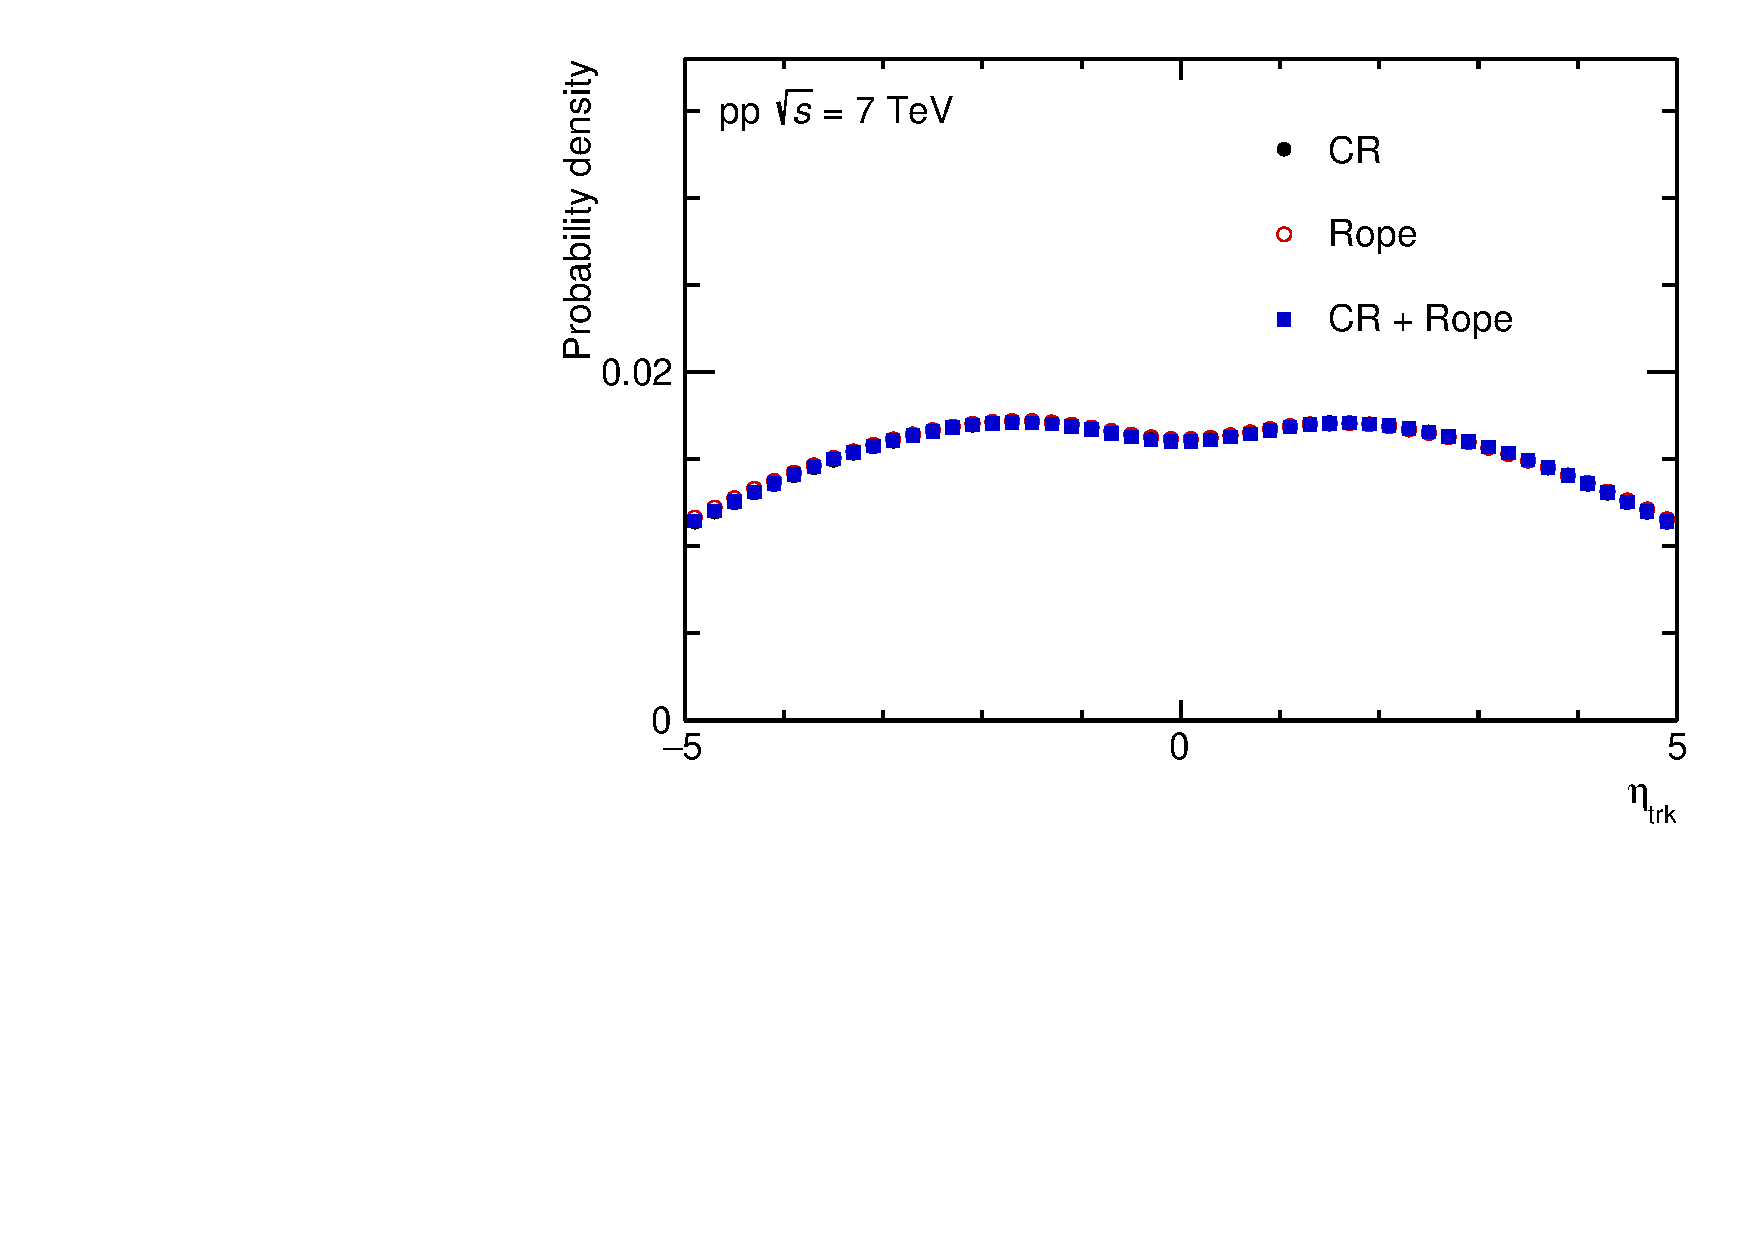
\includegraphics[width=.49\textwidth]{TrkEta}
		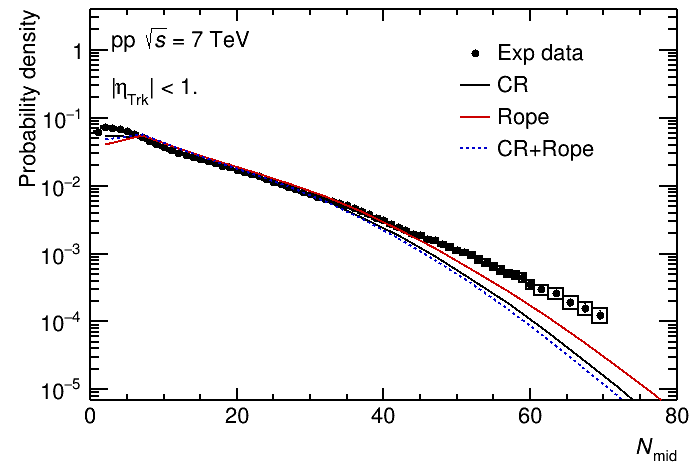
\includegraphics[width=.49\textwidth]{dNmiddEta}
	\end{center}
	\caption{Charged particle pseudo-rapidity ($\eta_\mathrm{trk}$)(left) and number of mid-rapidity tracks ($N_\mathrm{mid}$) (right) distribution for \pp collisions at \seven.  The experimental data are taken from~\cite{ALICE:2010mty}.}
	\label{fig:trkinfo}
\end{figure}

%1606.09456
Since rope and colour reconnection effects will rise with increasing event activity in \pp, it is desirable to use a discriminator for event activity which can both be measured in experiments and be sensible reproduced theoretically. Here we use the number of charged particles in the forward ($2 < |\eta| < 5$) direction.
%1806.11390
The average charged densities in each event for different string tension implementations are presented in Table~\ref{tab:eventclass}.

%1910.14397
The $\pT$-integrated yields of $\kzero$, $\kstar$, $\phi$, $\lmb$, $\Xi$ and $\Omega$ in \pp collisions at \seven with three configurations, are shown in Figure~\ref{fig:InclIntePar}. All of those three configurations can show an increase of all species as a function of multiplicity. The simulations are shown to compare well to the  data in Ref~\cite{ALICE:2016fzo, ALICE:2019etb}. The simulation results of  mesons, $\kzero$, $\kstar$, and $\phi$, show that the $\pT$-integrated yields are increasing faster for Rope mode than CR ones. In the contrary, the $\pT$-integrated yields of baryons, $\lmb$, $\Xi$, and $\Omega$, got by Rope are increasing slower than CR ones. The CR + Rope is the fastest in most cases, and can predict data the best. In addiction, only the CR + Rope can predict the multi-strange baryons ($\Xi$ and $\Omega$) well. These phenomena, above all, hint that the Rope mechanism will give larger production rates for strangeness in high multiplicity events, and the CR mode will give larger recombination rates for partons recombined to baryons.
%===================================================================
\begin{figure}[ht]
	\begin{center}
		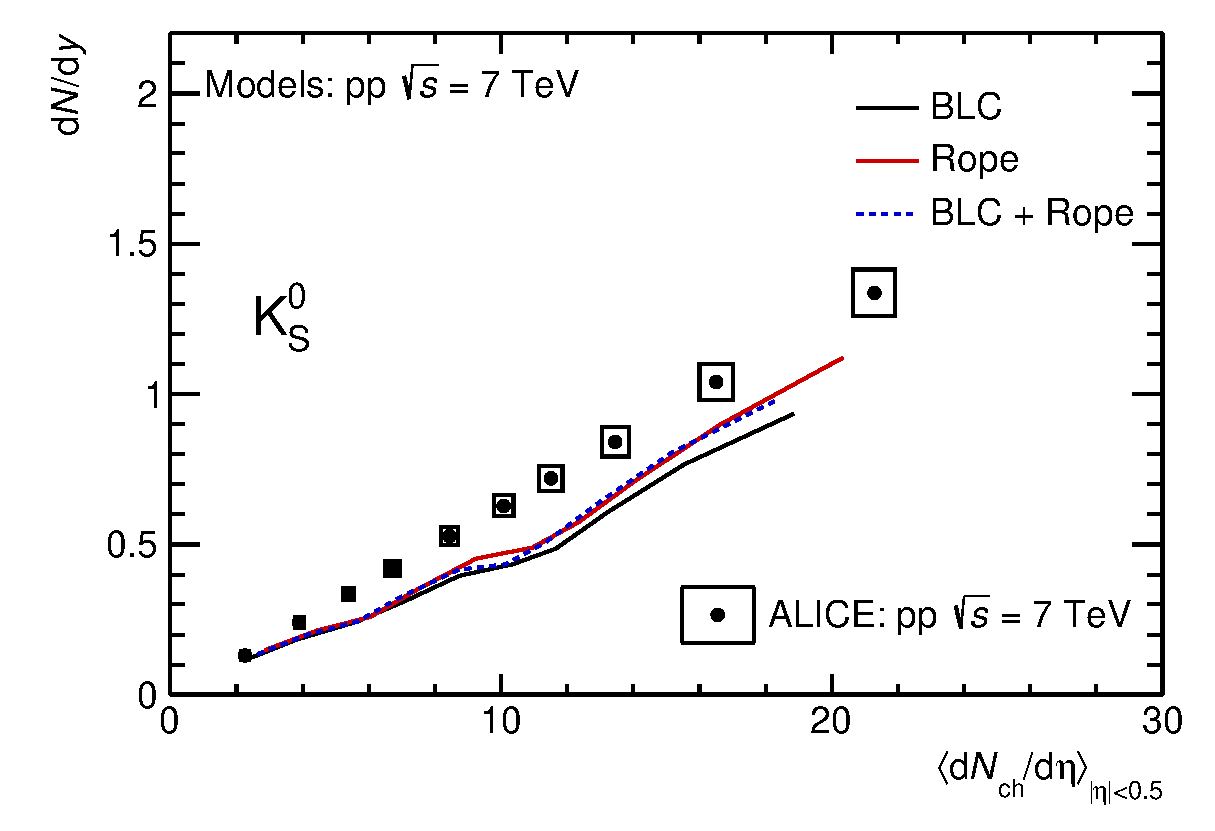
\includegraphics[width=.49\textwidth]{Kshort_InteSpectrum}
		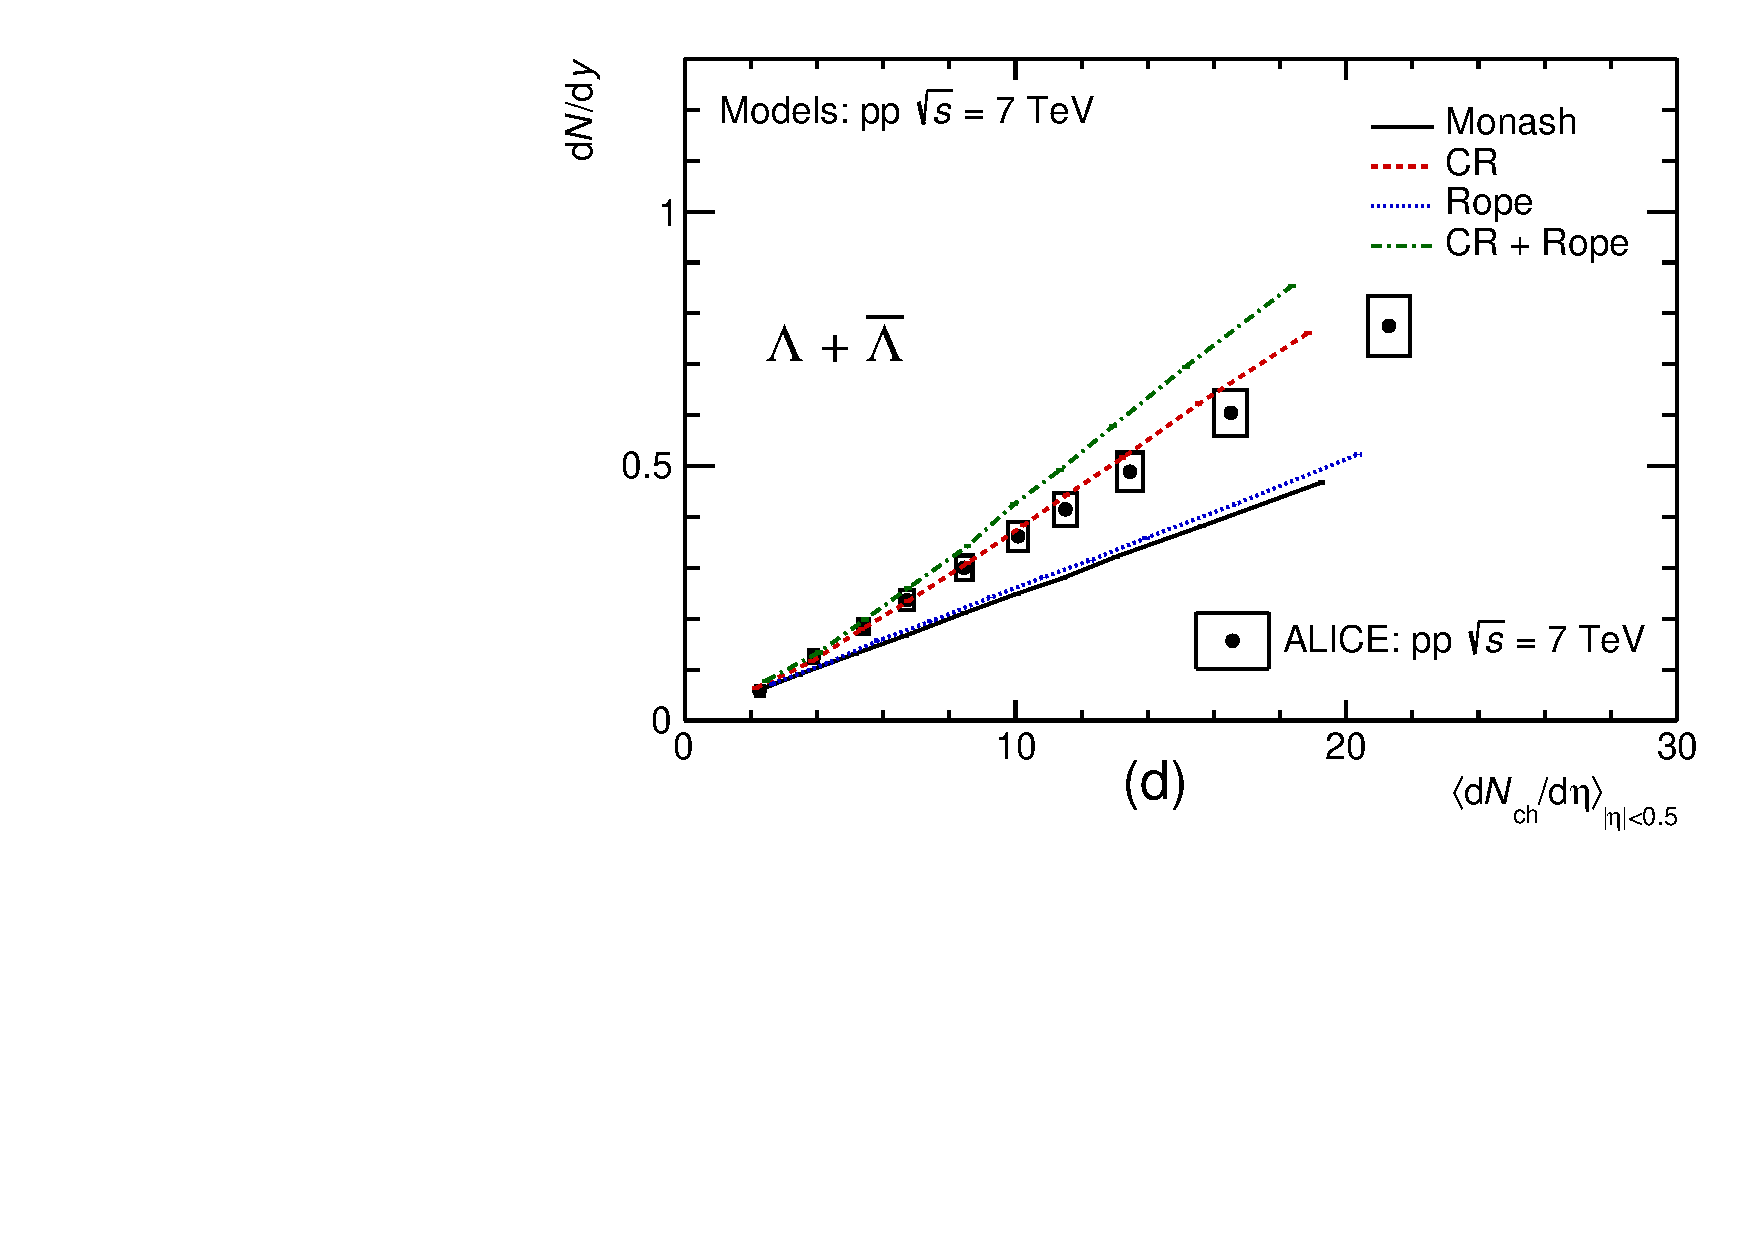
\includegraphics[width=.49\textwidth]{Lambda_InteSpectrum}
		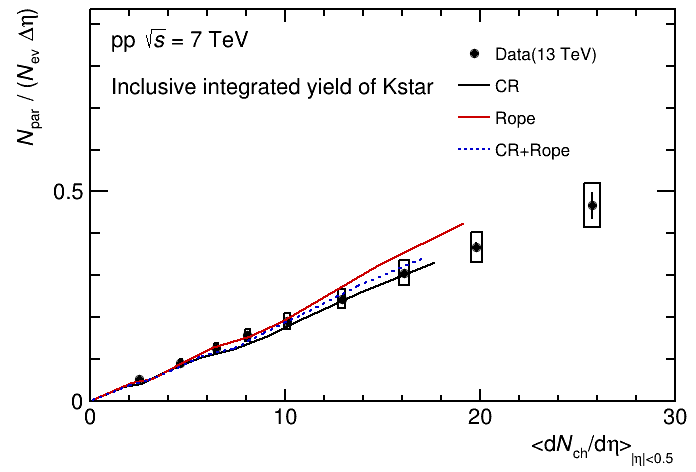
\includegraphics[width=.49\textwidth]{Kstar_InteSpectrum}
		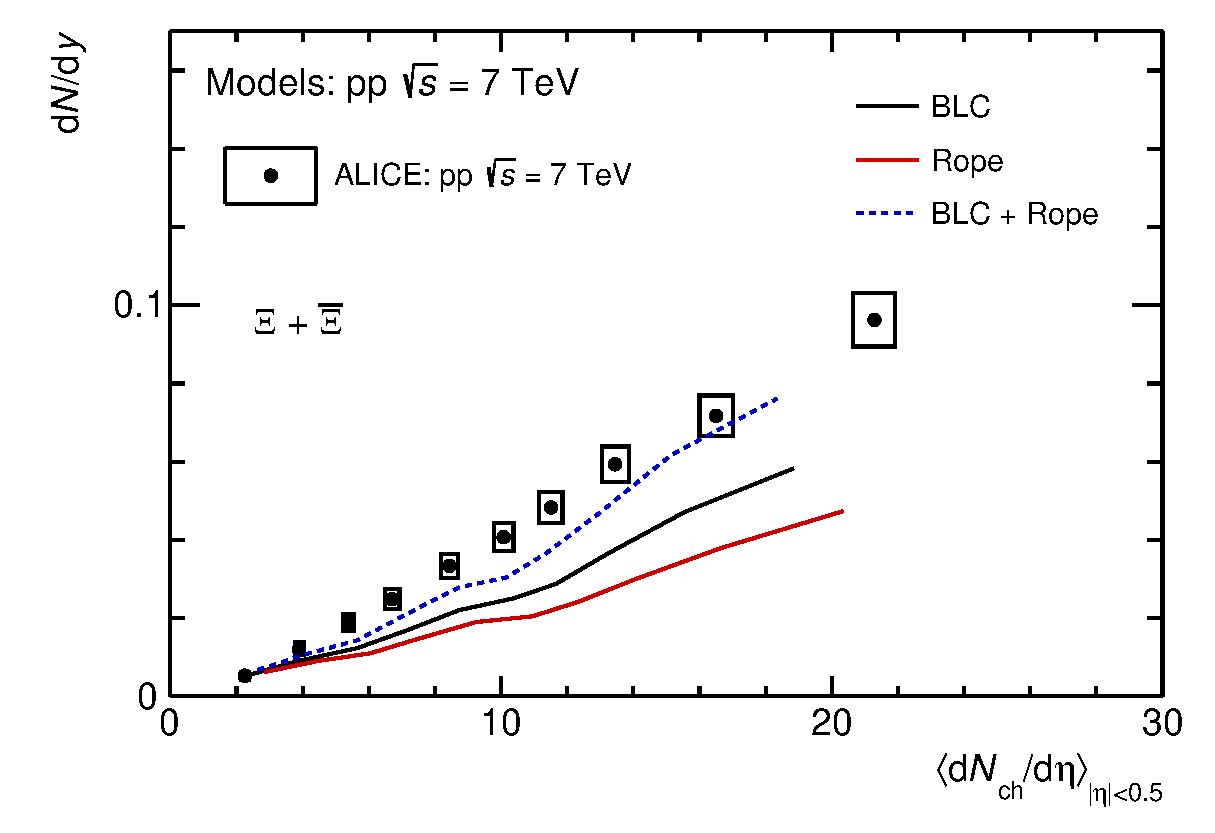
\includegraphics[width=.49\textwidth]{Xi_InteSpectrum}
		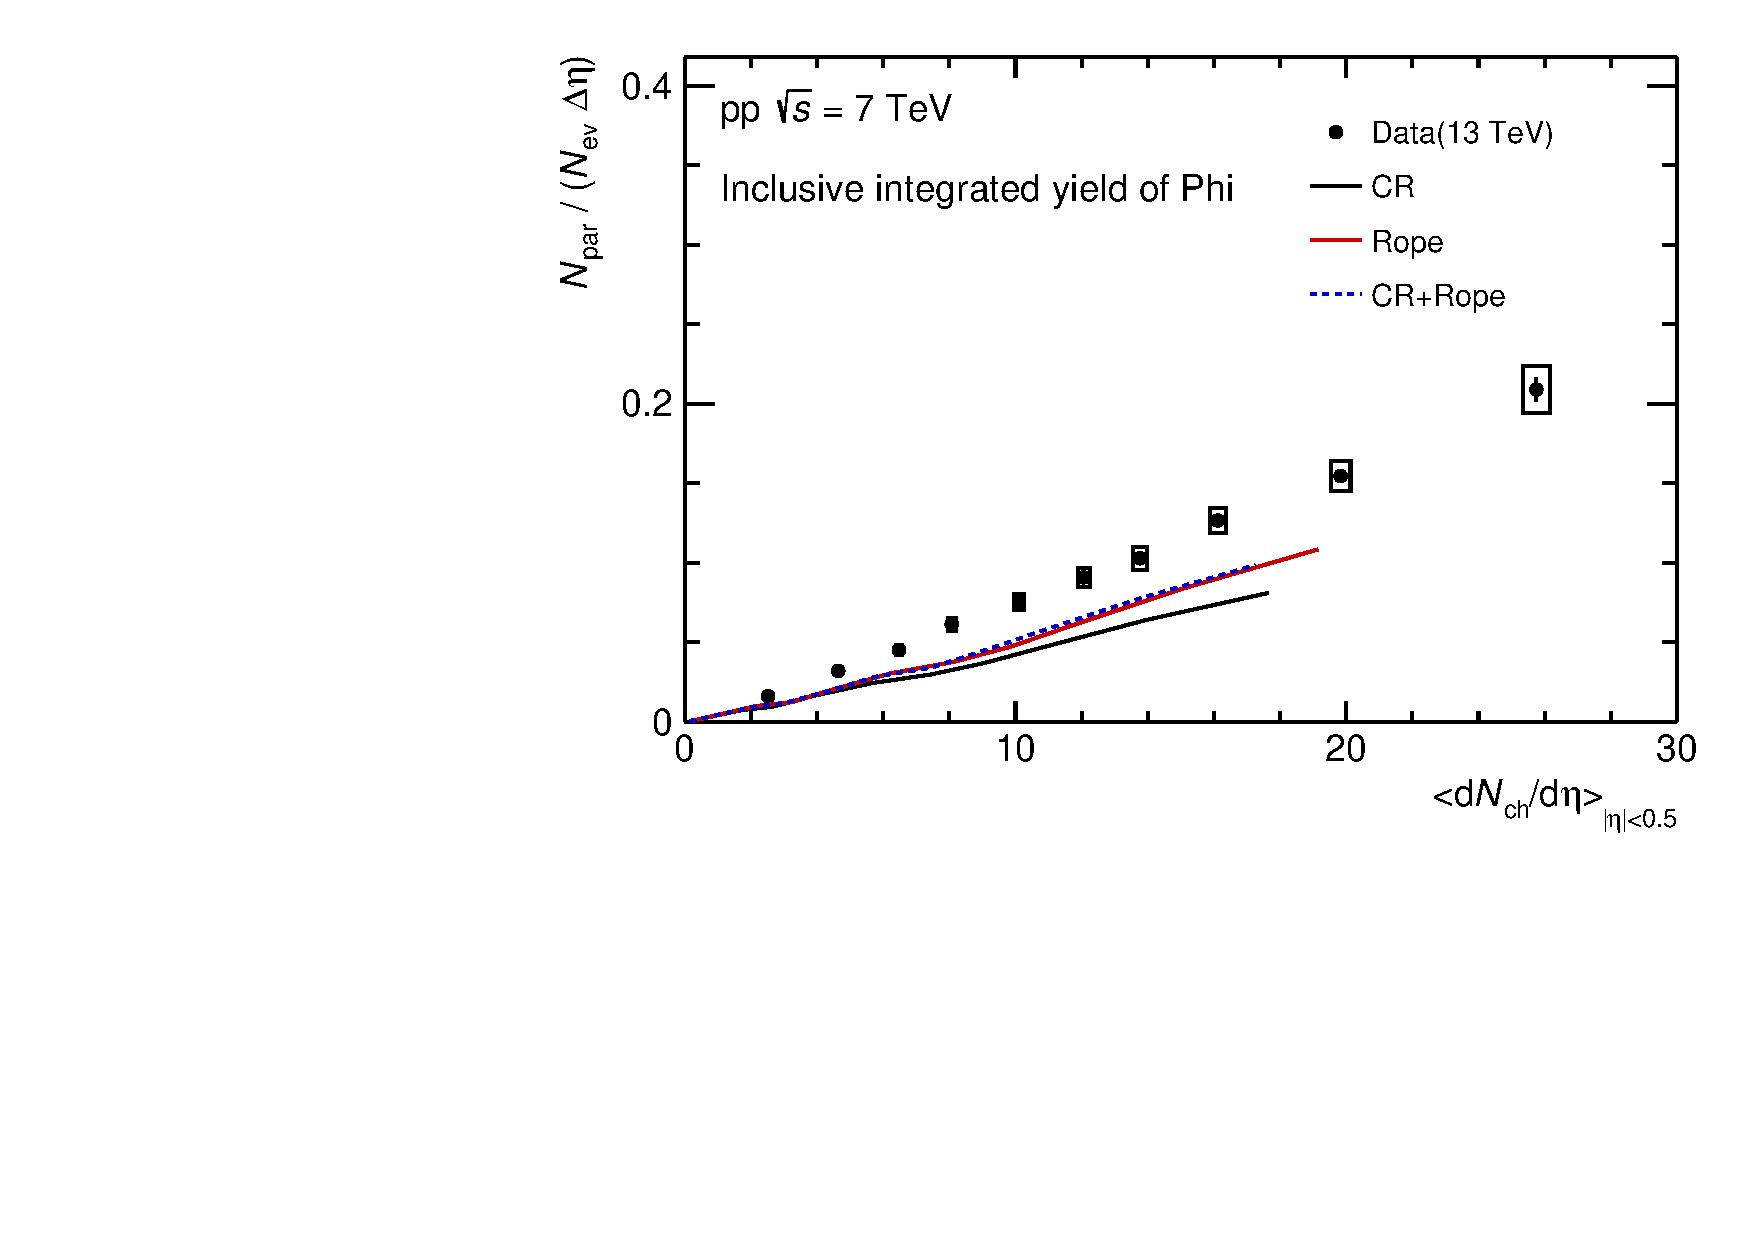
\includegraphics[width=.49\textwidth]{Phi_InteSpectrum}
		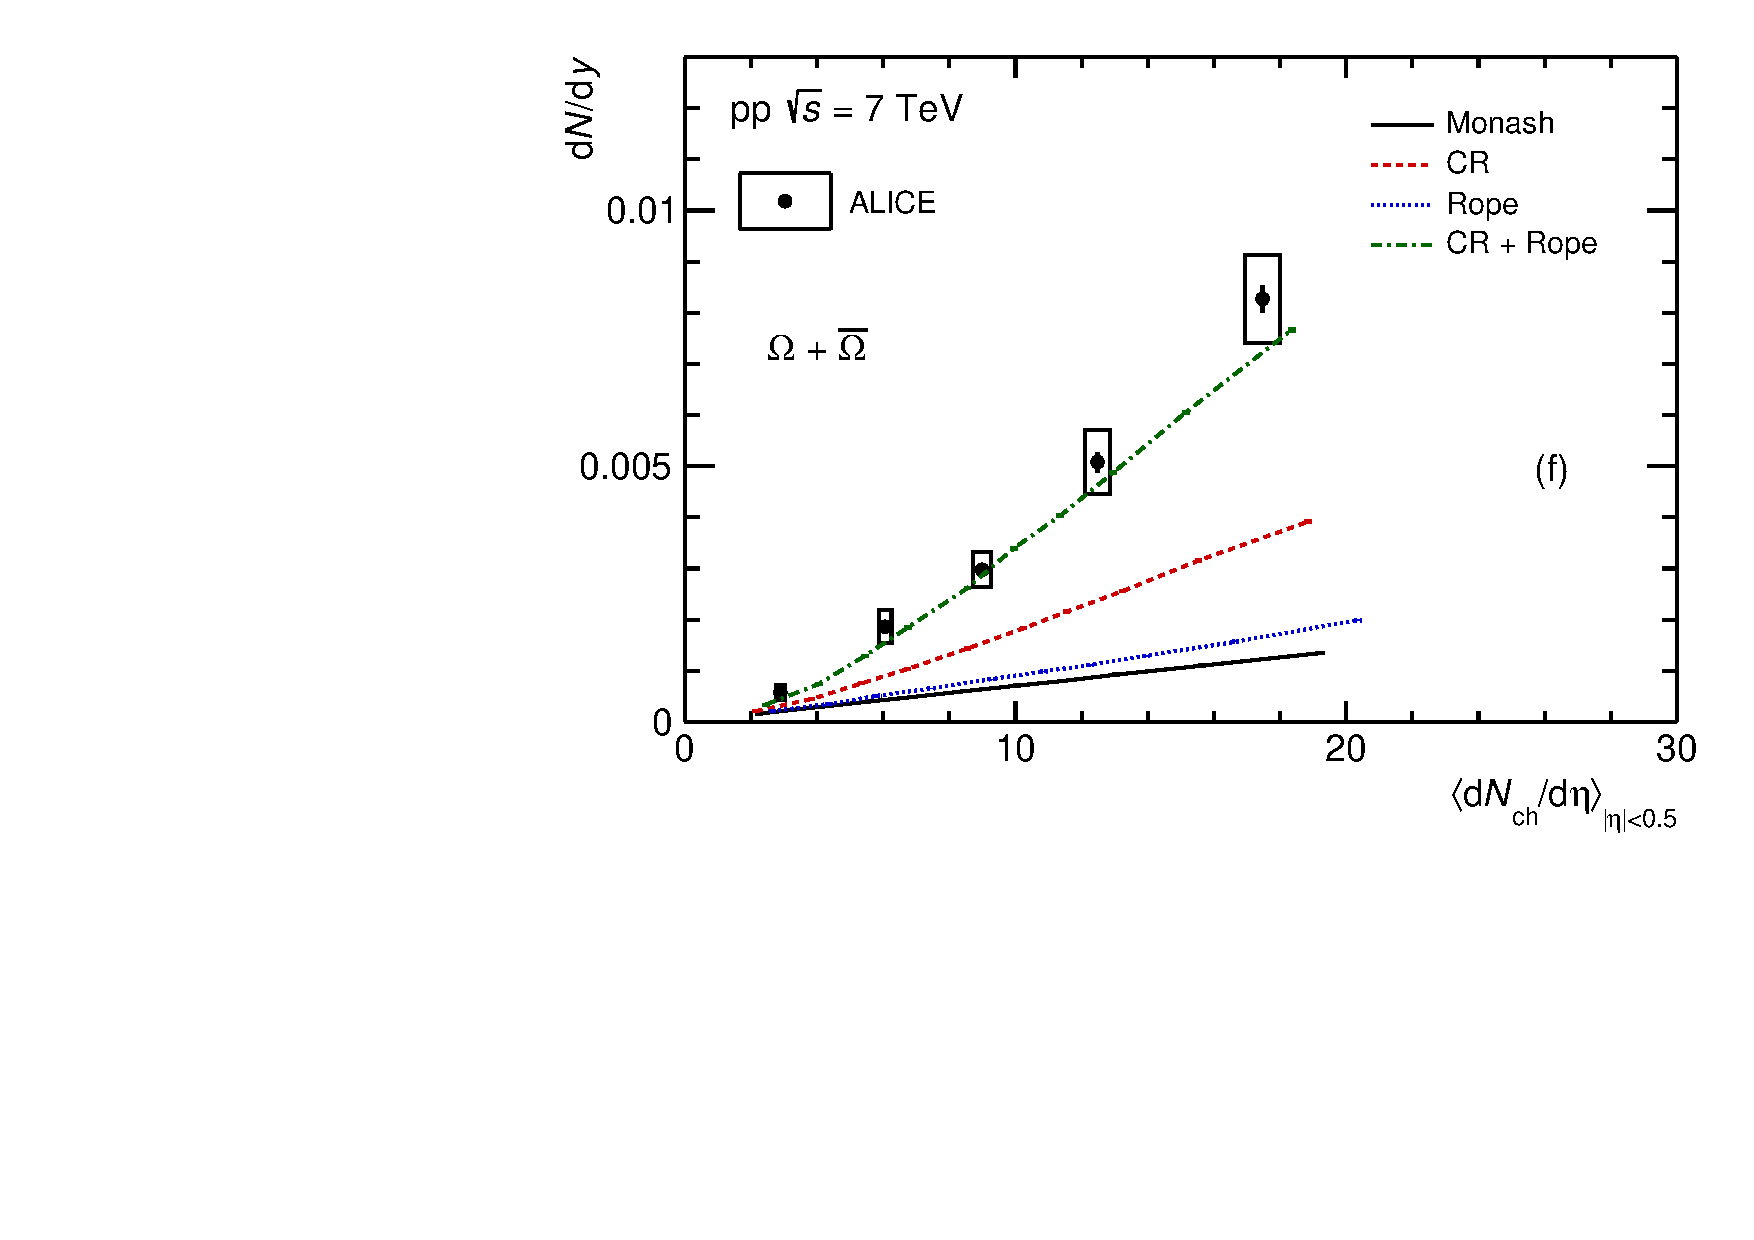
\includegraphics[width=.49\textwidth]{Omega_InteSpectrum}
	\end{center}
	\caption{$\pT$-integrated yields d$N/$d$y$ of various hadrons, $\kzero$, $\kstar$, $\phi$, $\lmb$, $\Xi$, and $\Omega$, as functions of $\langle\dndeta\rangle_{|\eta| < 0.5}$. The mesons yields are shown in the left plots, and the baryons yields are shown in the right plots. Model results are show for \pp collisions at \seven, data for \pp collisions at \seven and \thirteen (only for $\phi$ particle). The data point are taken from \cite{ALICE:2016fzo, ALICE:2019etb}.}
	\label{fig:InclIntePar}
\end{figure}

The corresponding hadrons to $\pi$ $\pT$-integrated ratios,  $\kzero/\pi$, $\phi/\pi$, $\Lambda/\pi$, $\Xi/\pi$, and $\Omega/\pi$ as functions of $\avdndeta_{|\eta| < 0.5}$ distributions in \pp collisions at \seven are studied in Figure~\ref{fig:InclIntePartoPiRatio}. 
%Due to the lack of experiment data reference for the $\kstar/\pi$ ratio, we only present the prediction results with the three models.
%All those models can quantitatively describe the experiment results well. 
The simulation results of mesons to $\pi$ ratio, $\kzero/\pi$, $\phi/\pi$ ,show that the models underestimate the experiment results, which also show the prediction of Rope mode is larger than the prediction of CR mode. In the contrary, the baryon to $\pi$ ratios, $\Lambda/\pi$, $\Xi/\pi$, and $\Omega/\pi$, got by Rope are less than CR ones. In addiction, only the CR + Rope gives the best prediction of the multi-strange baryons to $\pi$ ratios. %But this configuration overestimate the $\Lambda/\pi$ ratio and Rope describe the ratio well. For $\kzero/\pi$ and $\phi/\pi$ ratios, all the configuration slightly underestimate the data results.
\begin{figure}[ht]
	\begin{center}
		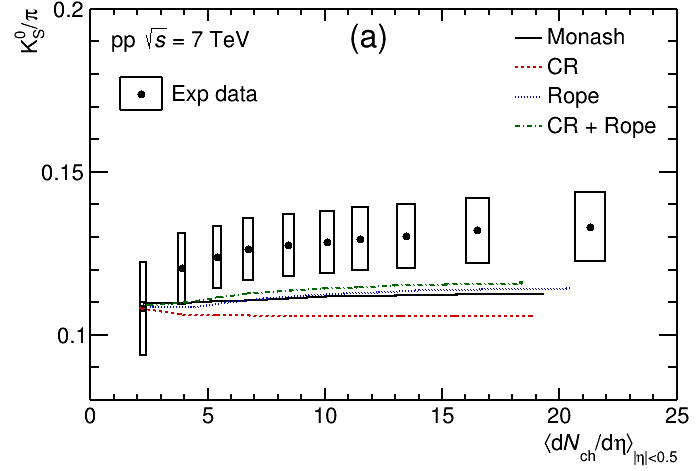
\includegraphics[width=.49\textwidth]{Kshort_PiRatio}
		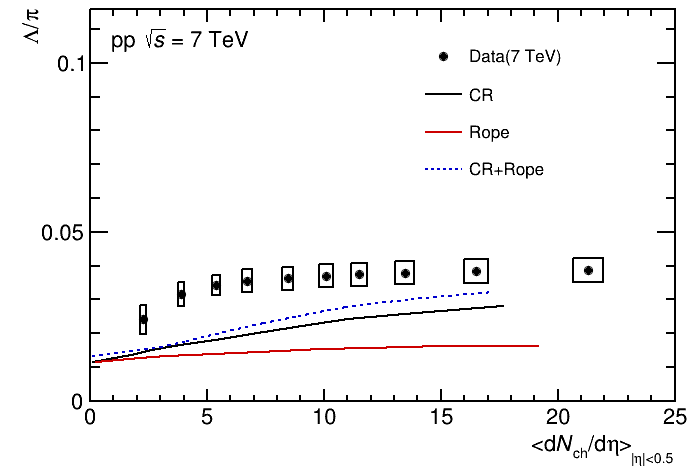
\includegraphics[width=.49\textwidth]{Lambda_PiRatio}
		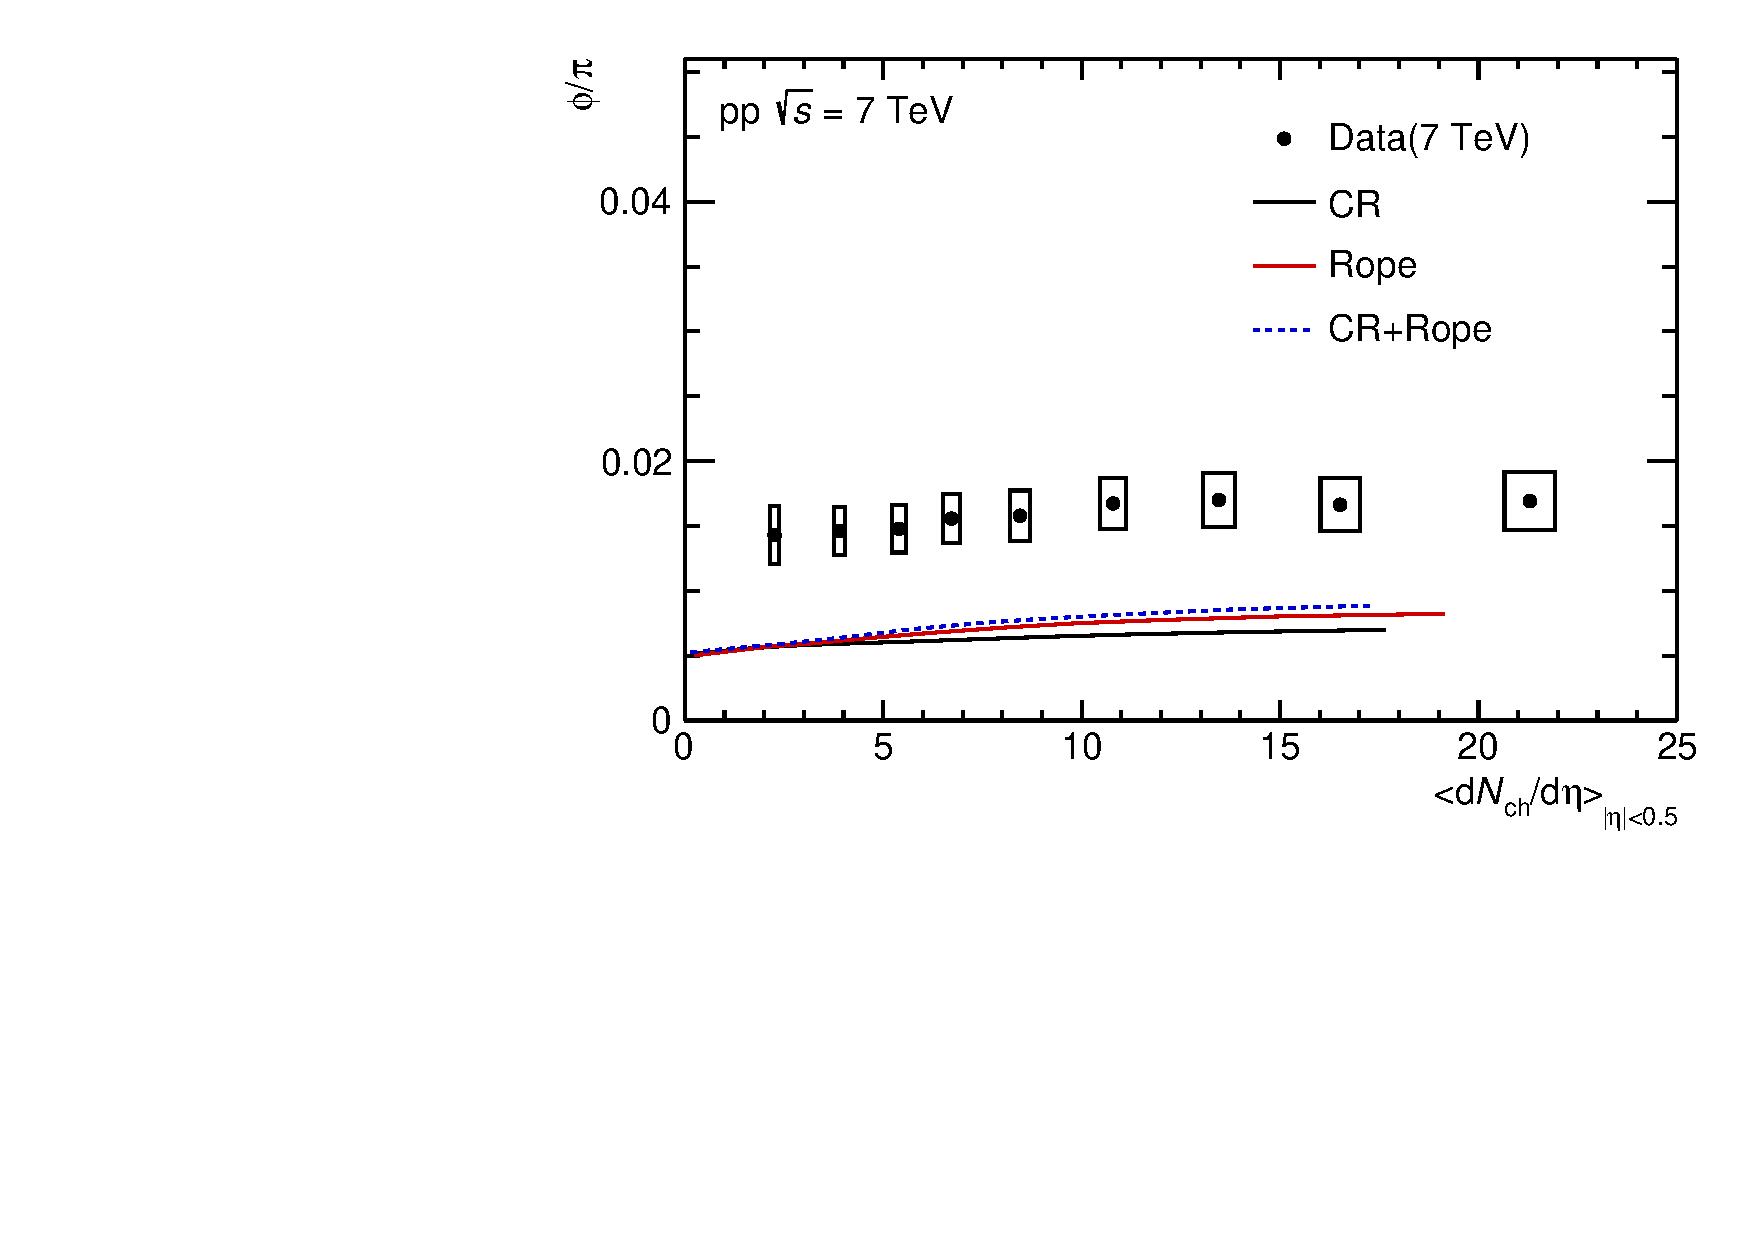
\includegraphics[width=.49\textwidth]{Phi_PiRatio}	
		%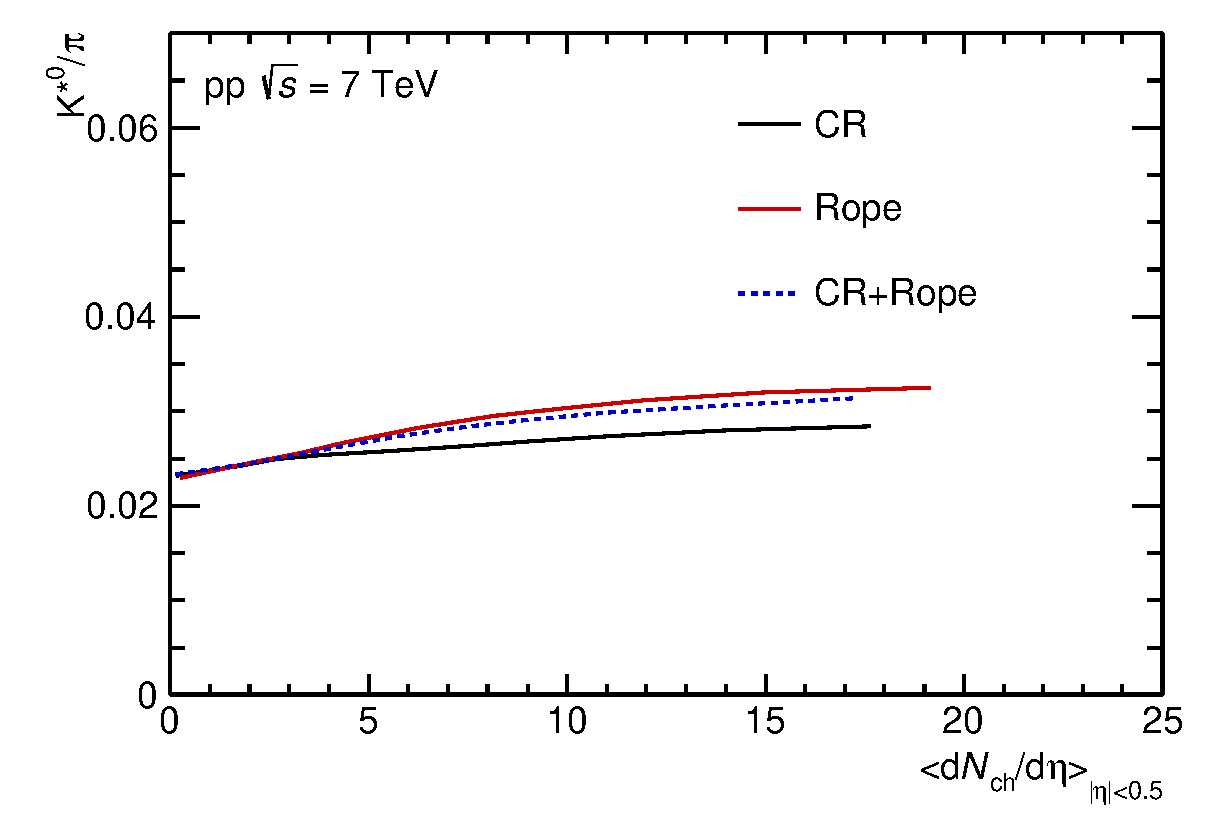
\includegraphics[width=.49\textwidth]{Kstar_PiRatio}
		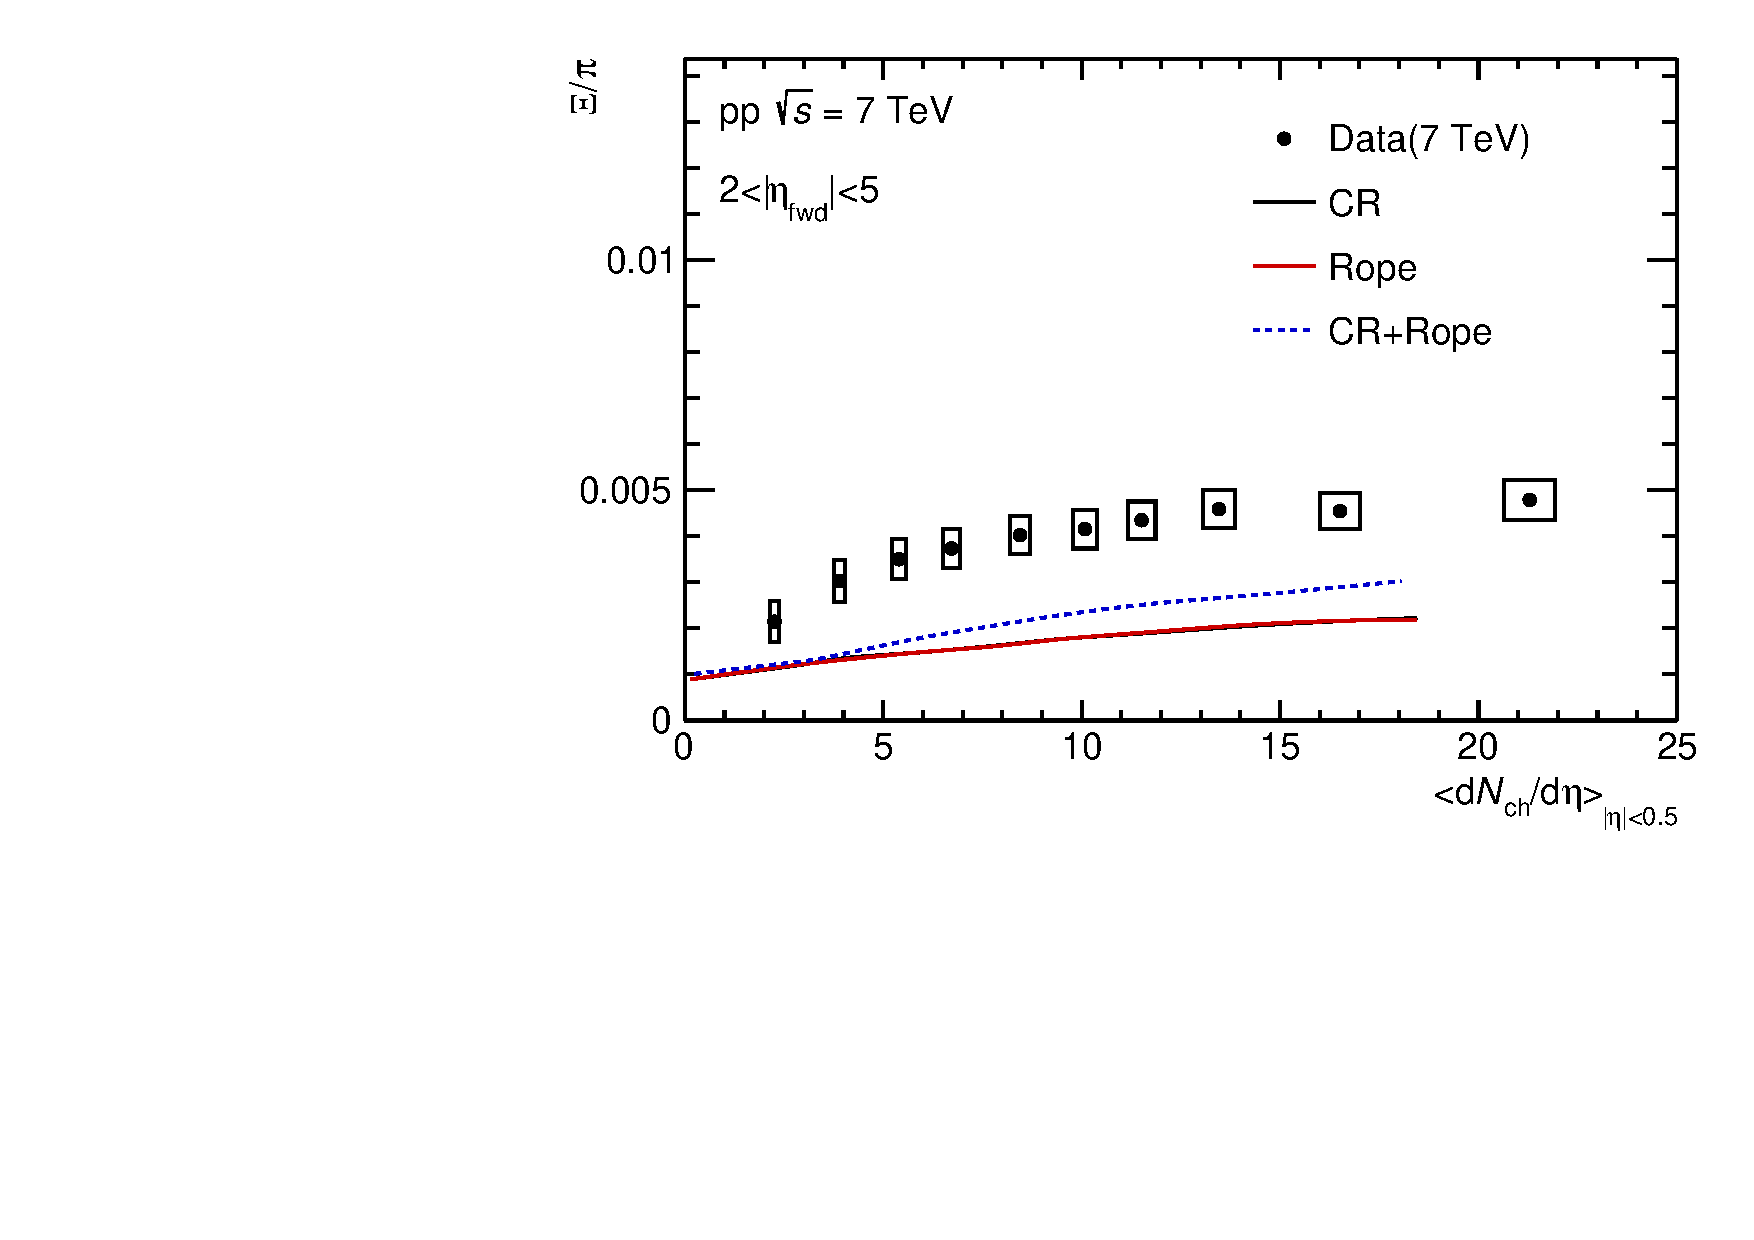
\includegraphics[width=.49\textwidth]{Xi_PiRatio}
		\begin{minipage}{0.49\textwidth}
			$\space$
		\end{minipage}
		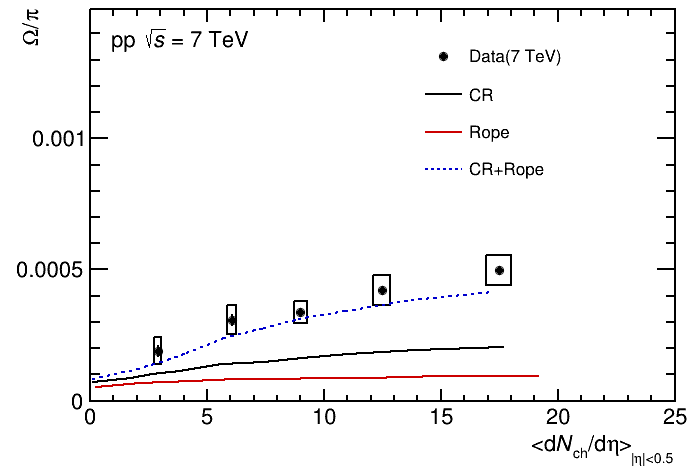
\includegraphics[width=.49\textwidth]{Omega_PiRatio}
	\end{center}
	\caption{Hadrons to $\pi$ $\pT$-integrated ratios, $\kzero/\pi$, $\phi/\pi$, $\Lambda/\pi$, $\Xi/\pi$, and $\Omega/\pi$, as function of $\langle\dndeta\rangle_{|\eta| < 0.5}$ distributions in \pp collisions at \seven.  The mesons to $\pi$ ratios are shown in the left plots, and the baryons to $\pi$ ratios are shown is the right plots. The data point are taken from  \cite{ALICE:2016fzo, ALICE:2018pal}.}
	\label{fig:InclIntePartoPiRatio}
\end{figure}


%===================================================================
The $\pT$-differential spectra of hadrons at midrapidity ($|y| < 0.5$) in minimum bias \pp collisions at \seven are presented in Figure~\ref{fig:InclParSpect}. All those models can predict the experimental data. Prediction results are almost no different among those three configurations. Only for $\Omega~(sss)$ particle, the CR + Rope can simulate well.
\begin{figure}[ht]
	\begin{center}
		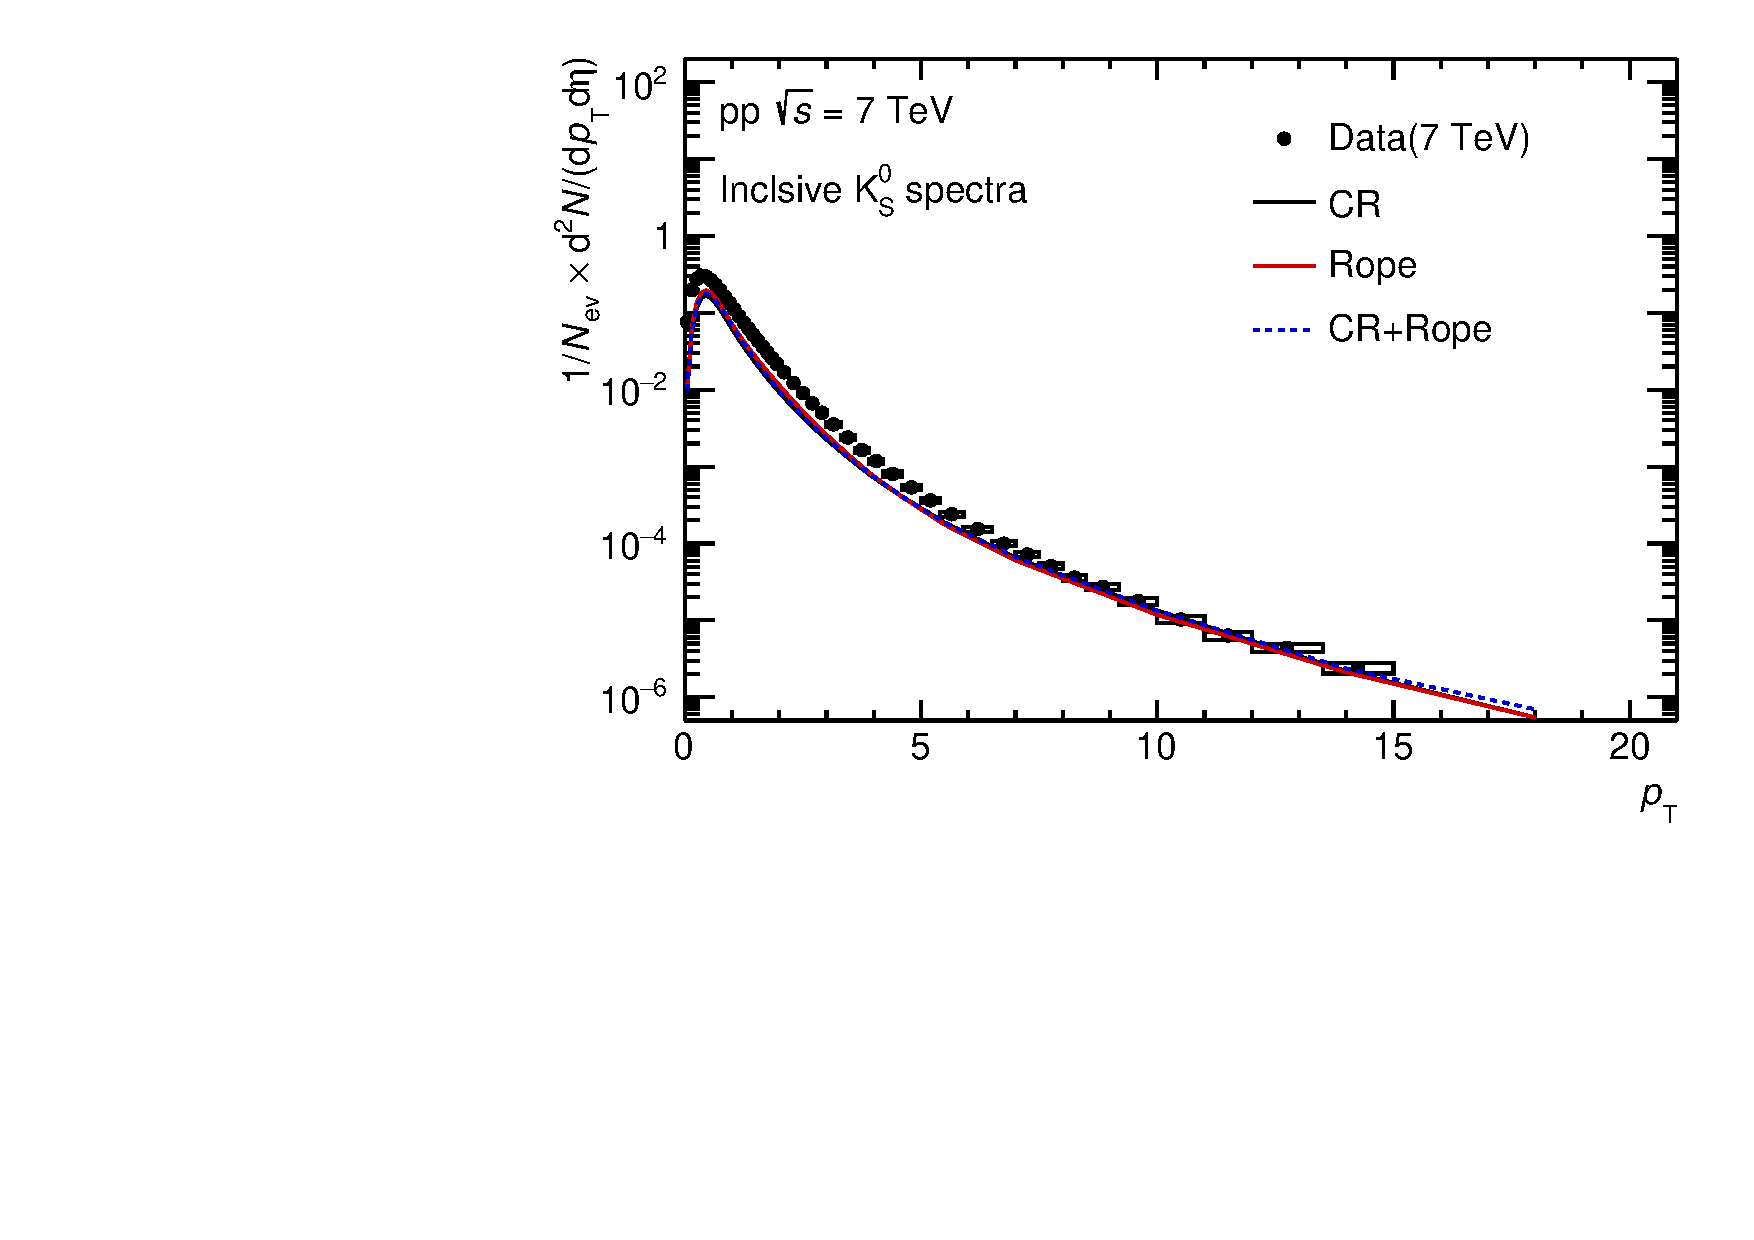
\includegraphics[width=.48\textwidth]{Incl_KshortSpect}
		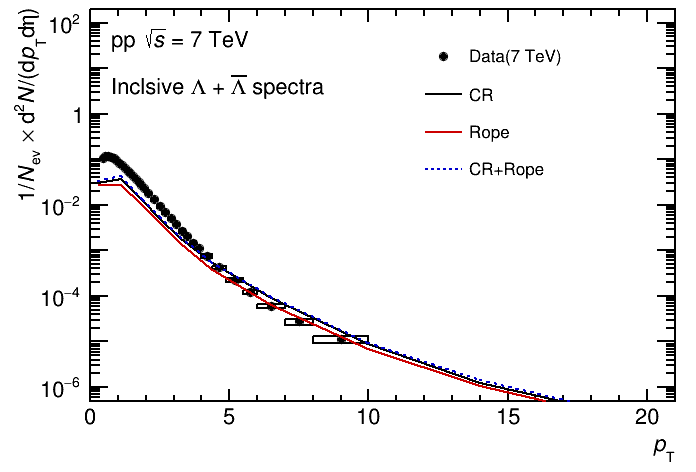
\includegraphics[width=.48\textwidth]{Incl_LambdaSpect}
		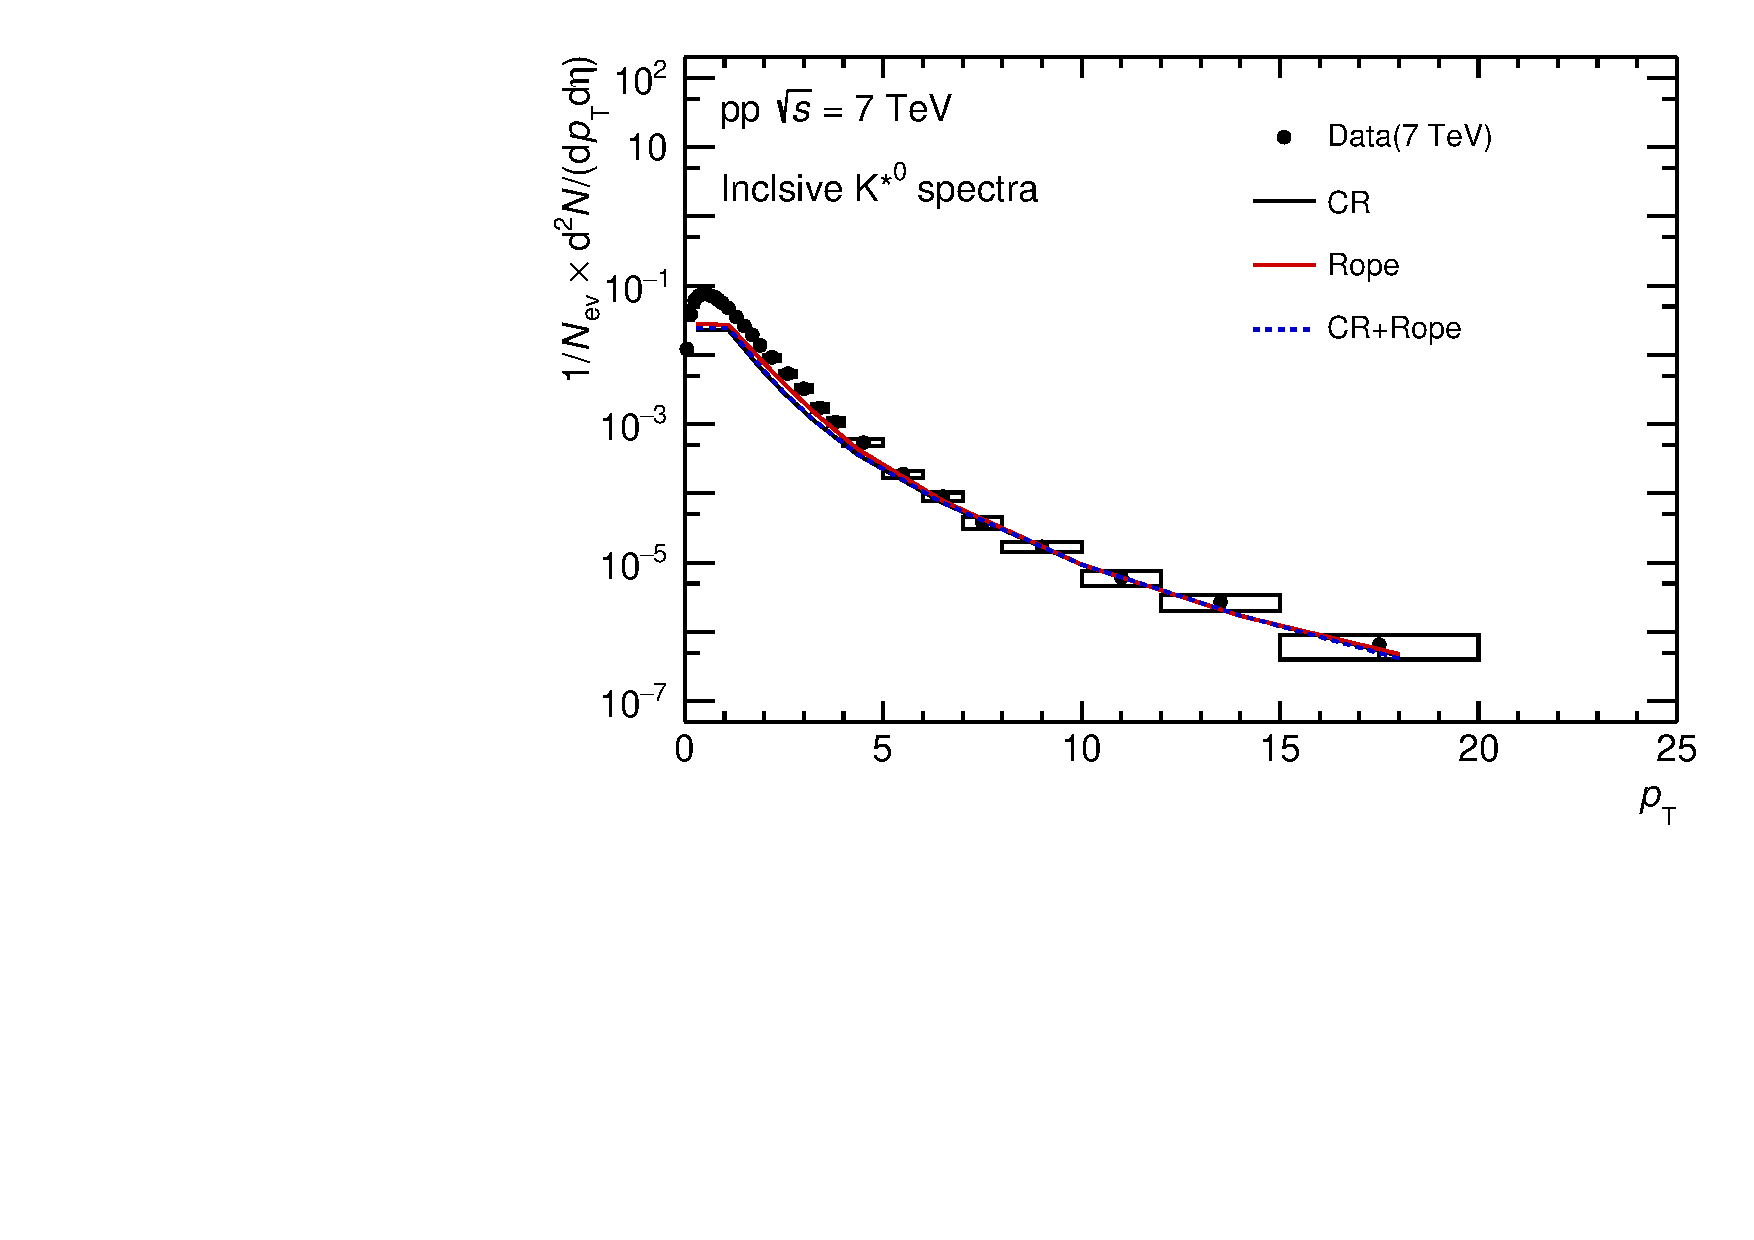
\includegraphics[width=.48\textwidth]{Incl_KstarSpect}
		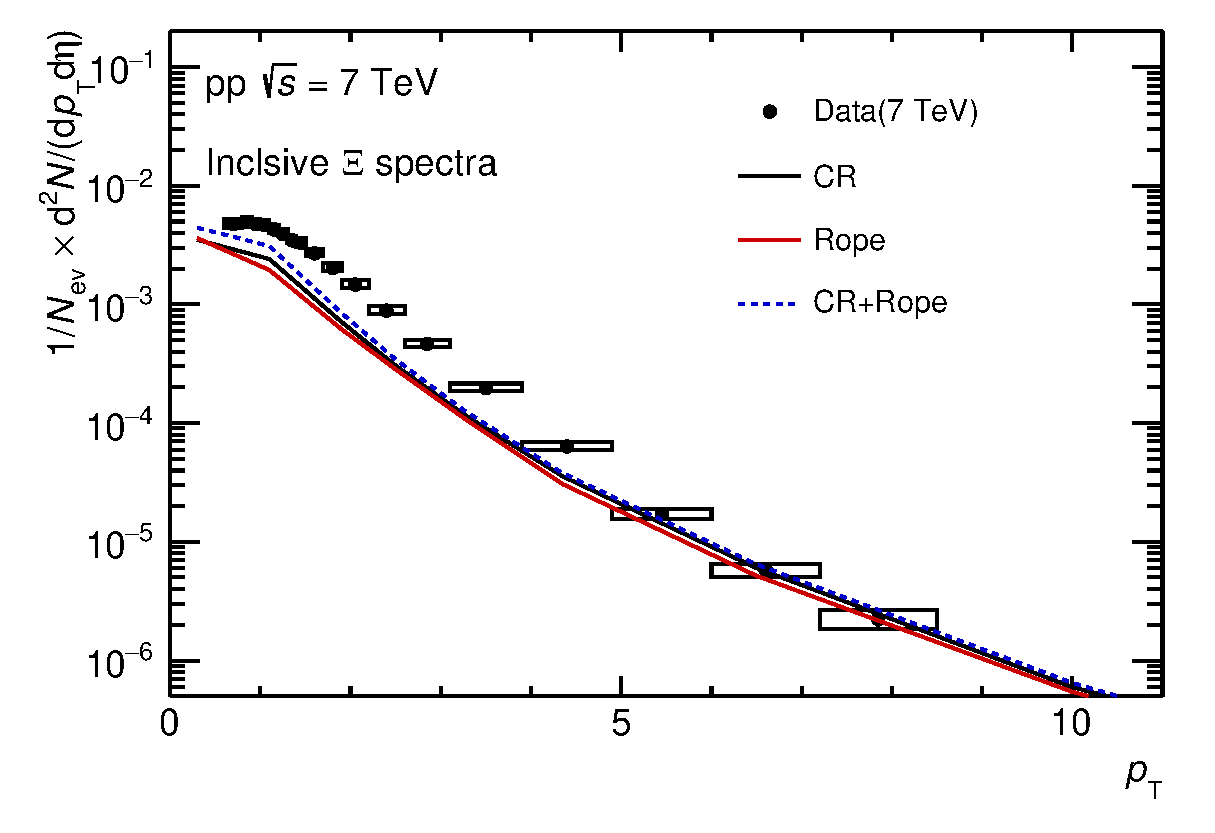
\includegraphics[width=.48\textwidth]{Incl_XiSpect}
		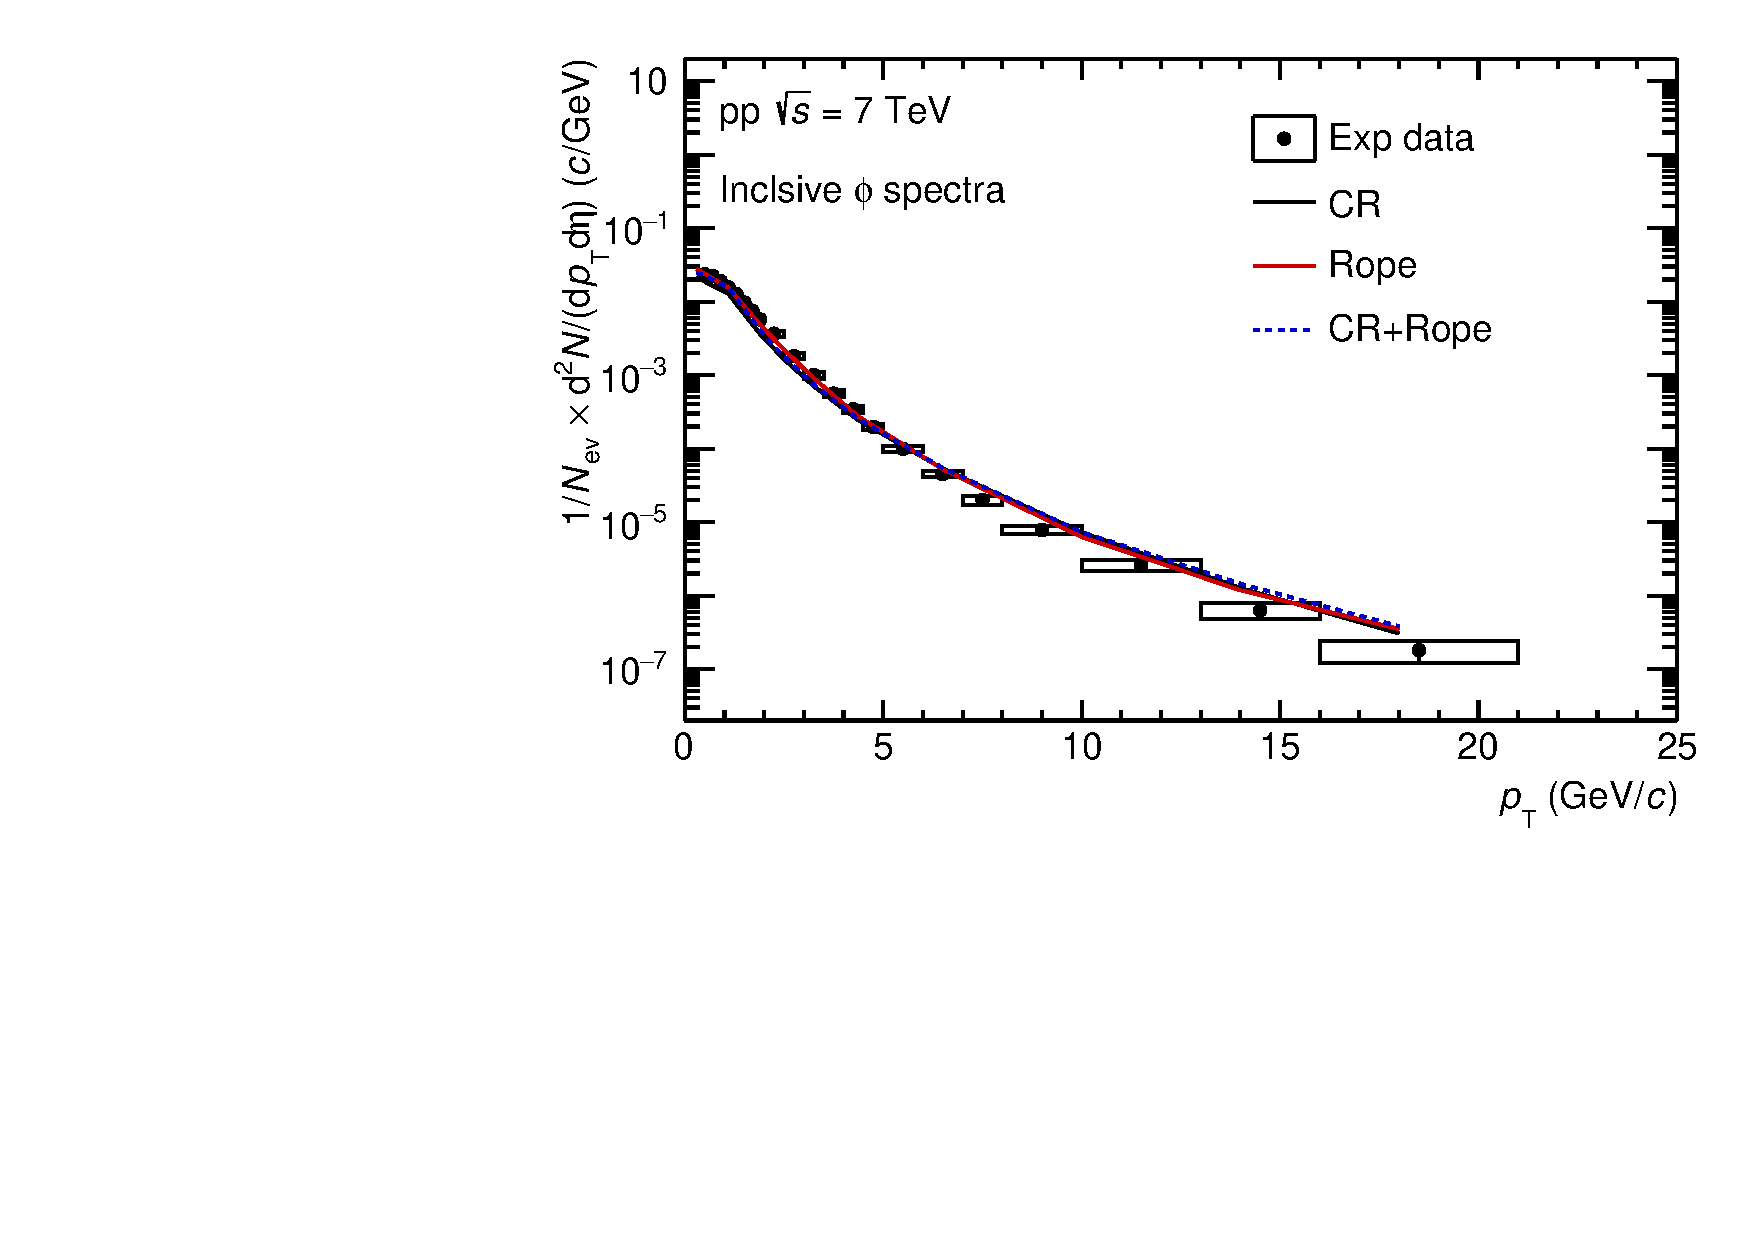
\includegraphics[width=.48\textwidth]{Incl_PhiSpect}
		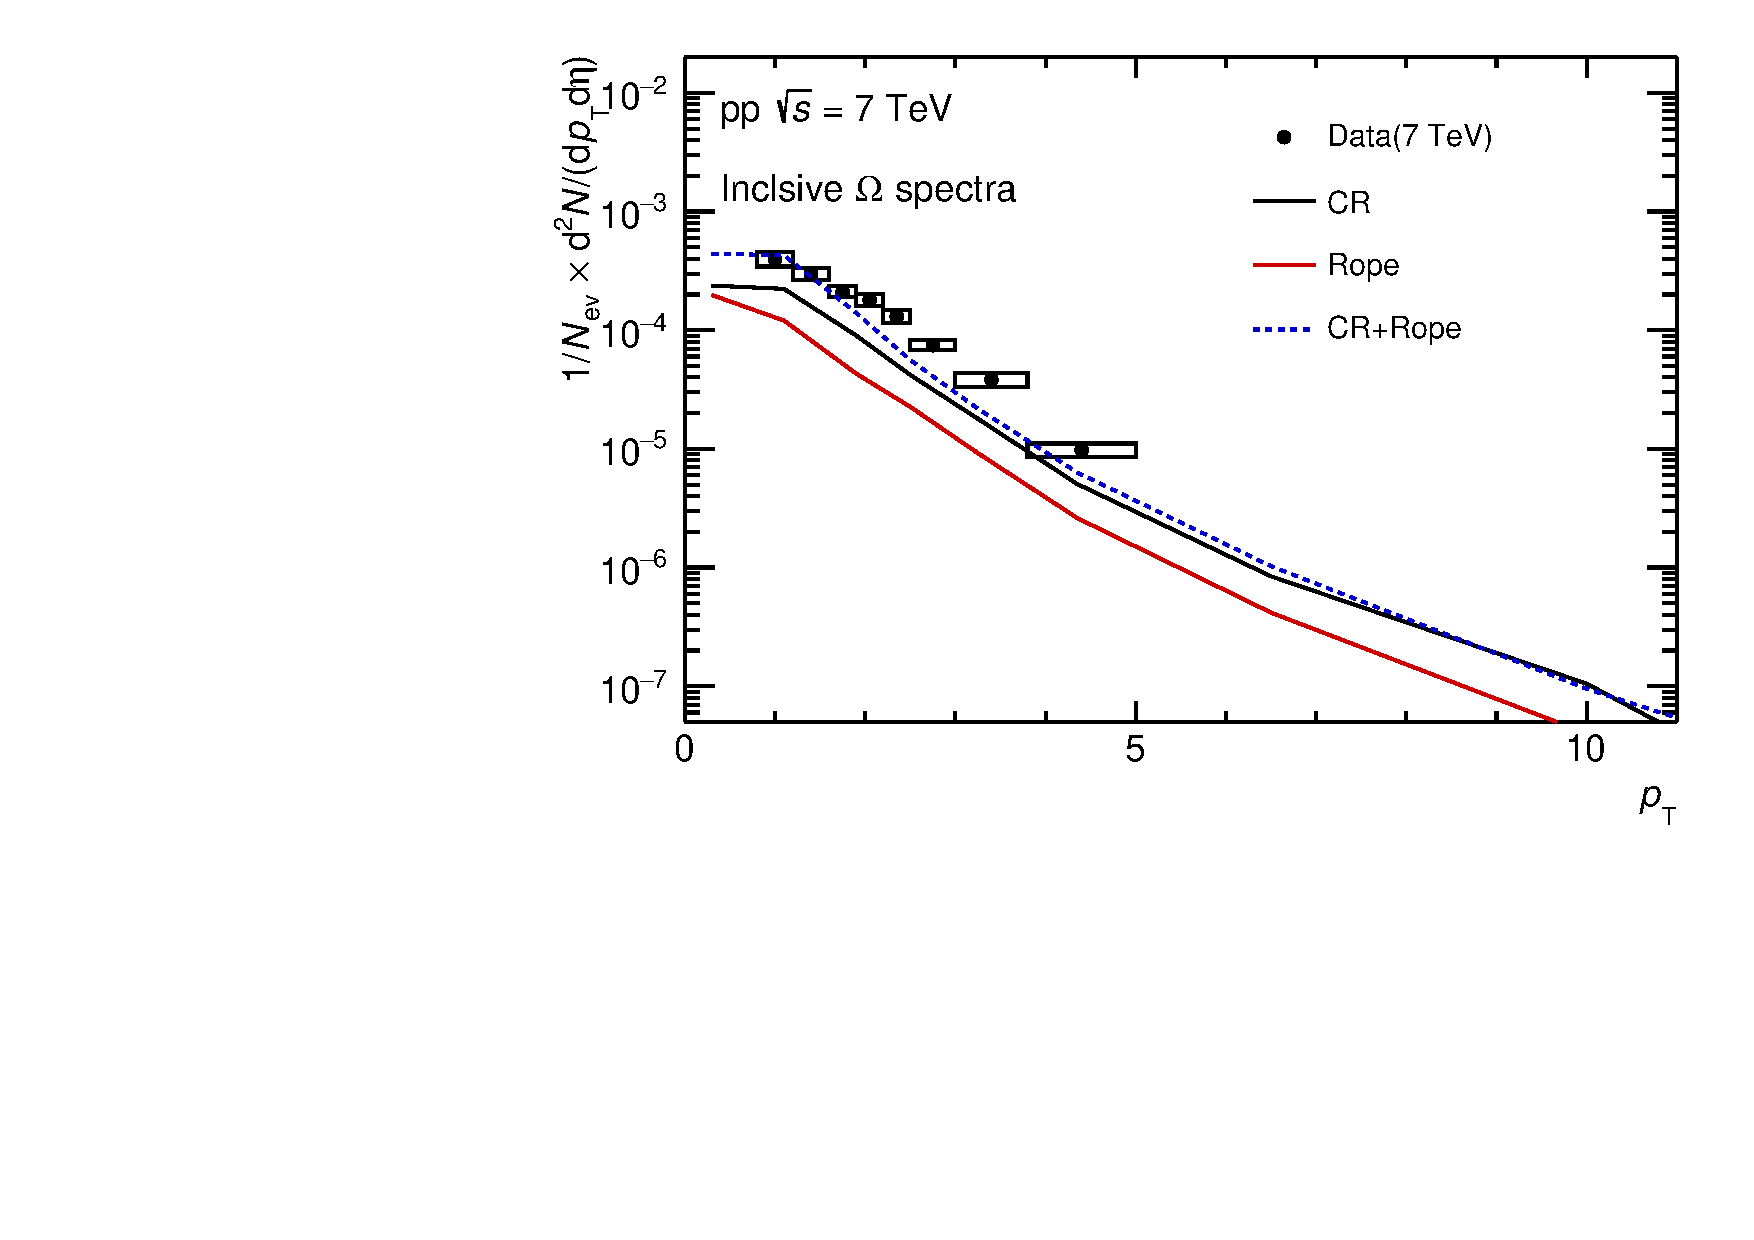
\includegraphics[width=.48\textwidth]{Incl_OmegaSpect}
	\end{center}
	\caption{Transverse momentum spectra of strange hadrons measured at midrapidity $|y| < 0.5$ in minimum bias \pp collisions at \seven TeV. Data taken from \cite{ALICE:2020jsh, Basak:2012jy, ALICE:2019hyb}.}
	\label{fig:InclParSpect}
\end{figure}

%===================================================================
%Transverse momentum dependence of $\Lambda/\kzero$, $\phi/\kzero$ and $\kstar/\kzero$ yields ratios in \pp collisions at \seven for high (II) and low (X) multiplicity classes are shown in Figure~\ref{fig:InclParRatioCentPeri}. The $\Lambda/\kzero$ ratio enhancement at intermediate $\pT$ for high multiplicity \pp collisions are shown in those there models. But the CR and CR + Rope model overestimate the enhancement, and the Rope model underestimate it. The $\phi/\kzero$ and $\kstar/\kzero$ yields ratios increase at low $\pT$ and saturate for $\pT \gtrsim 2.5$~\GeVc. The three models can describe this trend well. 
%\begin{figure}[ht]
%	\begin{center}
%		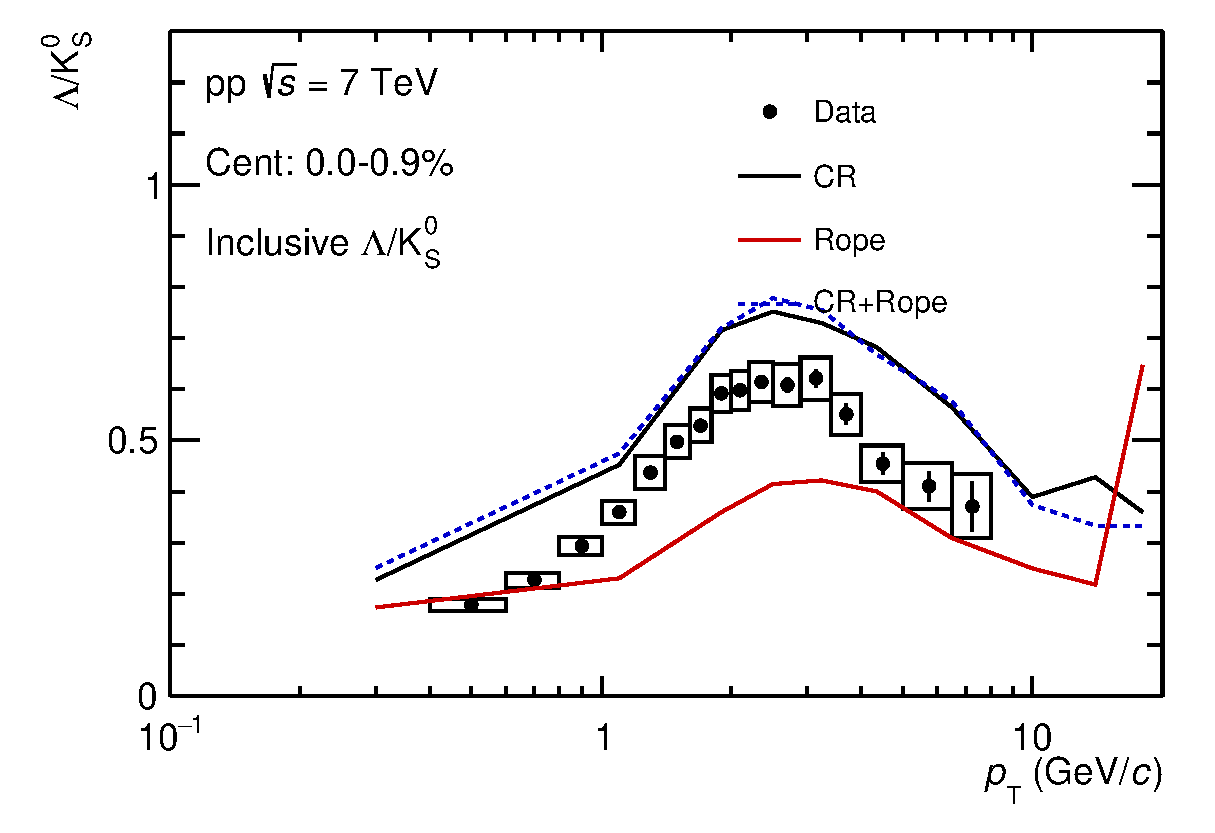
\includegraphics[width=.48\textwidth]{LKRatio_Incl_Center}
%		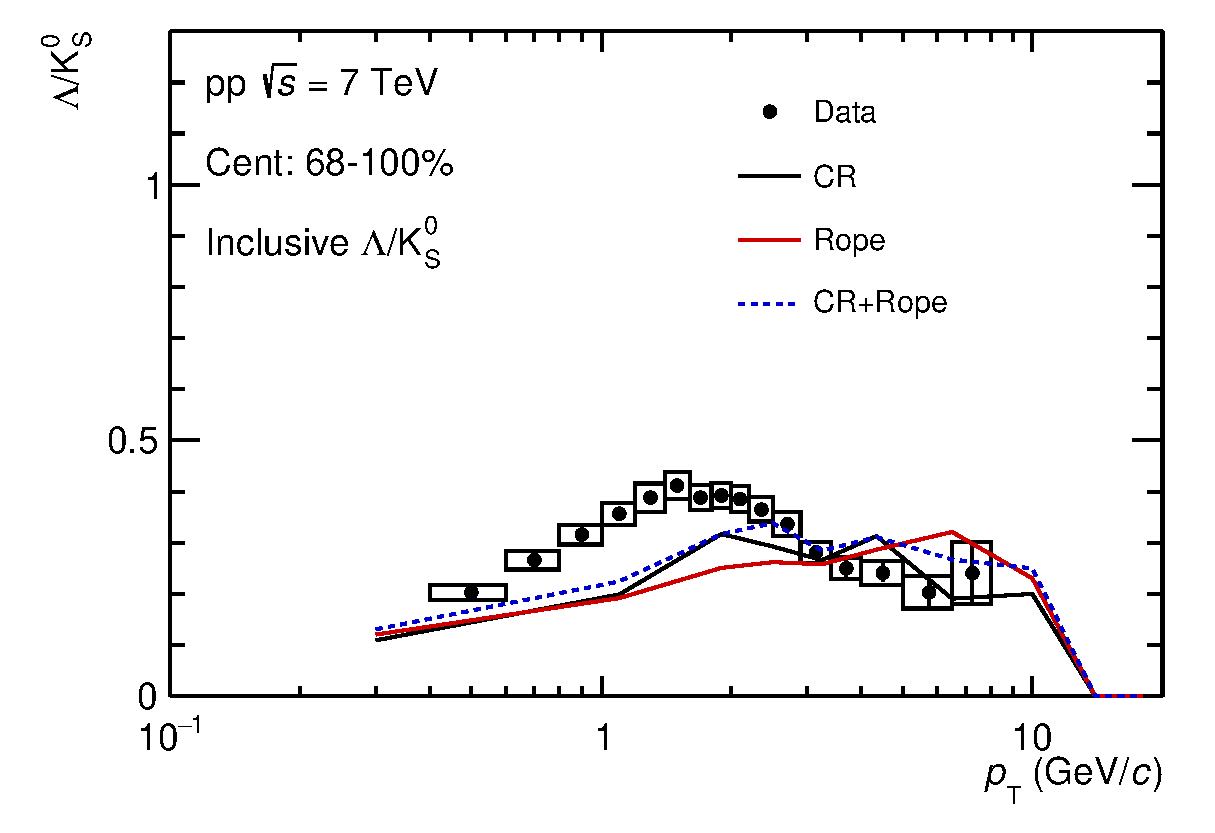
\includegraphics[width=.48\textwidth]{LKRatio_Incl_Peripheral}
%		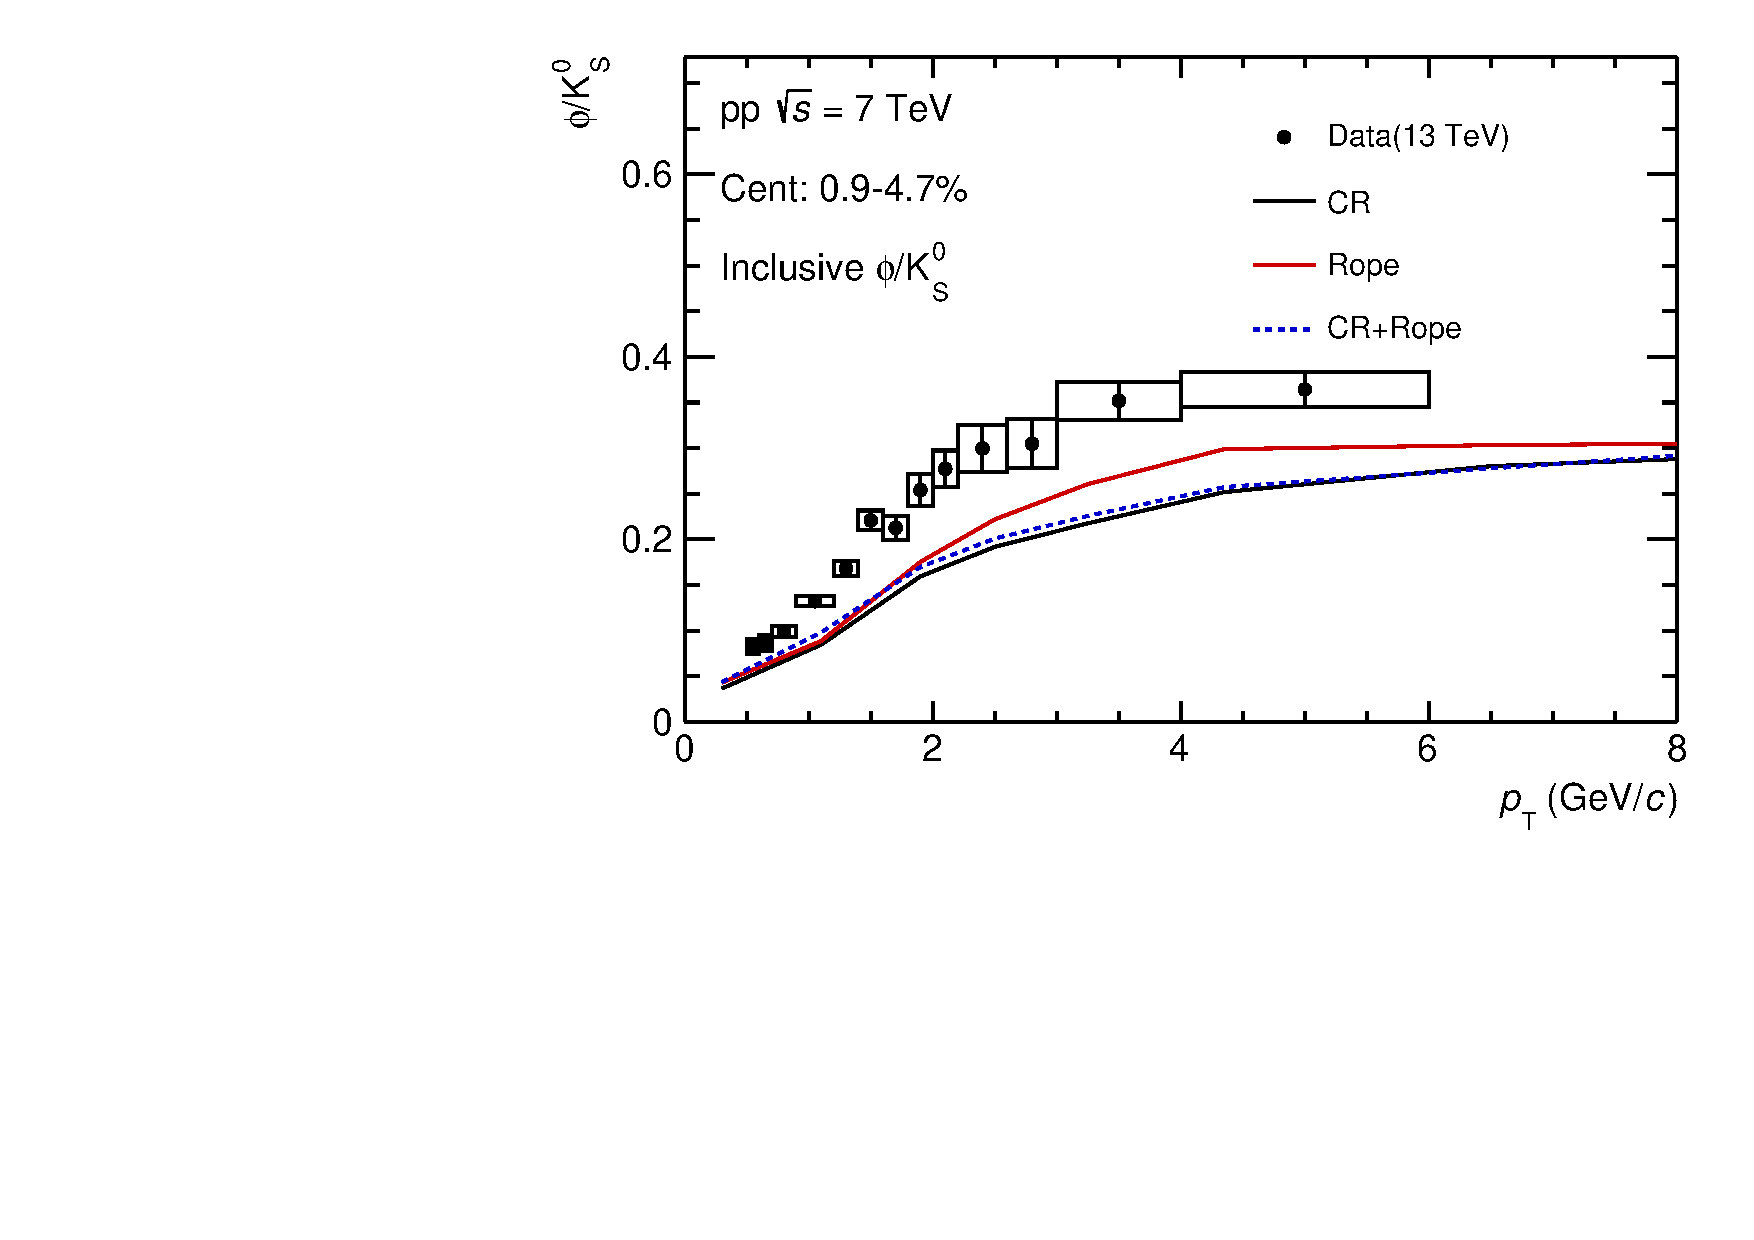
\includegraphics[width=.48\textwidth]{PhiKRatio_Incl_Center}
%		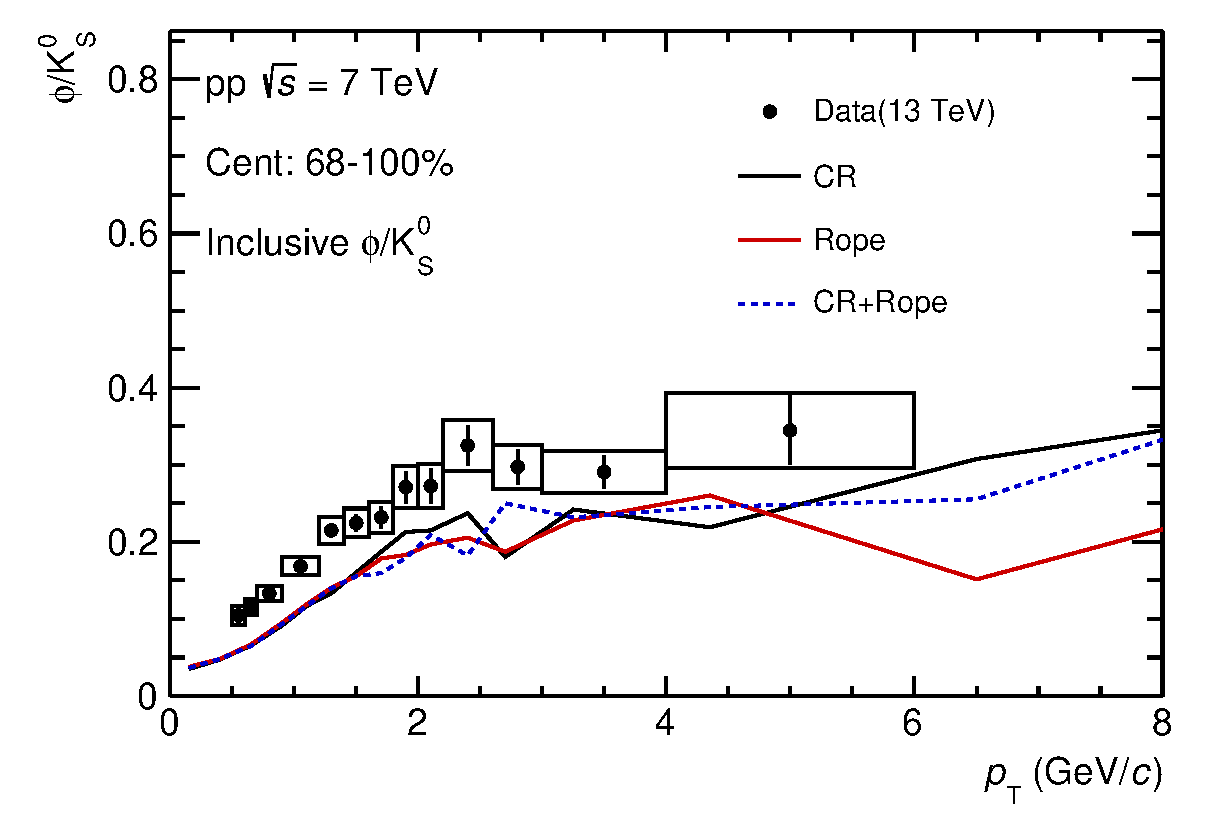
\includegraphics[width=.48\textwidth]{PhiKRatio_Incl_Peripheral}
%		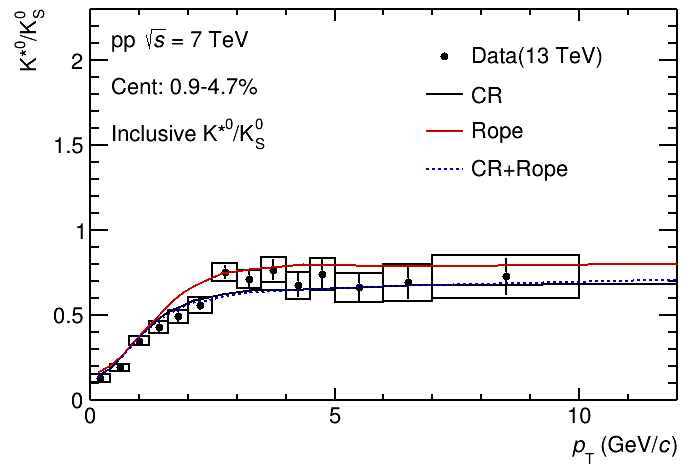
\includegraphics[width=.48\textwidth]{KstarKRatio_Incl_Center}
%		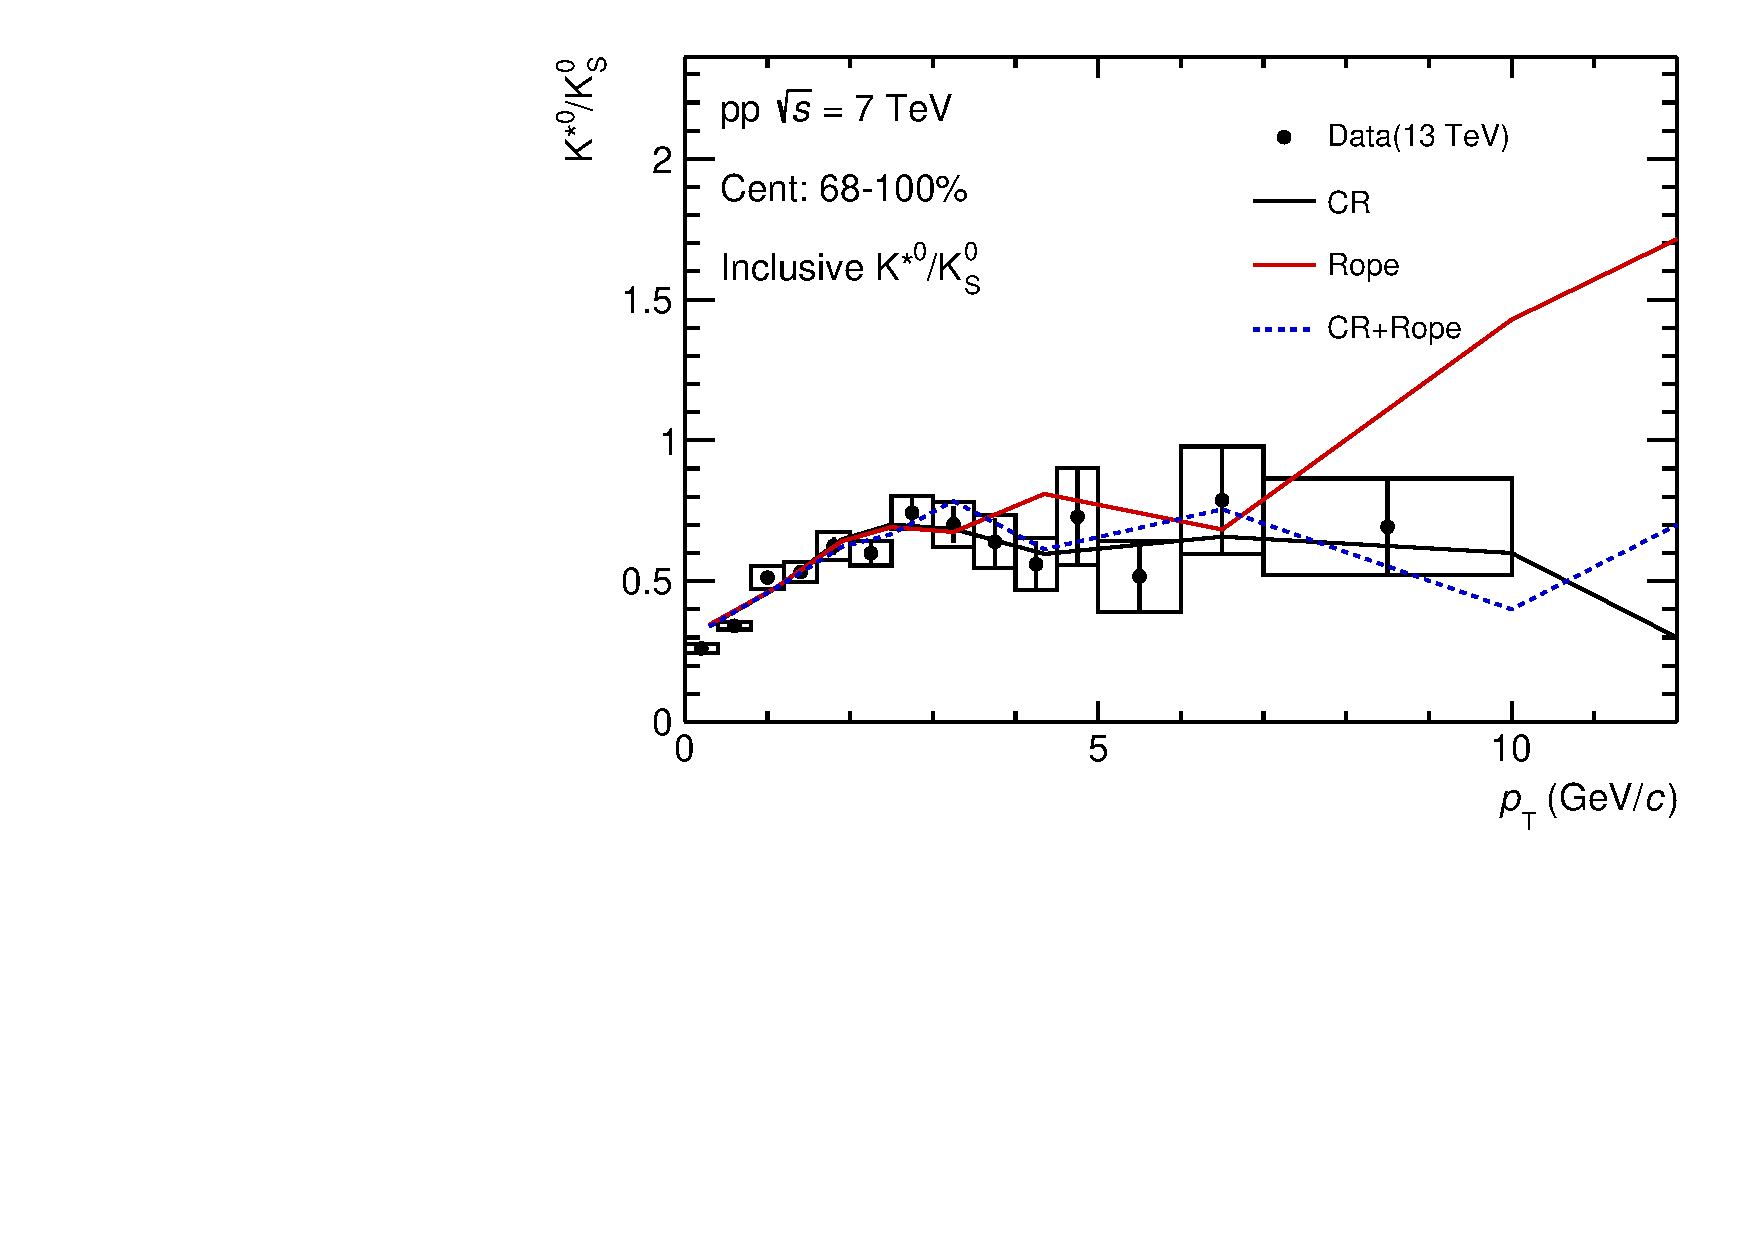
\includegraphics[width=.48\textwidth]{KstarKRatio_Incl_Peripheral}
%	\end{center}
%	\caption{Transverse momentum dependence of $\Lambda/\kzero$, $\phi/\kzero$ and $\kstar/\kzero$ yields ratios in \pp collisions at \seven for high (II) and low (X) multiplicity classes, respectively. Data taken from \cite{ALICE:2018pal, ALICE:2019etb}.}
%	\label{fig:InclParRatioCentPeri}
%\end{figure}

\clearpage
\section{Predictions}
\label{sec:predic}
In this work, we used CR, Rope and CR + Rope models to predict the particles produced in charged-particle jets distributions in \pp collisions at \seven. The analysis strategy is following the Ref~\cite{ALICE:2021cvd} which is studied the production of \kzero and \lmb in jets by ALICE experiment. The strange hadrons studied in this paper are generated within $|\eta| < 0.75$. The charged-particle jets are reconstructed using the \akT\ algorithm~\cite{Cacciari:2008gp} from the FastJet package~\cite{Cacciari:2011ma, Cacciari:2005hq}, which is a commonly used jet finding algorithm with resolution parameter $R = 0.4$. A cut on transverse momentum of reconstructed charged-particle jet ($\pTj > 10$~\GeVc) is applied according the ALICE study~\cite{ALICE:2021cvd}. To obtain the yields of hadrons within the charged-particle jet, the particles are selected based on their distance from the jet axis in the pseudo-rapidity and azimuthal angle plane~($\eta - \varphi$ plane)
\begin{equation}
	R(\mathrm{par, ~jet}) = \sqrt{\left( \eta_\mathrm{jet} - \eta_\mathrm{par} \right)^{2} + \left( \varphi_\mathrm{jet} - \varphi_\mathrm{par} \right)^{2}}.
\end{equation}
A particle with a radial distance from a given jet $R (\mathrm{par, ~jet}) < 0.4$ is considered matched to the charged-particle jets. The the particle yields are normalized to the density per unit area: $N_\mathrm{par}/(N_\mathrm{ev}A_\mathrm{acc})$. Where the $(N_\mathrm{ev}$ is the number of generated events which contain the selected charged-particle jets, the $A_\mathrm{acc}$ is the area of th acceptance in pseudo-rapidity and azimuthal angle. The $\pT$-integrated yield as a function of $\langle\dndeta\rangle_{|\eta| < 0.5}$, the ratio between particle $\pT$-integrated yields as a functions of $\langle\dndeta\rangle_{|\eta| < 0.5}$ , the $\pT$-differential yield and the ratio between particle $\pT$-differential yields will be studied in charged-particle jets in this section.

The $\pT$-integrated yields of \kzero, \kstar, $\phi$, $\lmb$, $\Xi$, and $\Omega$ as a function of $\avdndeta_{|\eta| < 0.5}$ in charged-particle jets distributions are presented in Figure~\ref{fig:JCIntePar}. It is shown that the $\pT$-integrated yields as a function of $\avdndeta_{|\eta| < 0.5}$ are not presented the increasing behavior which observed in inclusive cases.
%===================================================================
\begin{figure}[ht]
	\begin{center}
		%		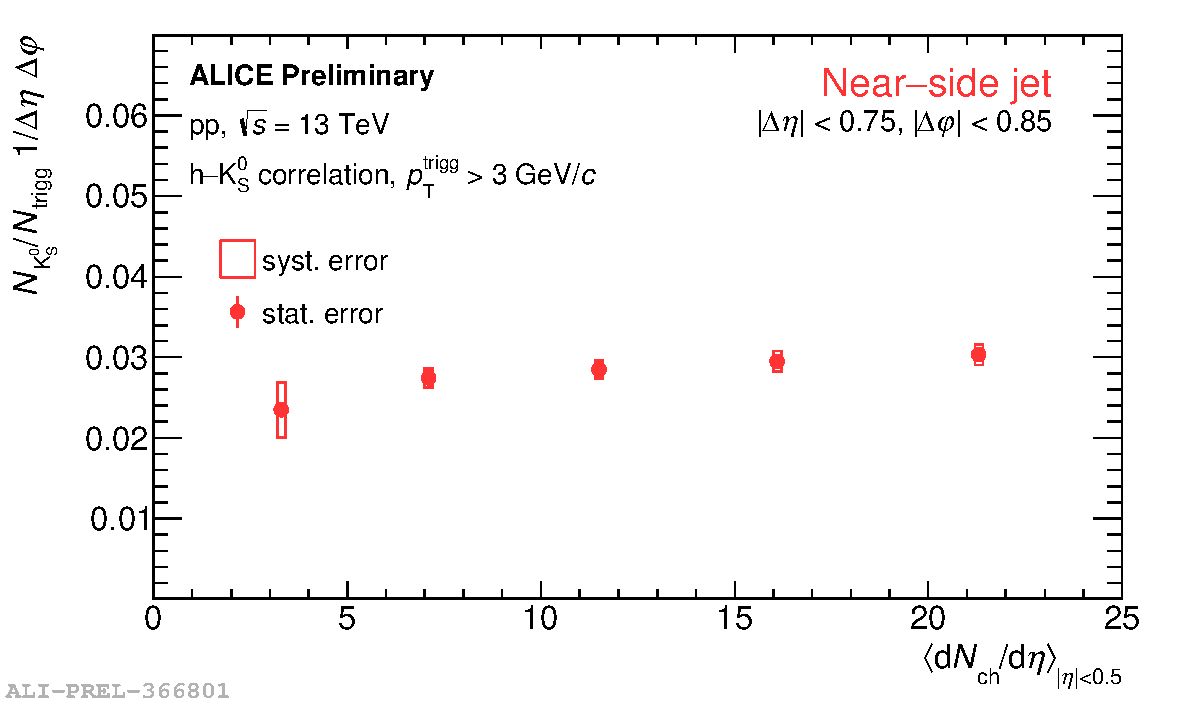
\includegraphics[width=.48\textwidth]{FinalYieldvsMultK0sJet_0}
		%		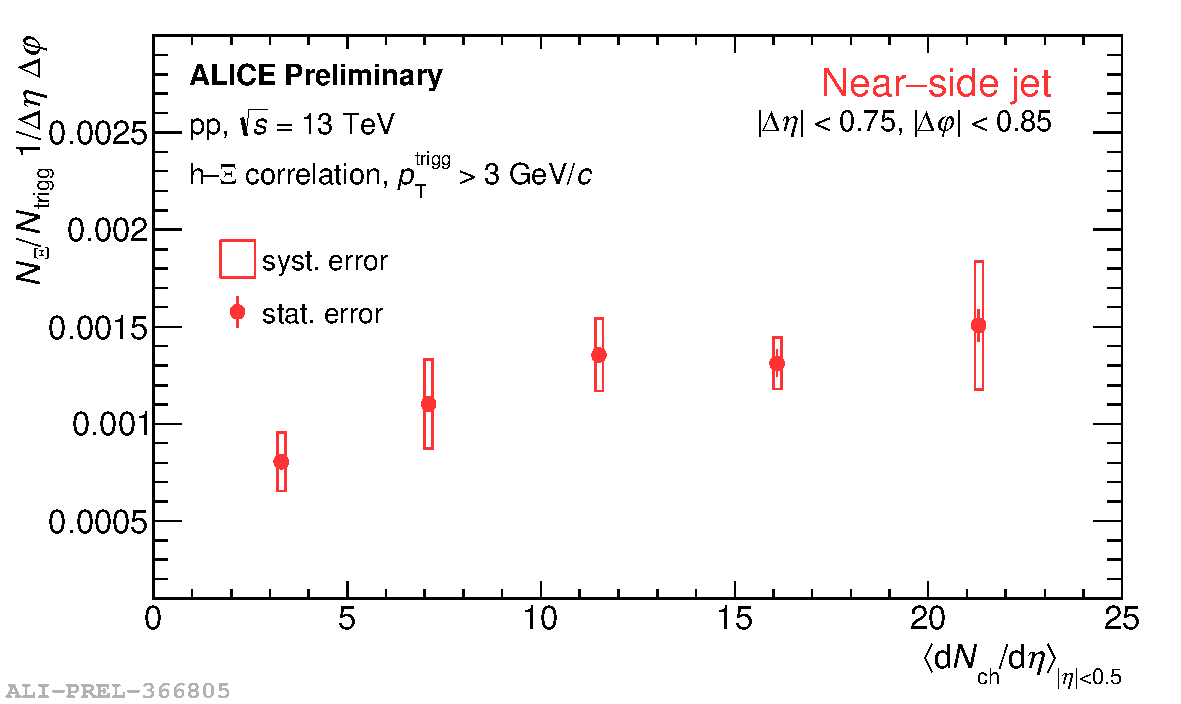
\includegraphics[width=.48\textwidth]{FinalYieldvsMultXiJet_0}
		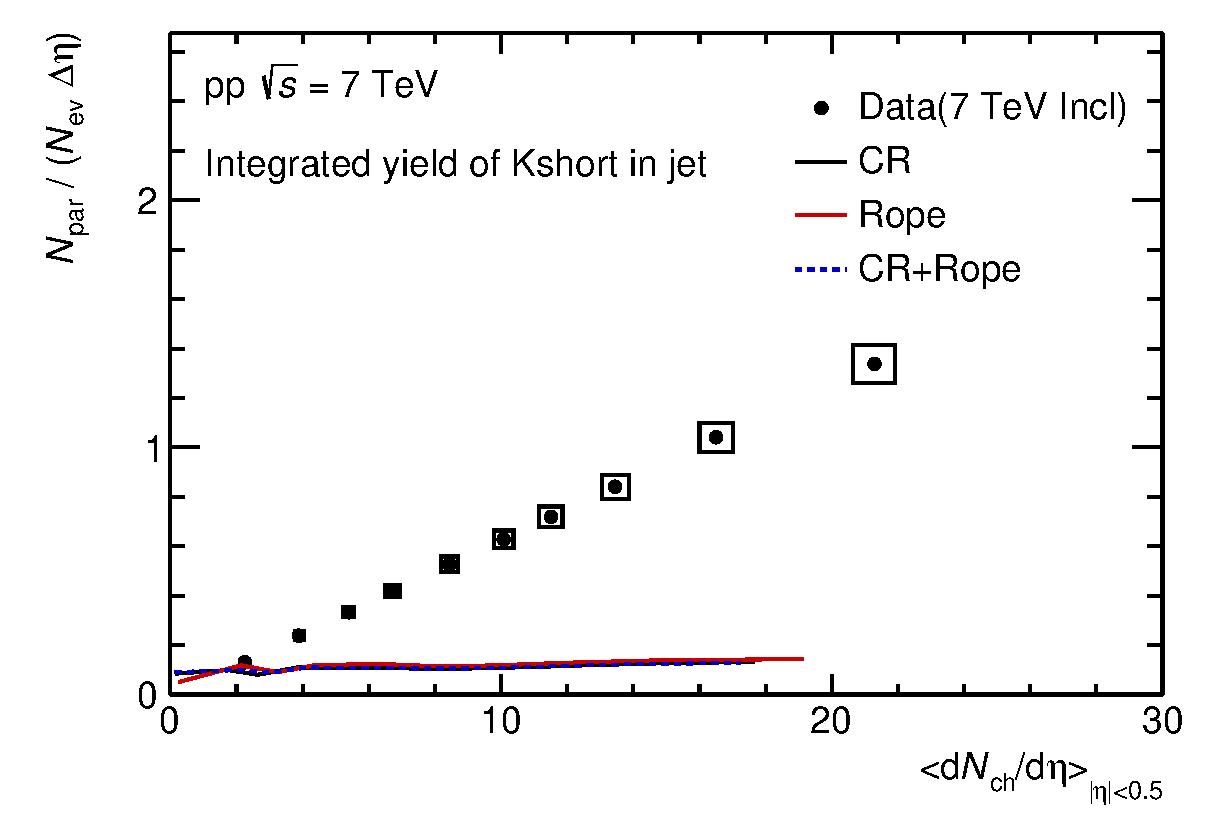
\includegraphics[width=.48\textwidth]{Kshort_InteSpectrum_JE}
		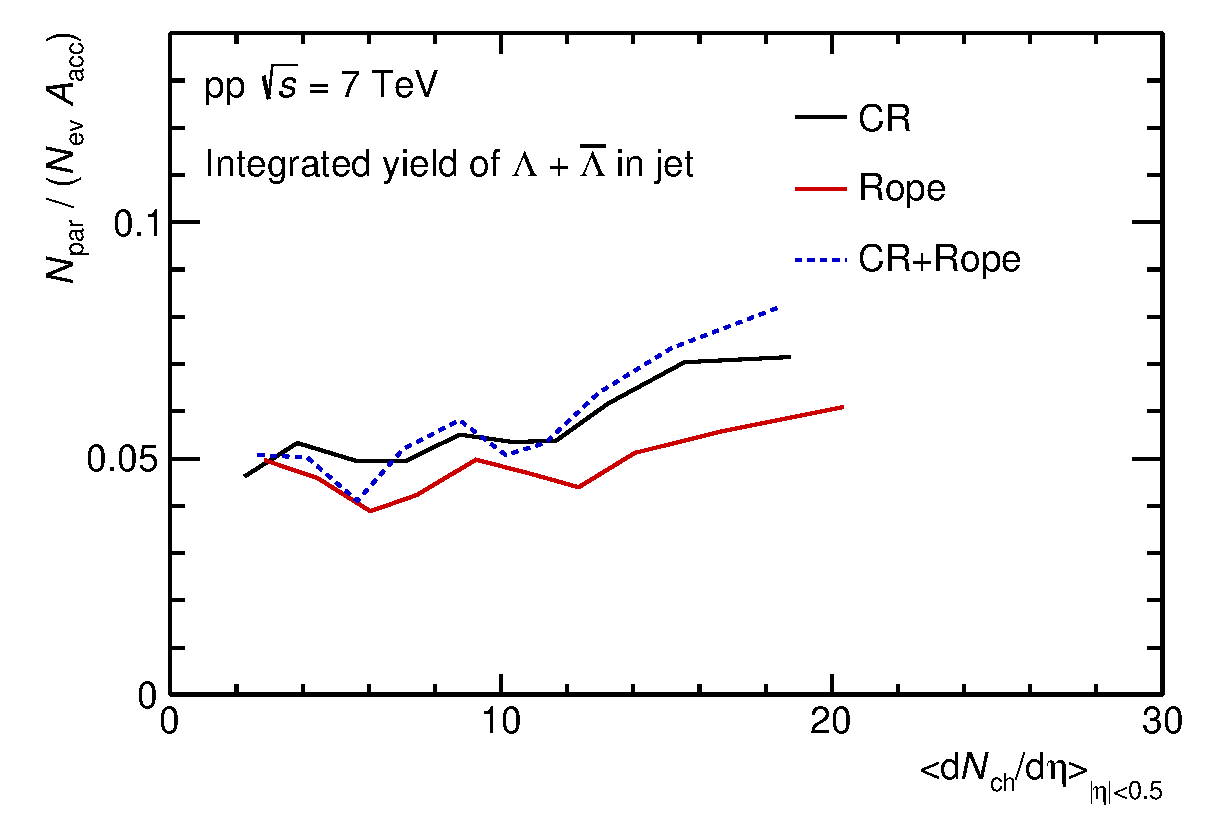
\includegraphics[width=.48\textwidth]{Lambda_InteSpectrum_JE}
		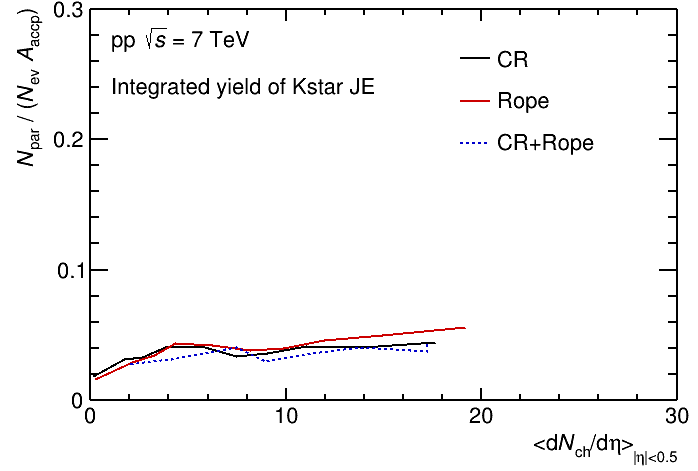
\includegraphics[width=.48\textwidth]{Kstar_InteSpectrum_JE}
		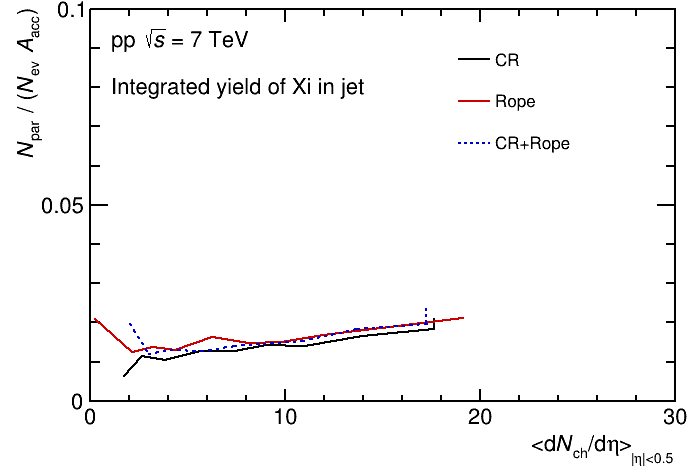
\includegraphics[width=.48\textwidth]{Xi_InteSpectrum_JE}
		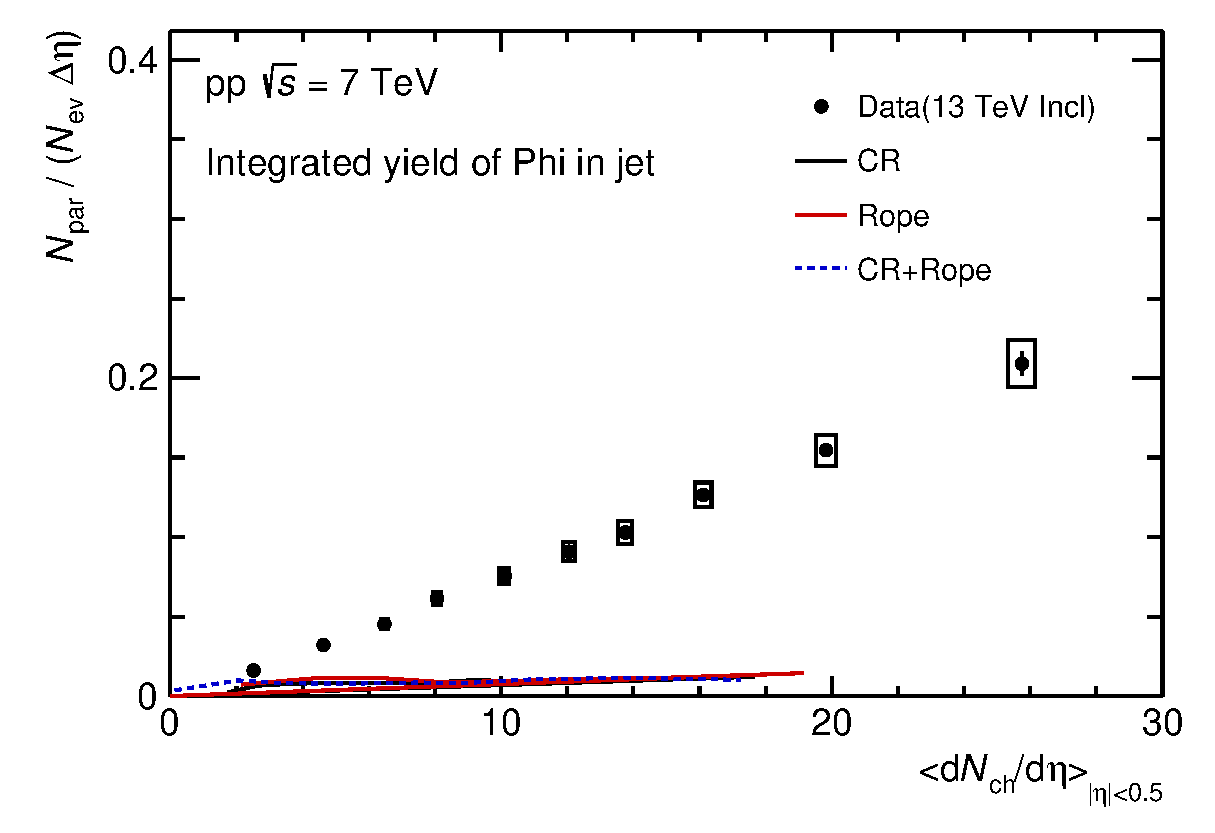
\includegraphics[width=.48\textwidth]{Phi_InteSpectrum_JE}
		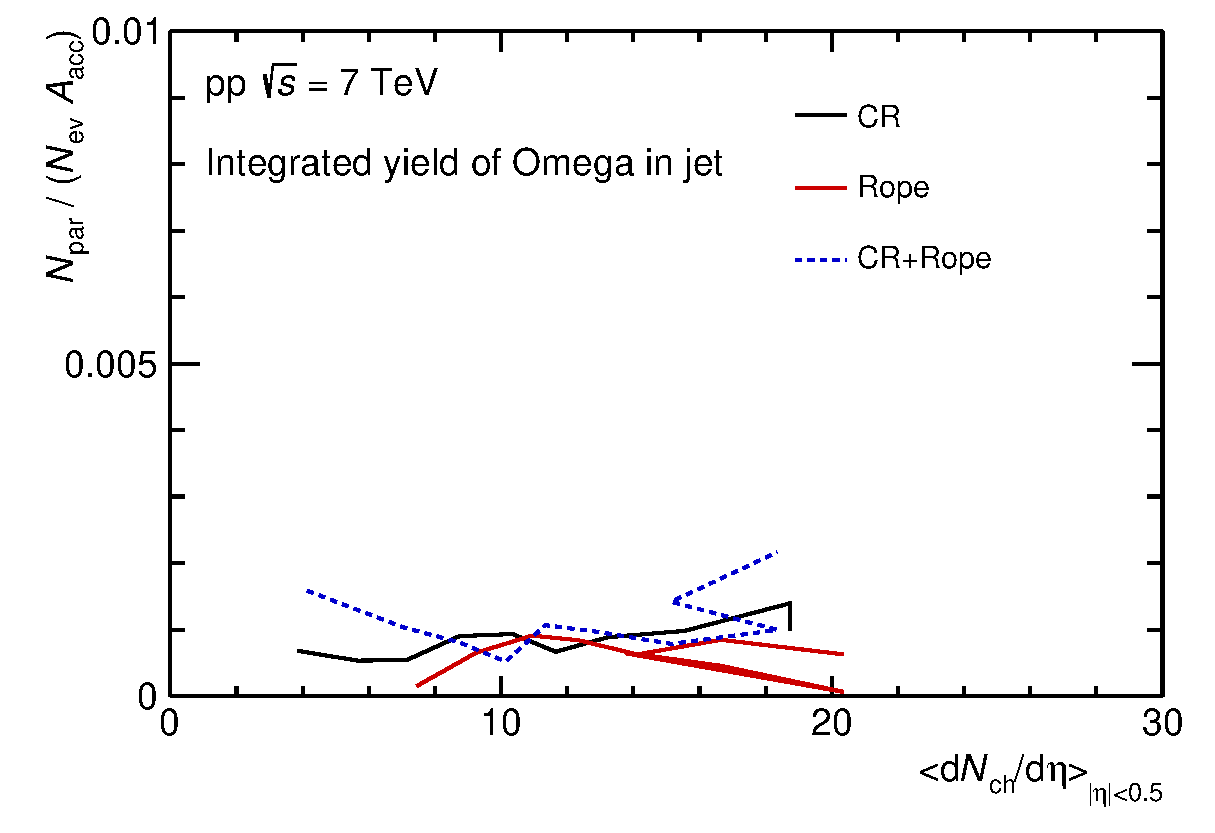
\includegraphics[width=.48\textwidth]{Omega_InteSpectrum_JE}
	\end{center}
	\caption{The $\pT$-integrated yields of \kzero, \kstar, $\phi$, $\lmb$, $\Xi$, and $\Omega$ in charged-particle jets as a function of $\avdndeta_{|\eta|<0.5}$ distributions.}
	\label{fig:JCIntePar}
\end{figure}

\begin{figure}[ht]
	\begin{center}
		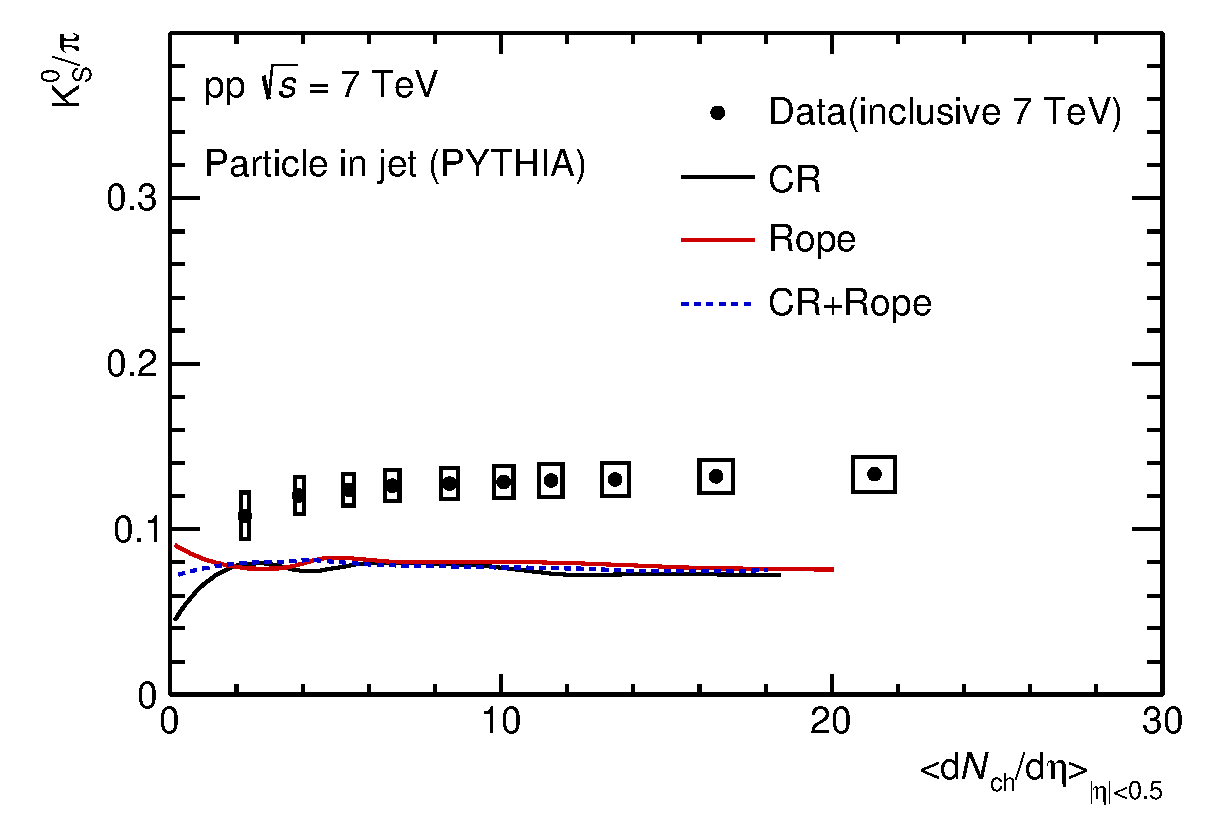
\includegraphics[width=.48\textwidth]{Kshort_PiRatio_JE}
		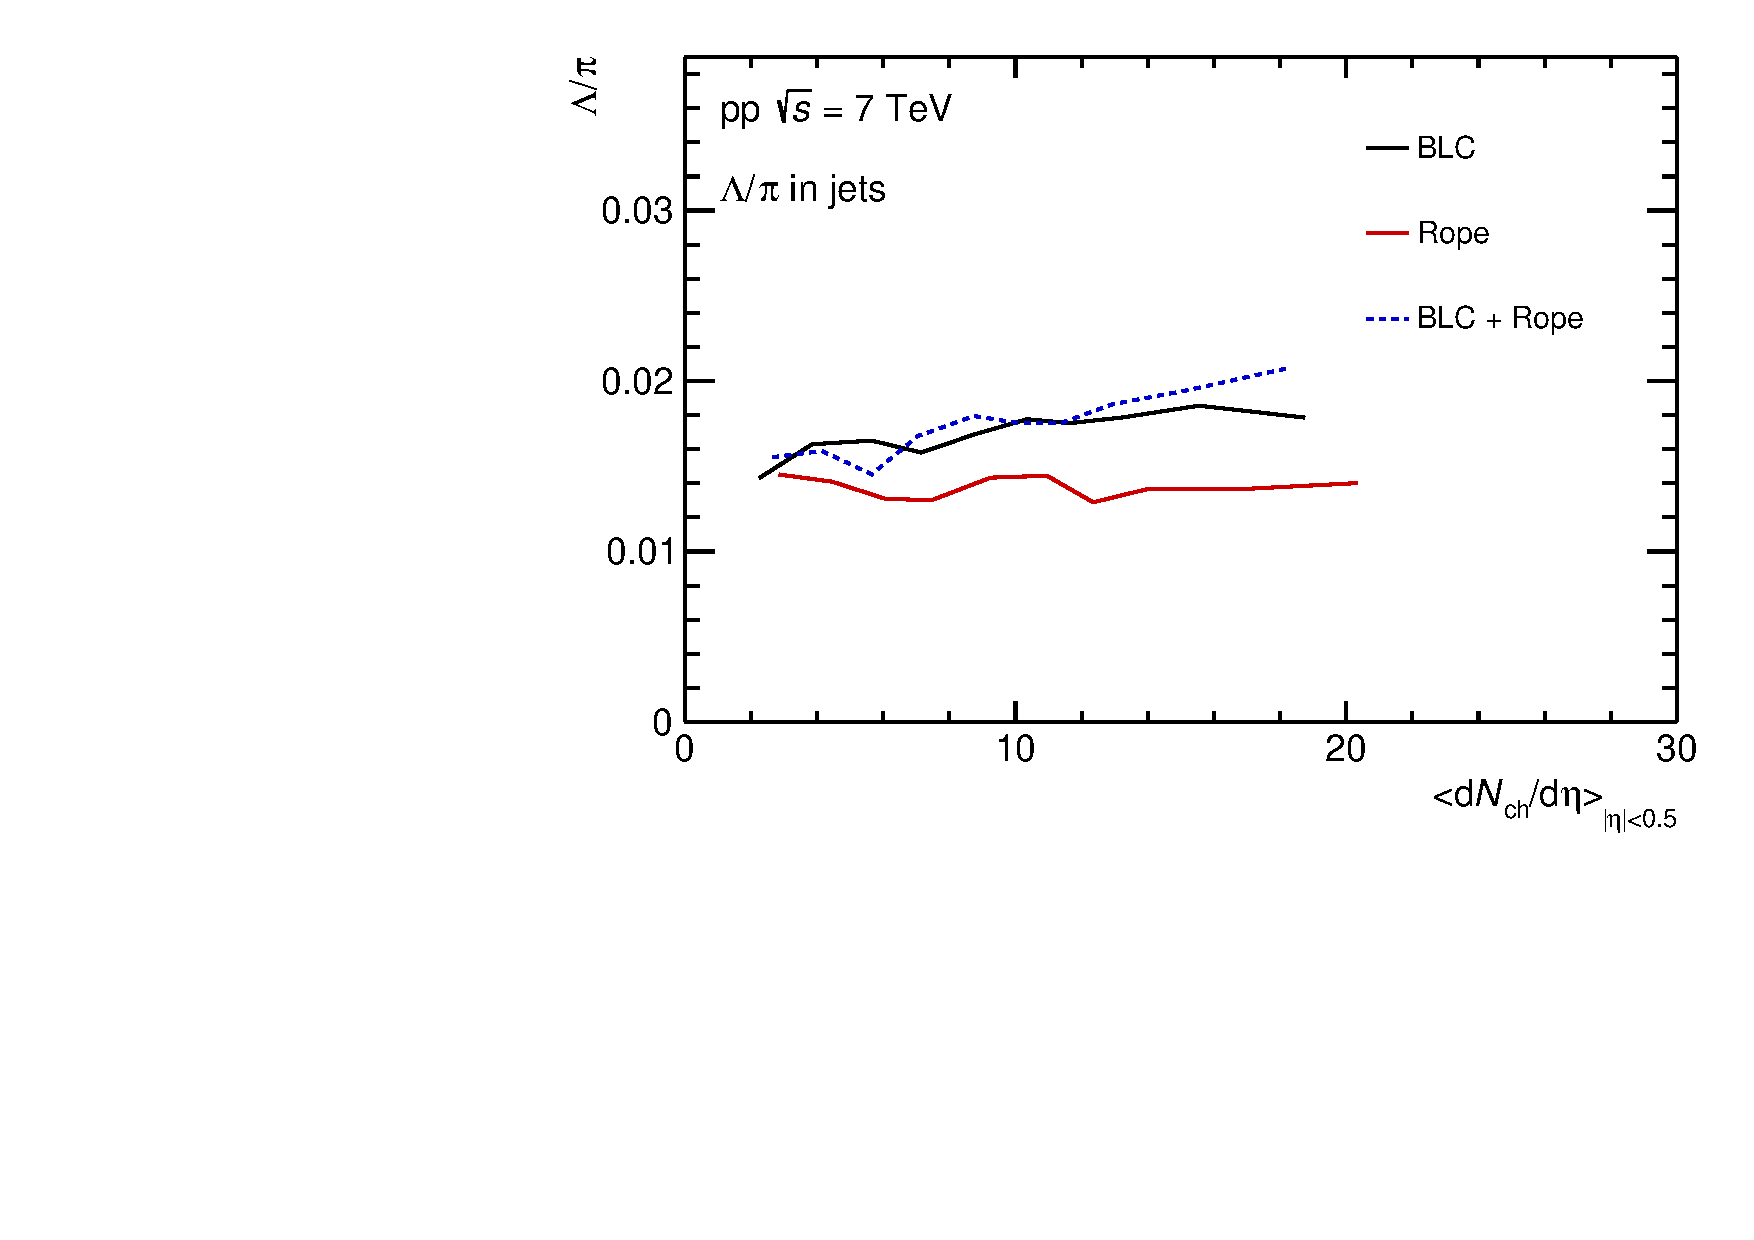
\includegraphics[width=.48\textwidth]{Lambda_PiRatio_JE}
		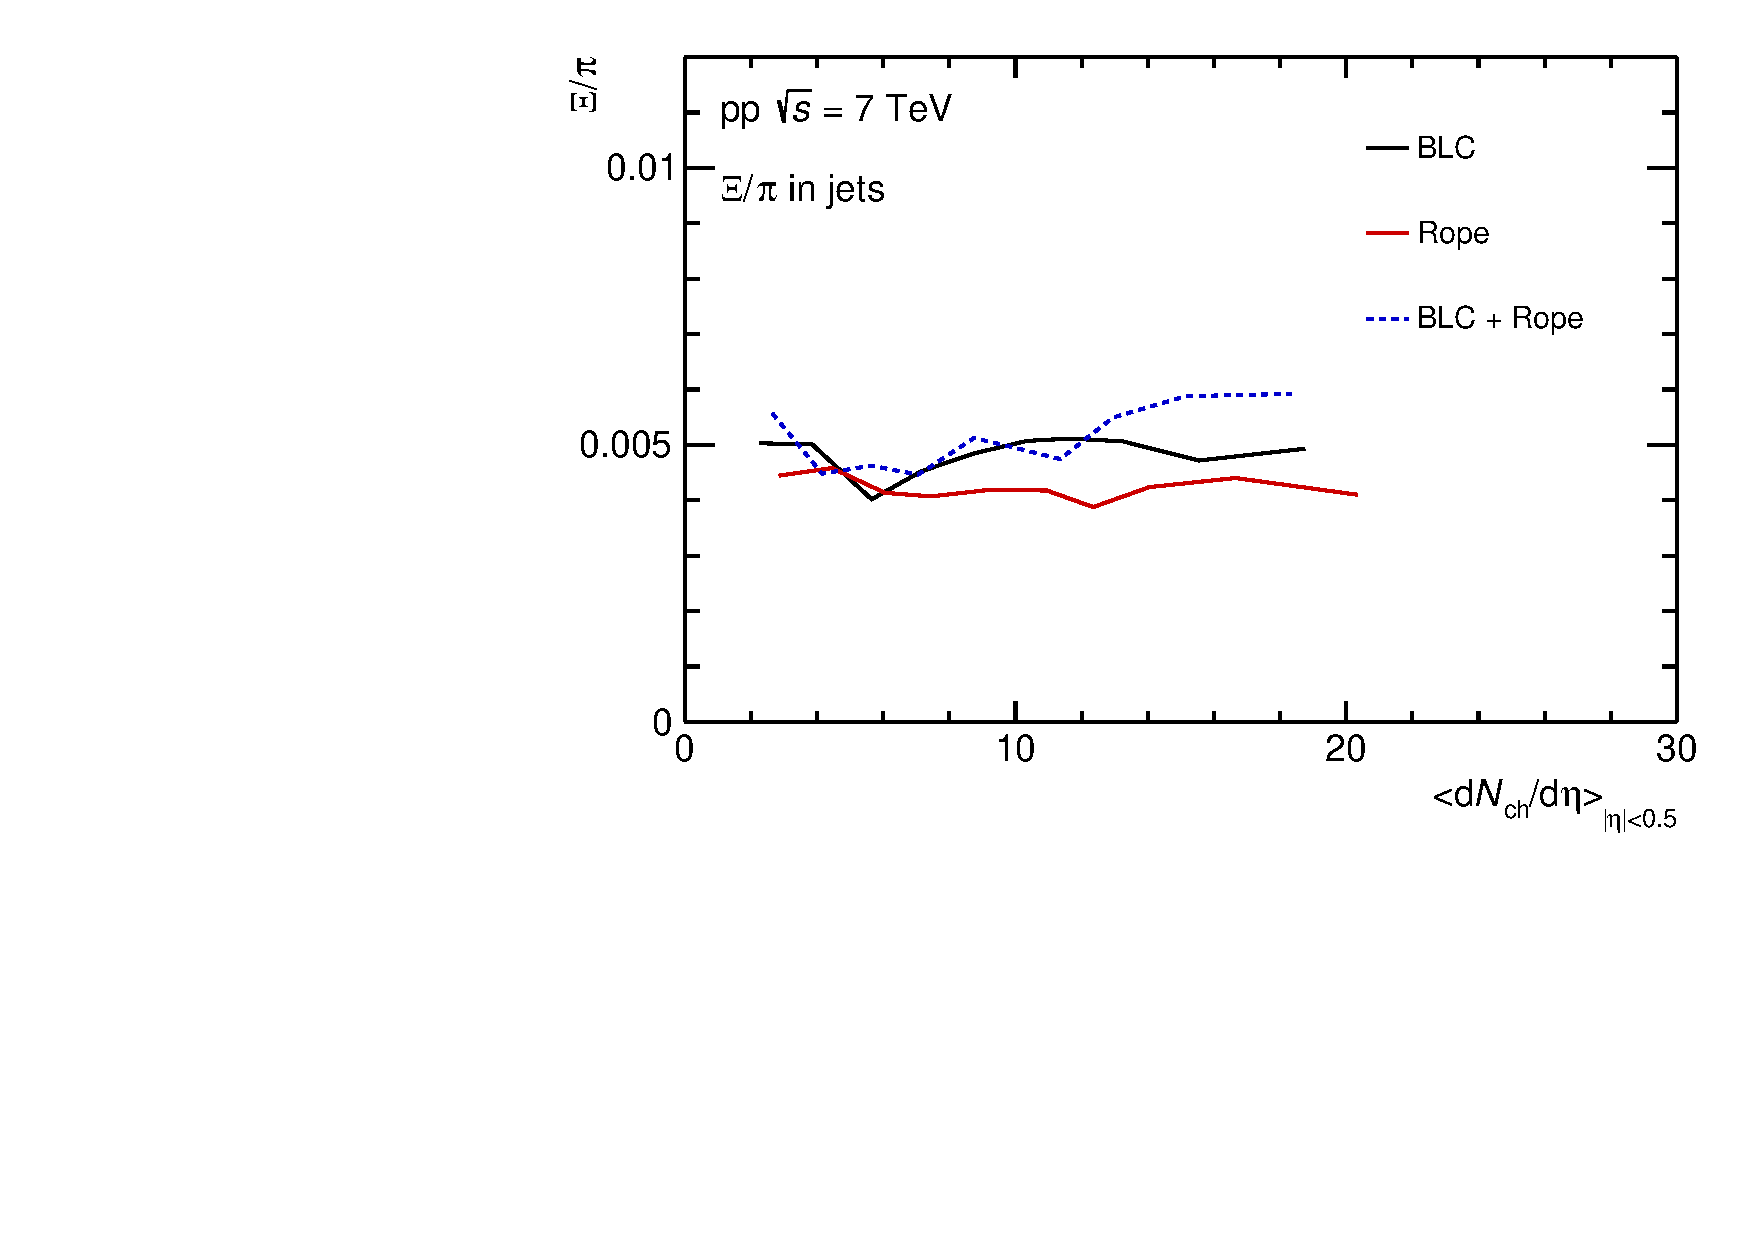
\includegraphics[width=.48\textwidth]{Xi_PiRatio_JE}
%		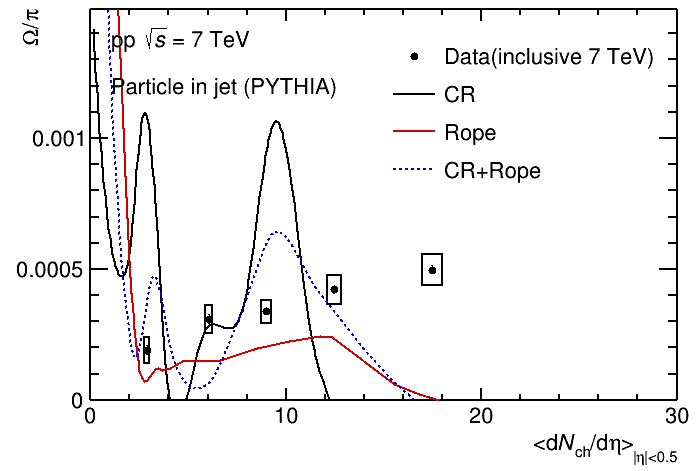
\includegraphics[width=.48\textwidth]{Omega_PiRatio_JE}
		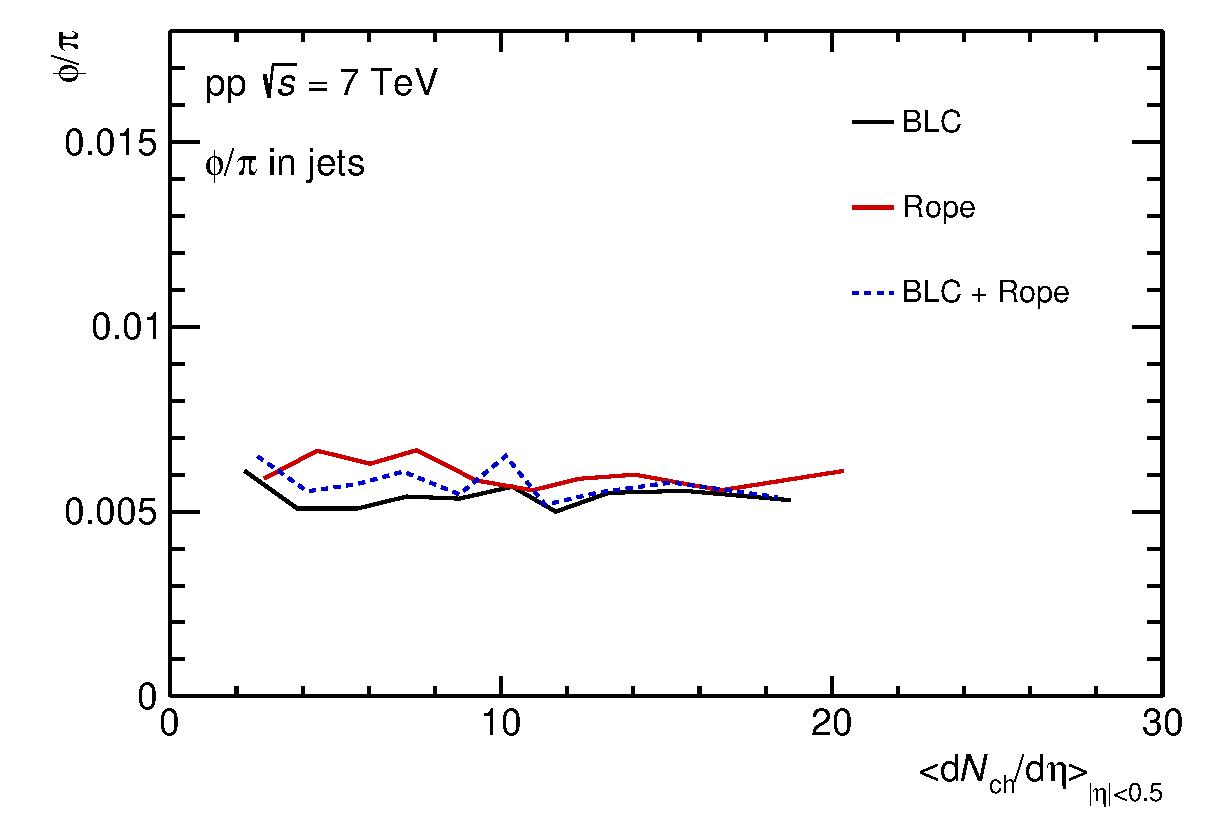
\includegraphics[width=.48\textwidth]{Phi_PiRatio_JE}
		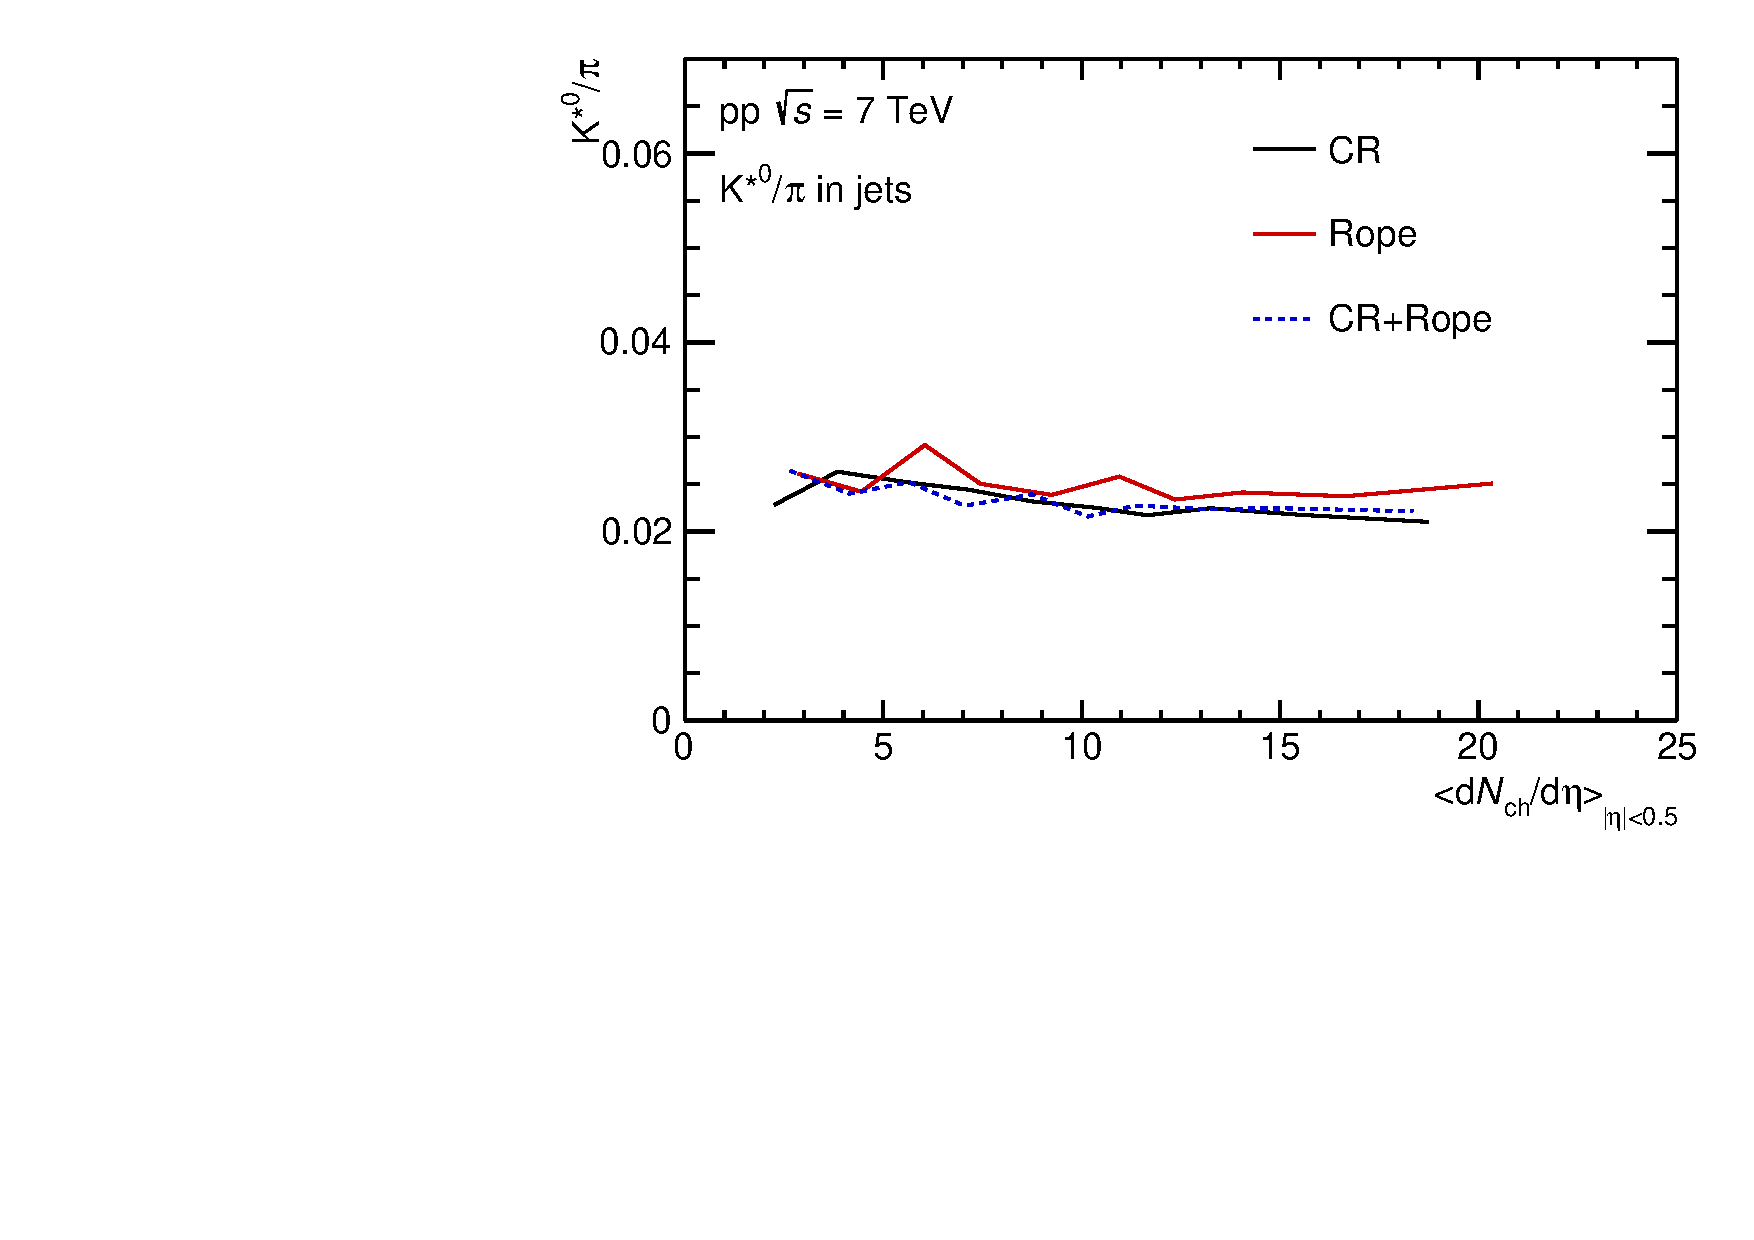
\includegraphics[width=.48\textwidth]{Kstar_PiRatio_JE}
	\end{center}
	\caption{Integrated yields ratios in jet of strange particle to $\pi$ with $\avdndeta_{|\eta|<0.5}$. (Data taken from arXiv:1606.07424v2 and arXiv:1807.11321v2)}
	\label{fig:JEIntePartoPiRatio}
\end{figure}


\begin{figure}[ht]
	\begin{center}
		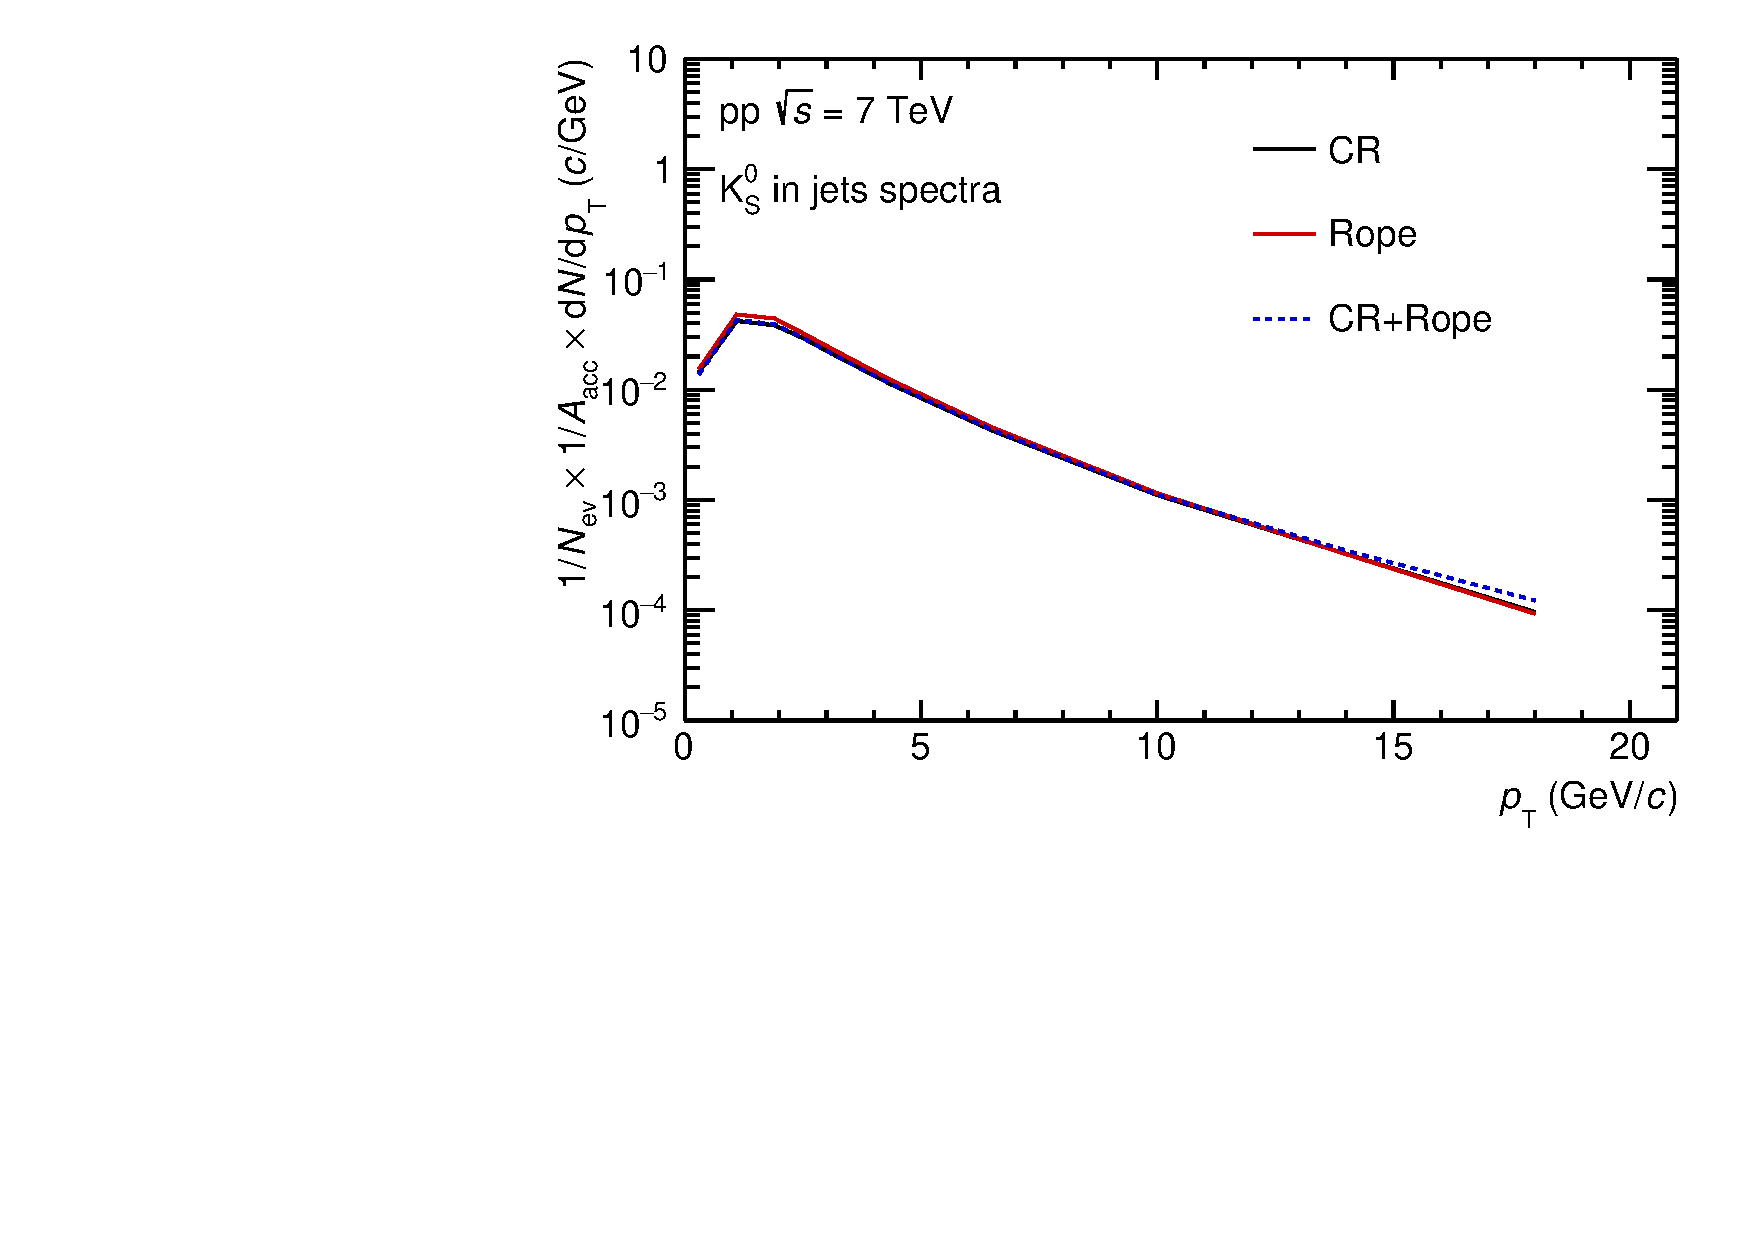
\includegraphics[width=.48\textwidth]{JE_KshortSpect}
		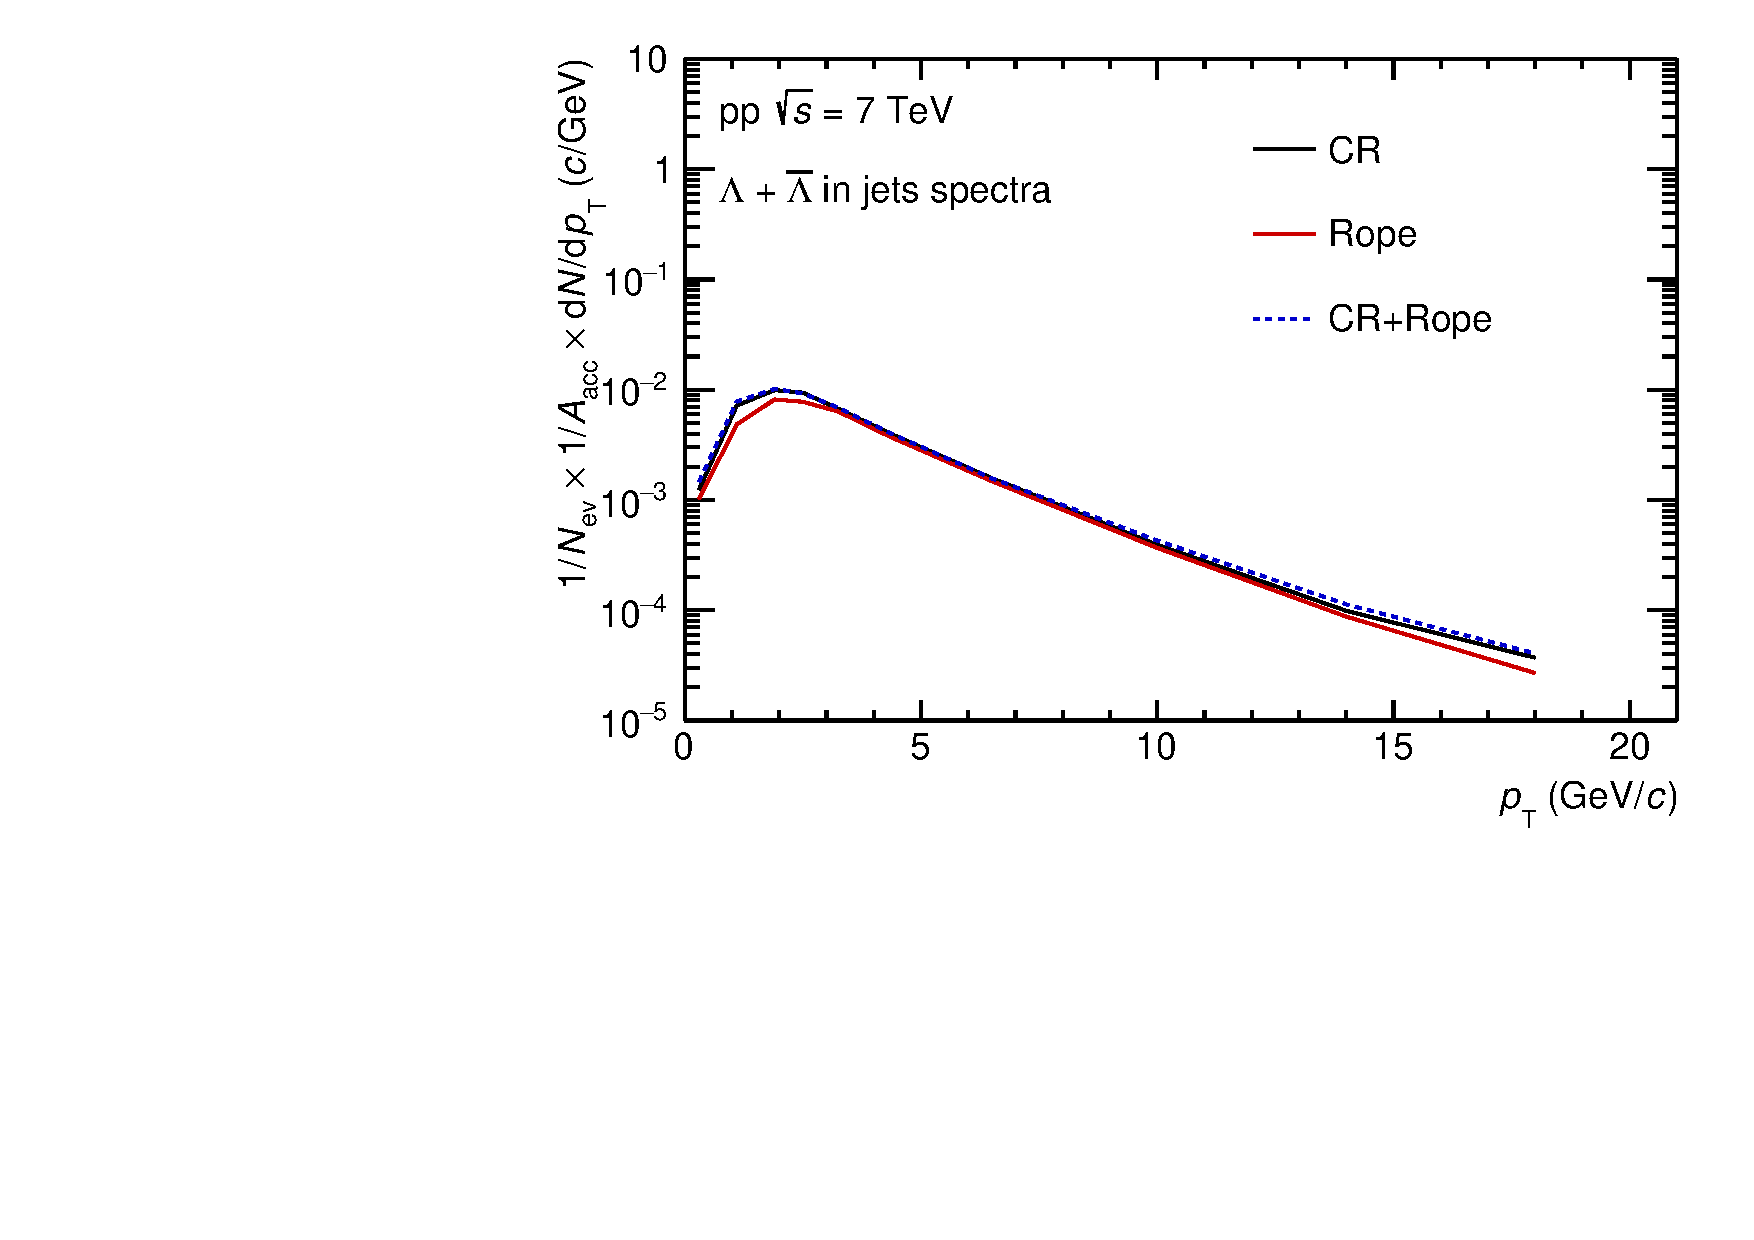
\includegraphics[width=.48\textwidth]{JE_LambdaSpect}
		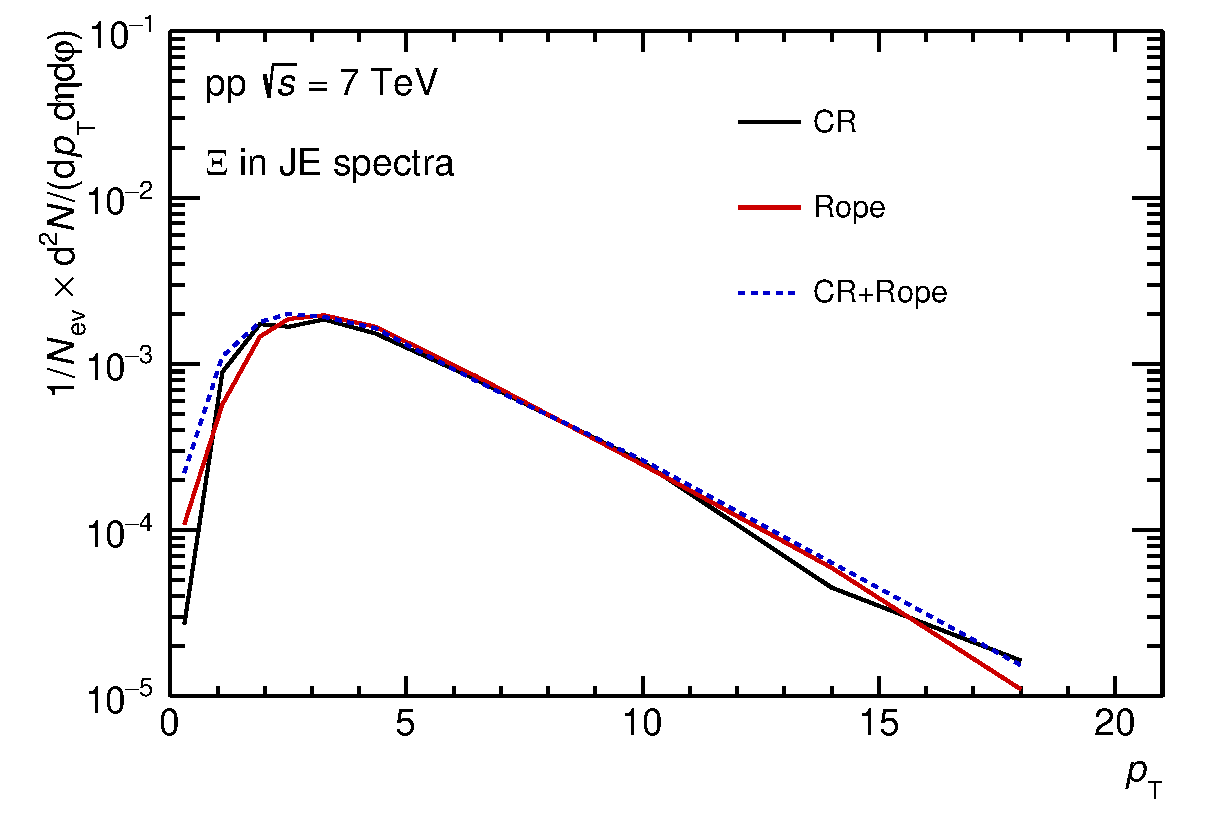
\includegraphics[width=.48\textwidth]{JE_XiSpect}
%		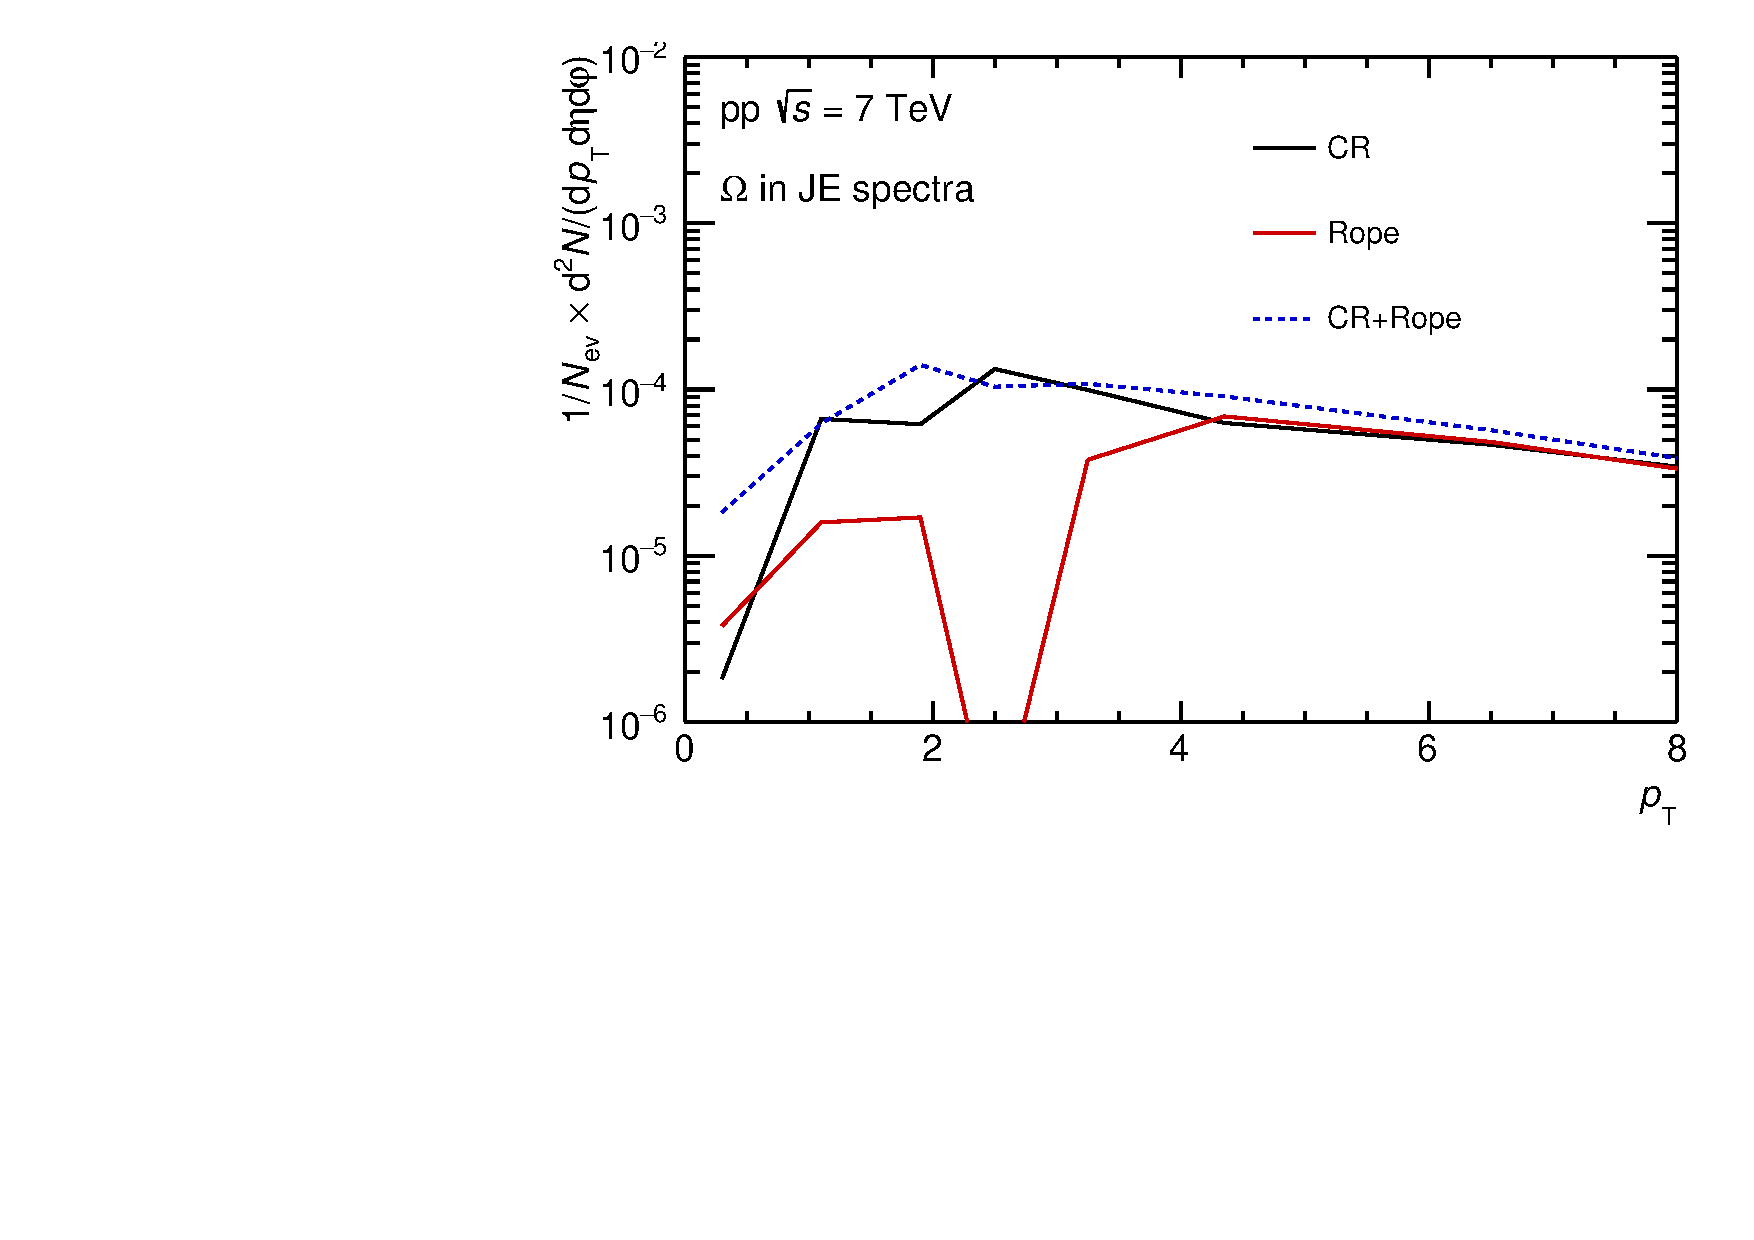
\includegraphics[width=.48\textwidth]{JE_OmegaSpect}
		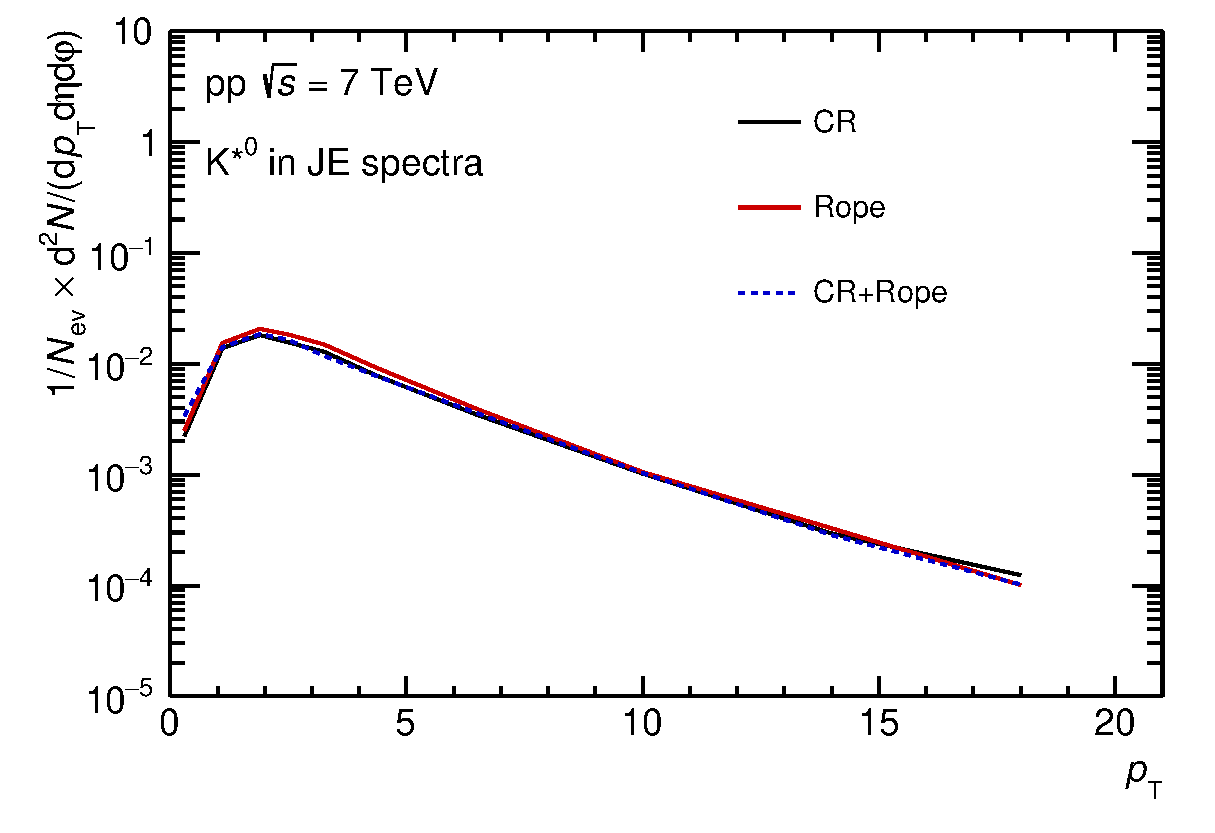
\includegraphics[width=.48\textwidth]{JE_KstarSpect}
		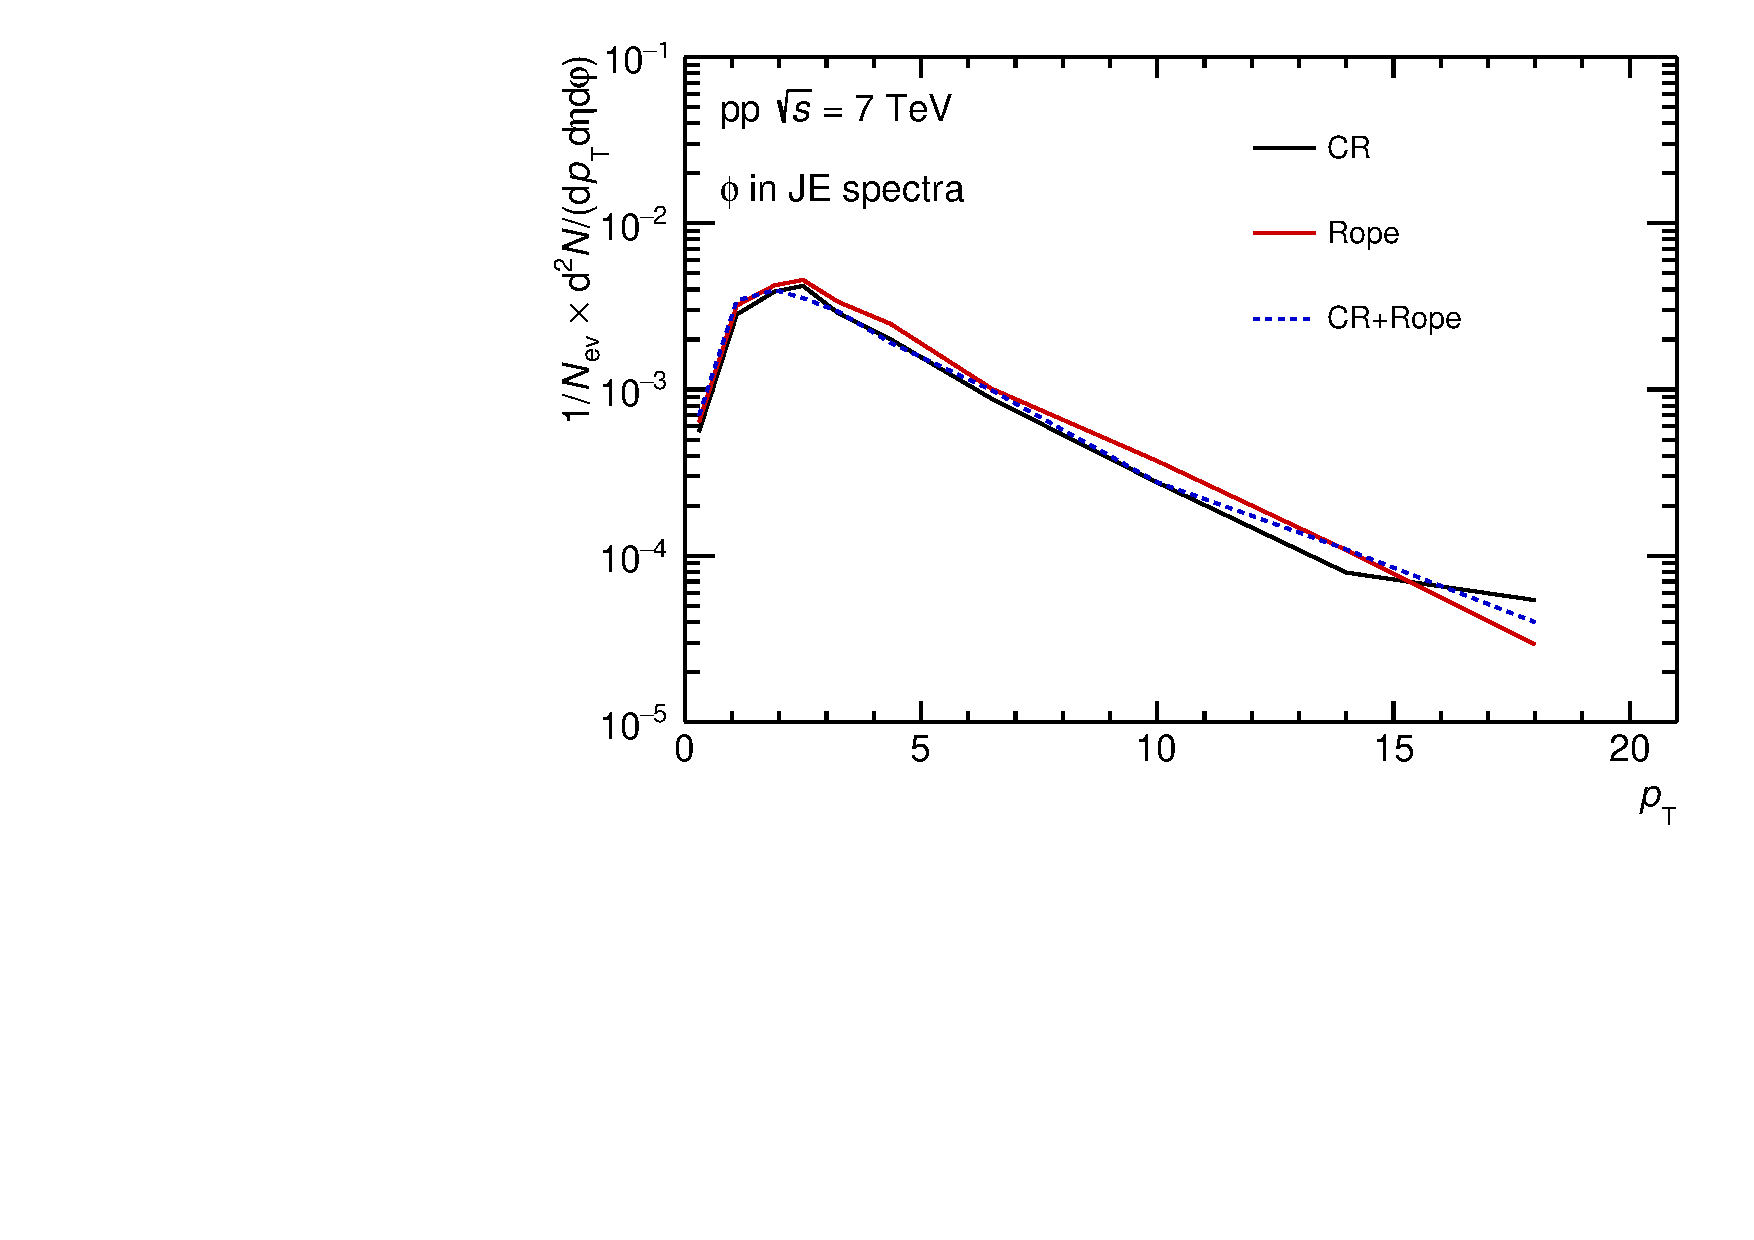
\includegraphics[width=.48\textwidth]{JE_PhiSpect}
	\end{center}
	\caption{Particle in jet $\pT$ spectra.}
	\label{fig:JEParSpect}
\end{figure}


\begin{figure}[ht]
	\begin{center}
		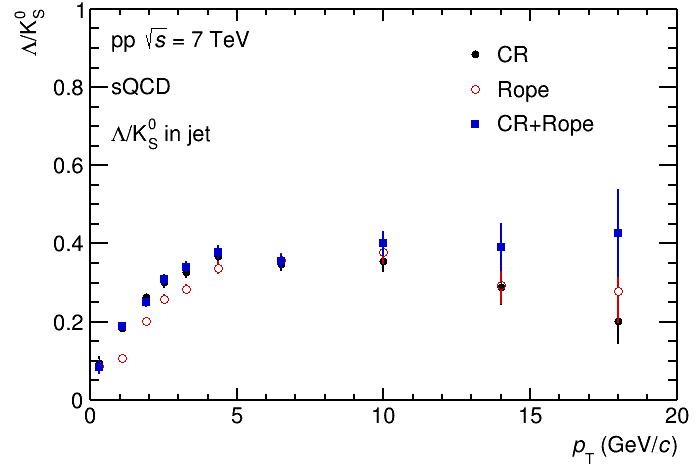
\includegraphics[width=.6\textwidth]{LKRatio_JE}
%		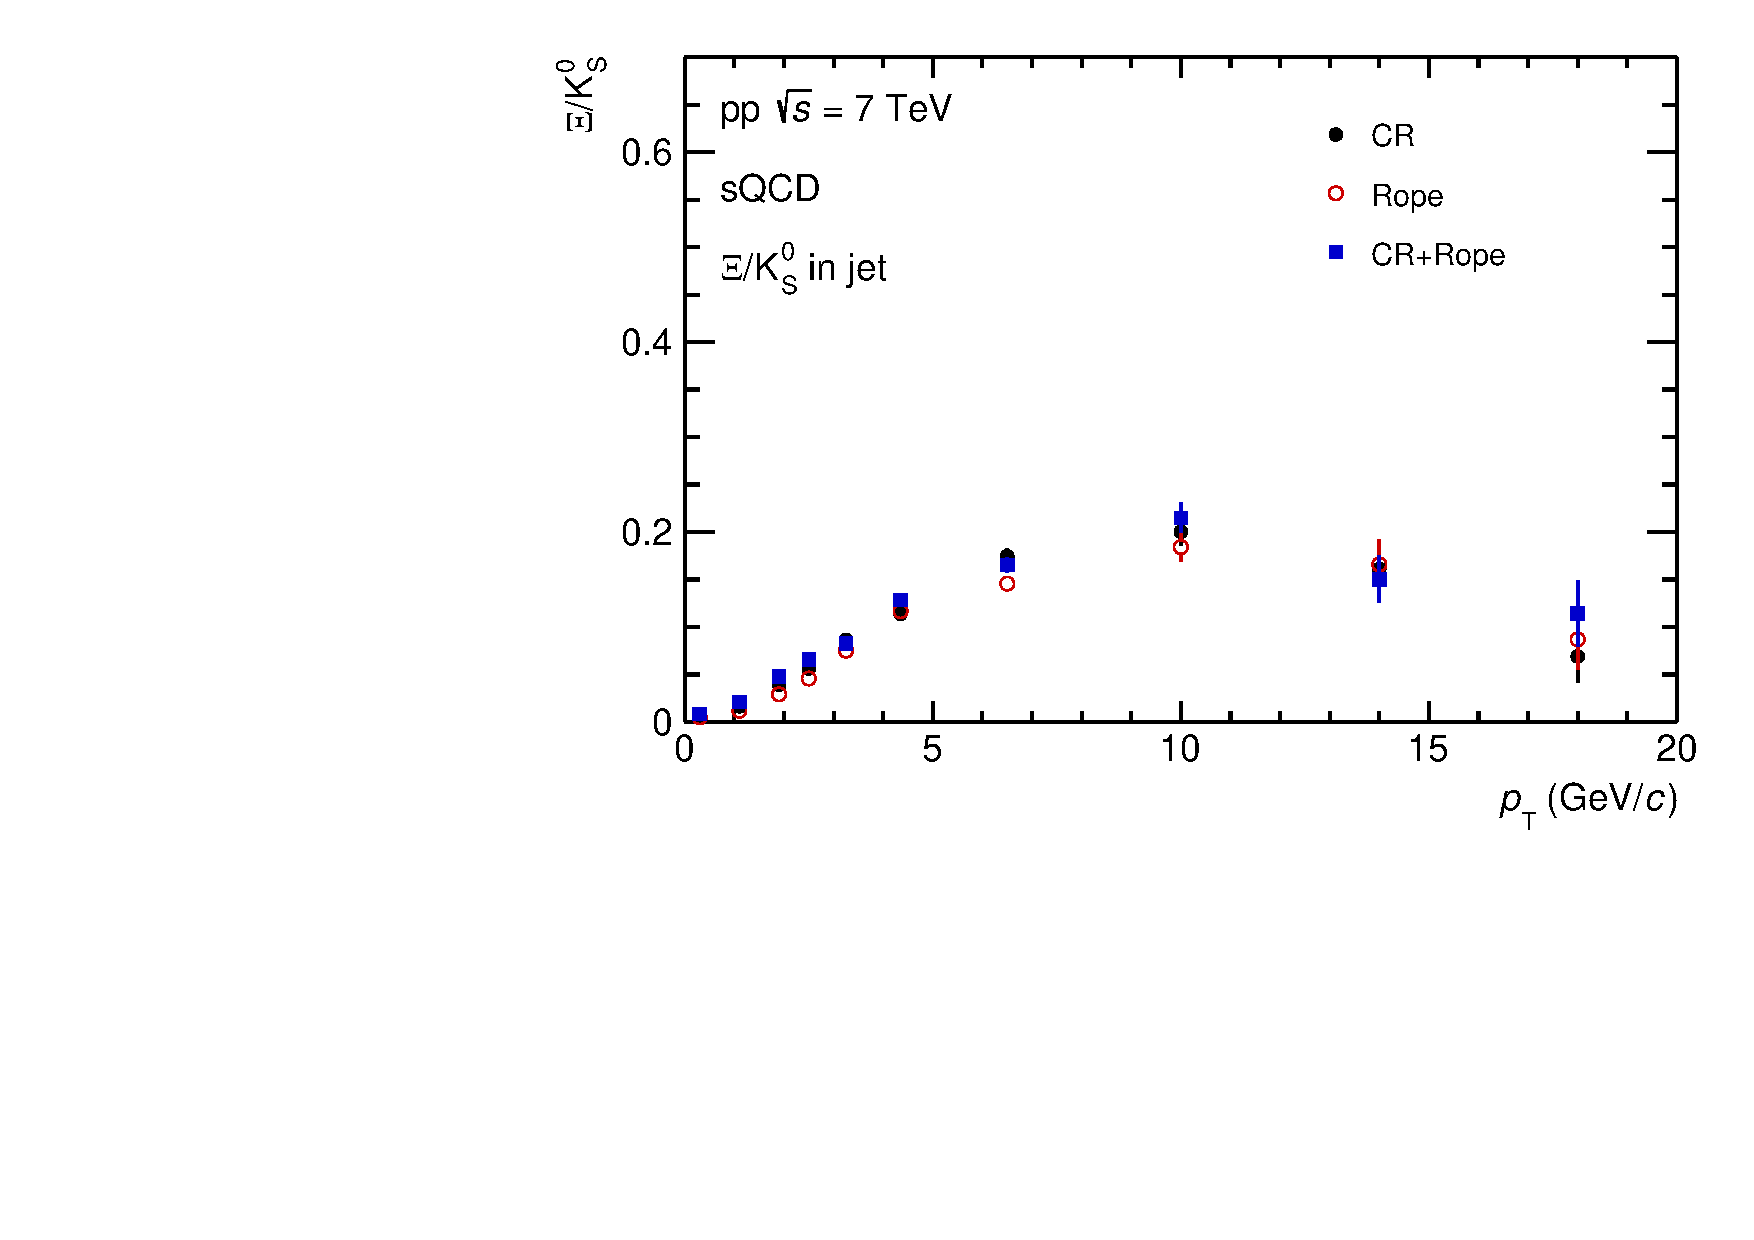
\includegraphics[width=.42\textwidth]{XKRatio_JE}
%		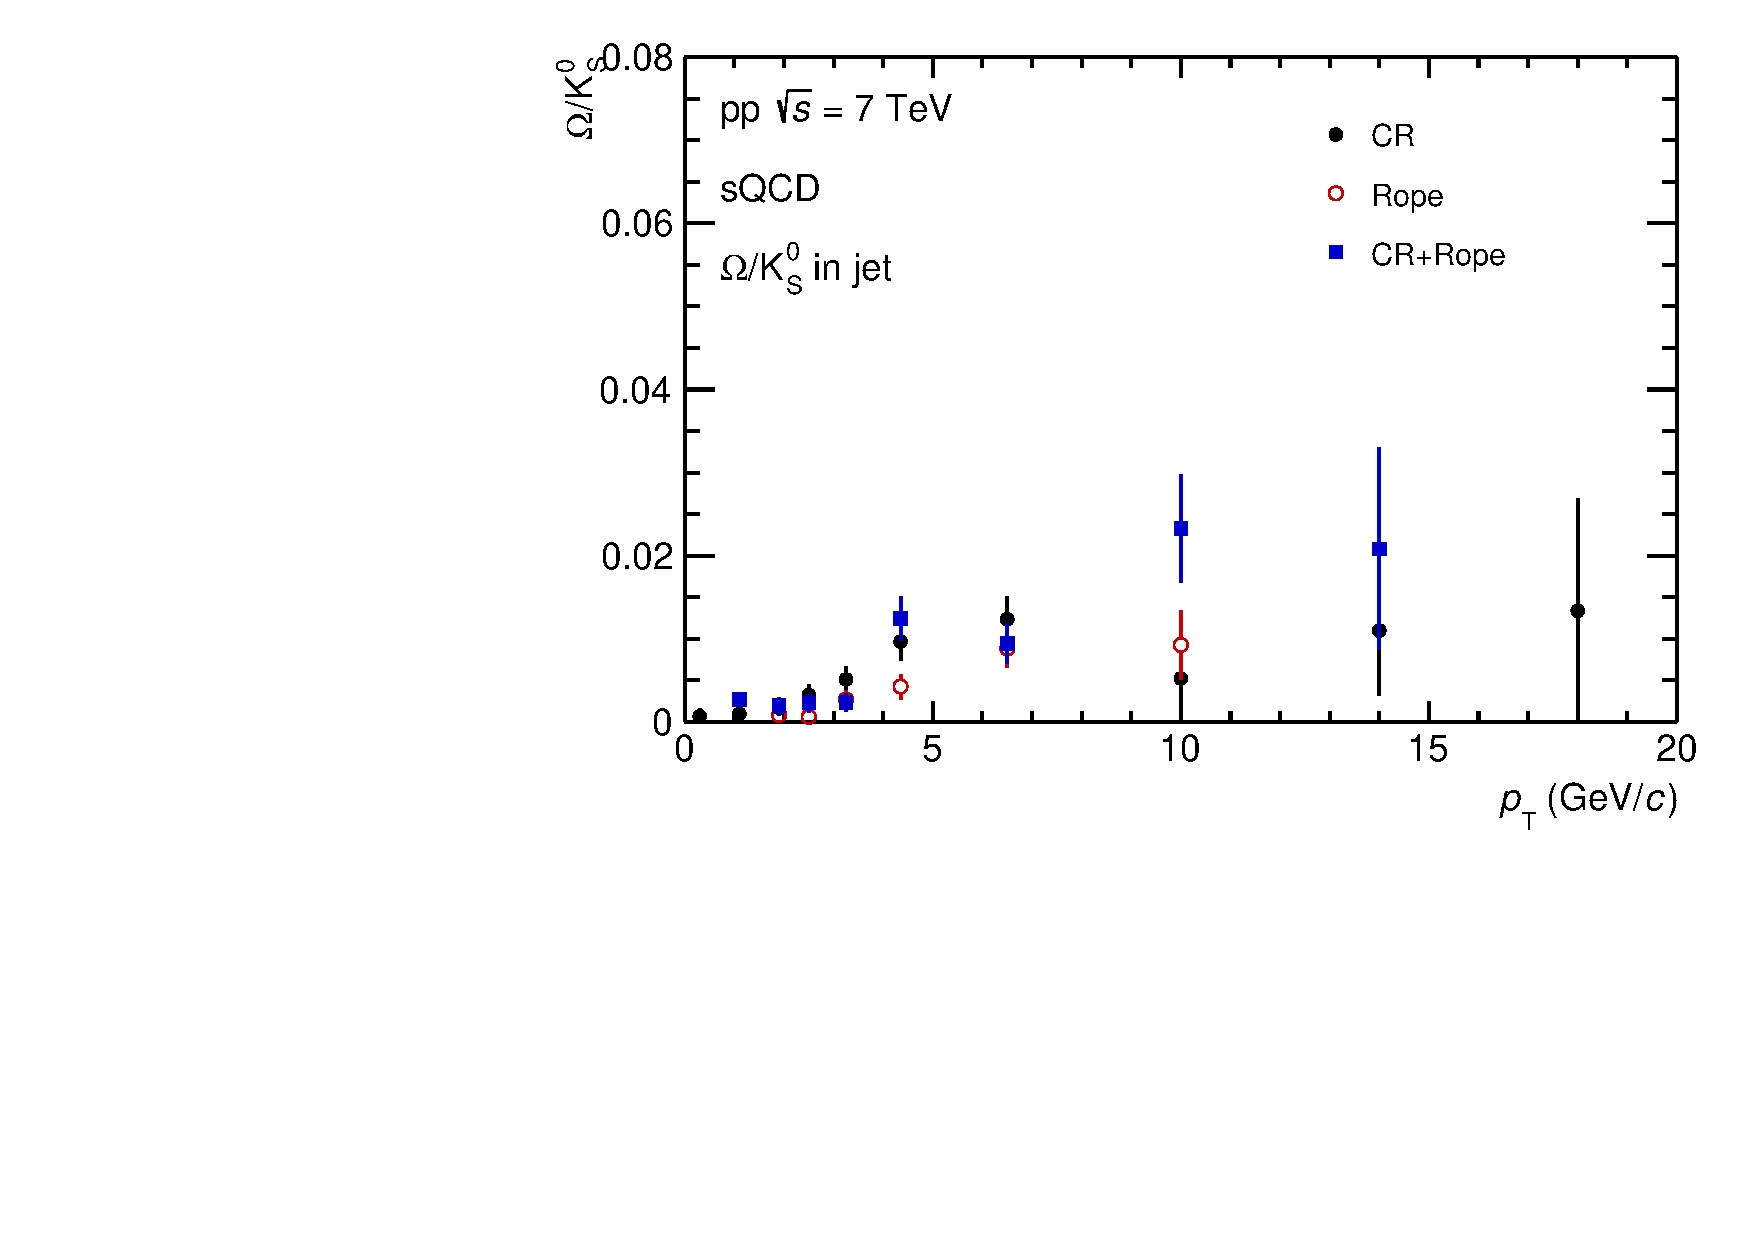
\includegraphics[width=.42\textwidth]{OKRatio_JE}
%		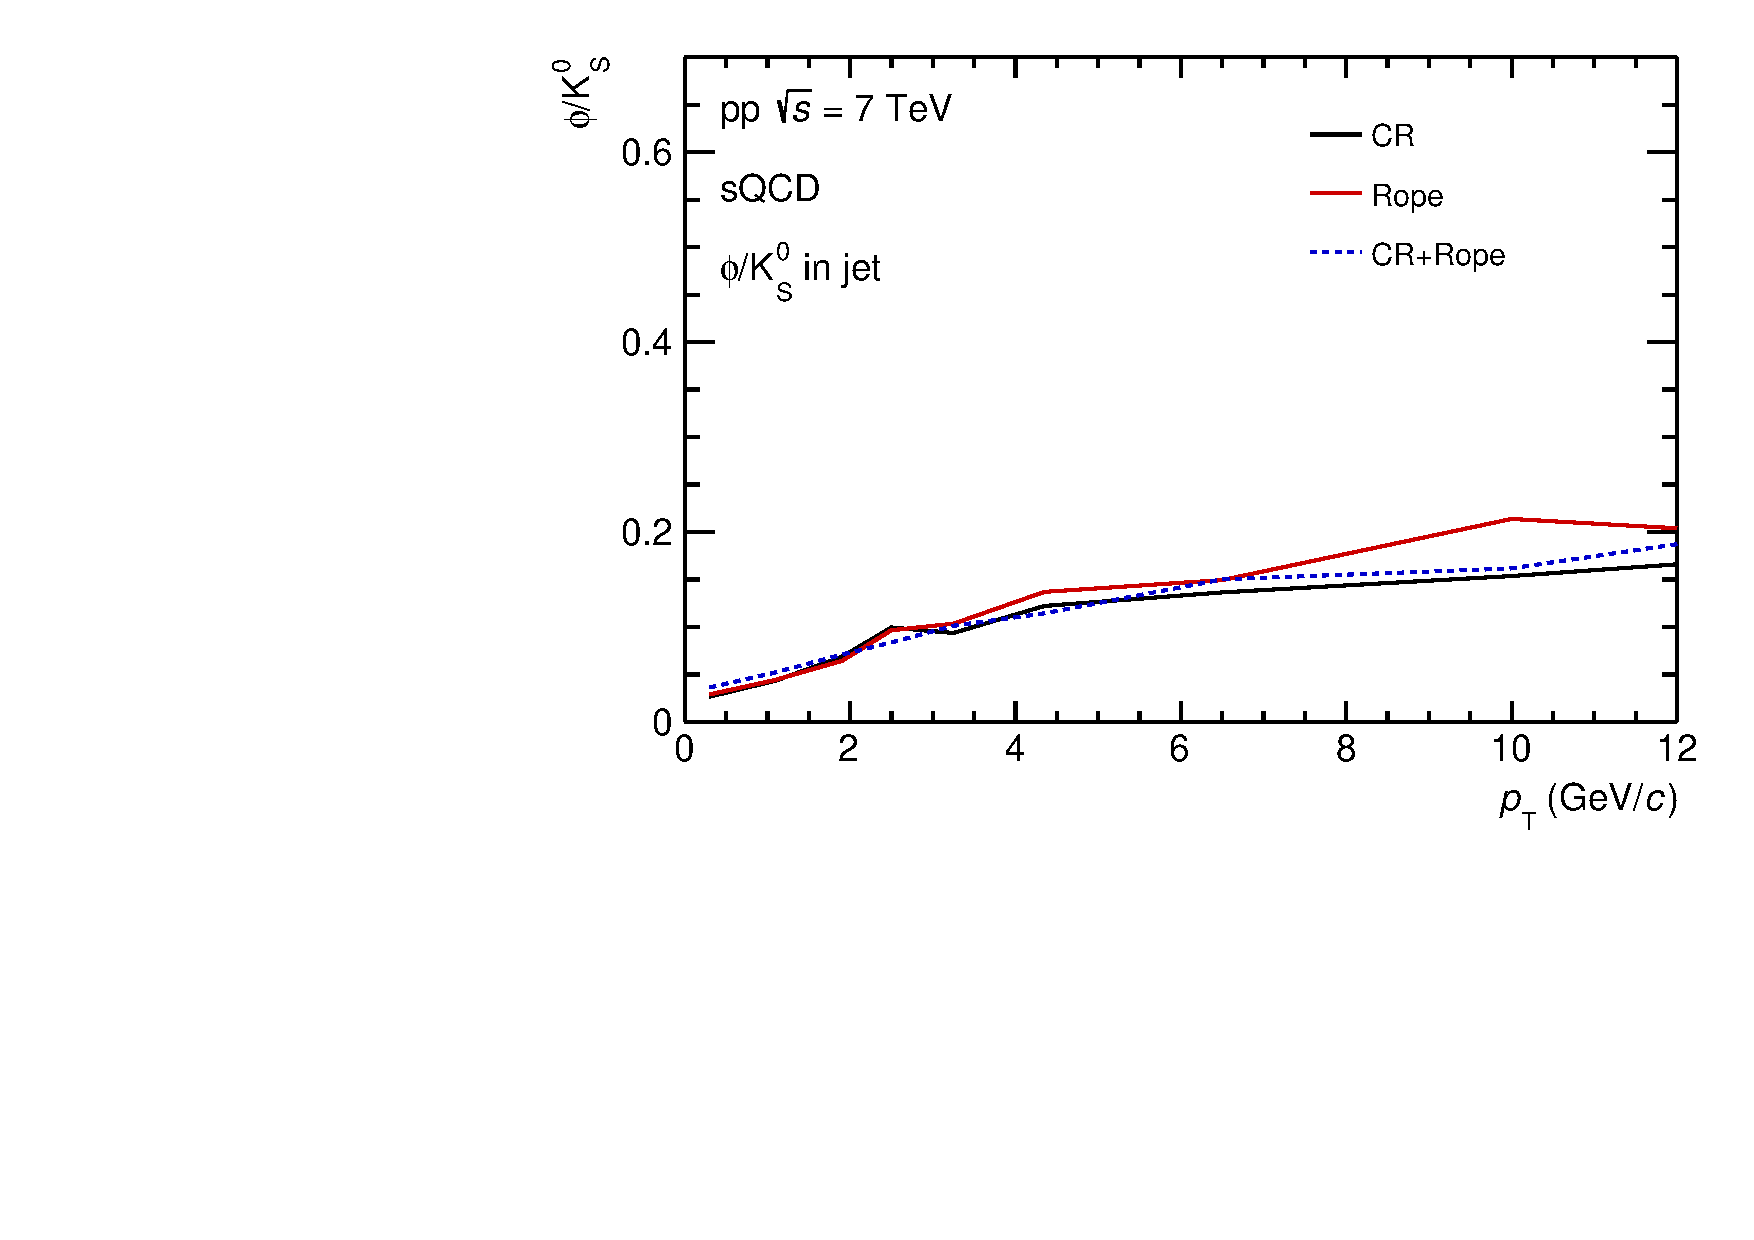
\includegraphics[width=.42\textwidth]{PhiKRatio_JE}
%		\includegraphics[width=.42\textwidth]{KstarKRatio_JE}
%		\includegraphics[width=.42\textwidth]{XLRatio_JE}
%		\includegraphics[width=.42\textwidth]{OLRatio_JE}
%		\includegraphics[width=.42\textwidth]{OXRatio_JE}
%		\includegraphics[width=.42\textwidth]{XPhiRatio_JE}
%		\includegraphics[width=.42\textwidth]{OPhiRatio_JE}
		%\includegraphics[width=.32\textwidth]{ProtonPionRatio_Incl}
	\end{center}
	\caption{Particle ratios in jet with $\pT$ distribution. (Data taken from arXiv:2005.11120)}
	\label{fig:JEParRatio}
\end{figure}


\begin{figure}[ht]
	\begin{center}
		\includegraphics[width=.42\textwidth]{LKRatio_JE_Cent_cr_rope}
		\includegraphics[width=.42\textwidth]{LKRatio_JE_Cent_cr}
		\includegraphics[width=.42\textwidth]{LKRatio_JE_Cent_rope}

	\end{center}
	\caption{Particle ratios in jet with $\pT$ distribution in different centrality bins.}
	\label{fig:JEParRatioCent}
\end{figure}

%\begin{figure}[ht]
%	\begin{center}
%		\includegraphics[width=.42\textwidth]{LK_toJetRange}
%	\end{center}
%	\caption{Particle ratios to jet axis range ($R$(P, jet)) distribution. (The multi-strange hadrons ($\Xi$, $\Omega$) have strong enhance at small $R$(P, jet))}
%	\label{fig:ParRatiotoJet}
%\end{figure}
\clearpage
\section{Summary}
\label{sec:sum}


\newenvironment{acknowledgement}{\relax}{\relax}
%\begin{acknowledgement}
%\section*{Acknowledgements}
%\input{acknowledgements.tex}

%\end{acknowledgement}

\bibliographystyle{etc/utphys}
\bibliography{StrinJet}

\clearpage
\appendix
\section{Model parameters}
\label{app:modpara}

\begin{table}[ht]
\label{tab:CRparameter}
  \begin{center}
  \begin{tabular}{|c|c|}
	\hline
	  Parameters & Values \\
	\hline 
	MultiPartonInteractions:pT0Ref &  2.15\\ 
	BeamRemnants:remnantMode & 1 \\
	BeamRemnants:saturation & 5 \\
	ColourReconnection:reconnect & on \\
	ColourReconnection:mode & 1 \\
	ColourReconnection:allowDoubleJunRem & off \\
	ColourReconnection:m0 & 0.3  \\
	ColourReconnection:allowJunctions & on \\
	ColourReconnection:junctionCorrection & 1.2 \\;
	ColourReconnection:timeDilationMode & 2 \\
	ColourReconnection:timeDilationPar & 0.18\\ 
	\hline 
  \end{tabular} 
  \caption{Colour reconnection model parameters}
  \end{center}
\end{table}

\begin{table}[ht]
	\label{tab:Ropeparameter}
	\begin{center}
		\begin{tabular}{|c|c|}
			\hline
			Parameters & Values \\
			\hline 
			Ropewalk:RopeHadronization & on \\
			Ropewalk:doShoving & on  \\
			Ropewalk:tInit & 1.5 \\
			Ropewalk:deltat & 0.05 \\
			Ropewalk:tShove & 0.1 \\
			Ropewalk:gAmplitude & 0. \\
			Ropewalk:doFlavour & on \\
			Ropewalk:r0 & 0.5 \\
			Ropewalk:m0 & 0.2 \\
			Ropewalk:beta & 0.1 \\
			\hline 
		\end{tabular} 
		\caption{Rope hadronization model parameters}
	\end{center}
\end{table}
\begin{sidewaystable}[!ht]
	\begin{center}
		\caption{Definition of the event classes as fractions of the analyzed event sample and their
			corresponding $\avdndeta_{|\eta|<0.5}$ within $|\eta_\mathrm{lab}| < 0.5$.}
		\label{tab:eventclass}
		{\small
		\begin{tabularx}{\textwidth}{@{} lCCCCCCCCCC @{}}
			\toprule
			Event class & I & II & III & IV & V & VI & VII & VIII & IX & X \\
			\midrule
			$\sigma/\sigma_\mathrm{INEL > 0}$ & 0-0.95\% & 0.95-4.7\% & 4.7-9.5\% & 9.5-14\% & 14-19\% & 19-28\% & 28-38\% & 38-48\% & 48-68\% & 68-100\% \\
			Exp data & 21.3 $\pm$ 0.6 & 16.5 $\pm$ 0.5 & 13.5 $\pm$ 0.4 & 11.5 $\pm$ 0.3 & 10.1 $\pm$ 0.3 & 8.45 $\pm$ 0.25 & 6.72 $\pm$ 0.21 & 5.40 $\pm$ 0.17 & 3.90 $\pm$ 0.14 & 2.26 $\pm$ 0.12 \\
			CR & 18.8 & 15.6 & 13.3 & 11.7 & 10.4 & 8.8 & 7.1 & 5.7 & 3.9 & 2.3 \\
			Rope & 20.3 & 16.6 & 14.1 & 12.3 & 10.9 & 9.2 & 7.5 & 6.1 & 4.5 & 2.9 \\
			CR + Rope & 18.3 & 15.2 & 12.9 & 11.4 & 10.2 & 8.7 & 7.0 & 5.7 & 4.2 & 2.6 \\
			\bottomrule
		\end{tabularx}
	    }
	\end{center}
\end{sidewaystable}
%\input{} % put your appendices here (if any)
 
\end{document}
